%% LyX 2.2.2 created this file.  For more info, see http://www.lyx.org/.
%% Do not edit unless you really know what you are doing.
\documentclass[12pt,english]{article}
\usepackage{mathpazo}
\renewcommand{\sfdefault}{lmss}
\renewcommand{\ttdefault}{lmtt}
\usepackage{geometry}
\geometry{verbose, tmargin=1.14in, bmargin=1.14in, lmargin=1.4in, rmargin=1.4in}
\usepackage{color}
\usepackage{etoolbox}
\usepackage[american]{babel}
\usepackage[hang,flushmargin]{footmisc}
\usepackage{float}
\usepackage{booktabs}
\newsavebox{\tablebox}
\usepackage{placeins}
\usepackage{color}
\usepackage{titletoc}
%\usepackage{lipsum}
%\usepackage[garamond]{mathdesign}
%\usepackage{palatino}
\usepackage{mathptmx}
\usepackage{bm}
%\usepackage{mathdesign}
%\usepackage[T1]{fontenc}
%\usepackage[urw-garamond]{mathdesign}
\usepackage{graphicx}
\usepackage{setspace}
\usepackage[compact]{titlesec}
    \titlespacing*{\section}{0pt}{.5ex}{1ex}
    \titlespacing*{\subsection}{0pt}{.5ex}{1ex}
    \titlespacing*{\subsubsection}{0pt}{0.5ex}{0ex}
\renewcommand{\footnotesize}{\fontsize{9pt}{11pt}\selectfont}\usepackage[unicode=true,
 bookmarks=true,bookmarksnumbered=false,bookmarksopen=false,
 breaklinks=false,pdfborder={0 0 0},pdfborderstyle={},backref=false,colorlinks=true]
 {hyperref}
\hypersetup{
 linkcolor=[rgb]{0,0,0.6}, citecolor=[rgb]{0,0,0.6}, urlcolor=[rgb]{0,0,0.6}}
\usepackage{breakurl}
\usepackage{atbegshi}% http://ctan.org/pkg/atbegshi
\AtBeginDocument{\AtBeginShipoutNext{\AtBeginShipoutDiscard}}
\usepackage{scalerel,stackengine}
\stackMath
\newcommand\reallywidehat[1]{%
\savestack{\tmpbox}{\stretchto{%
  \scaleto{%
    \scalerel*[\widthof{\ensuremath{#1}}]{\kern-.6pt\bigwedge\kern-.6pt}%
    {\rule[-\textheight/2]{1ex}{\textheight}}%WIDTH-LIMITED BIG WEDGE
  }{\textheight}% 
}{0.5ex}}%
\stackon[1pt]{#1}{\tmpbox}%
}

\makeatletter

%%%%%%%%%%%%%%%%%%%%%%%%%%%%%% LyX specific LaTeX commands.
%% Because html converters don't know tabularnewline
\providecommand{\tabularnewline}{\\}

%%%%%%%%%%%%%%%%%%%%%%%%%%%%%% User specified LaTeX commands.
\usepackage{multirow}
\usepackage{tikz}
\usetikzlibrary{positioning}
\usetikzlibrary{patterns,decorations.pathreplacing}
\usepackage[font={bf,sc}]{caption}
\usetikzlibrary{arrows}
\usepackage{rotating}
\usepackage{pdflscape}
\usepackage{makecell}
\usepackage{pdflscape}
\usepackage{booktabs}
\usepackage{tabularx}
\usepackage{geometry}
\usepackage{natbib}
\usepackage{amsmath}
\usepackage{threeparttable}
%\usepackage[usenames,dvipsnames]{xcolor}
\DeclareSymbolFont{operators} {OT1}{lmr} {m}{n}
\DeclareSymbolFont{letters} {OML}{cmm} {m}{it}
\DeclareSymbolFont{symbols} {OMS}{cmsy}{m}{n}
\SetSymbolFont{operators}{bold}{OT1}{cmr}{b}{n}
\SetSymbolFont{letters}{bold}{OML}{cmm}{b}{it}
\SetSymbolFont{symbols}{bold}{OMS}{cmsy}{b}{n}
\newcolumntype{Y}{>{\centering\arraybackslash}X}
\newcommand{\cmmnt}[1]{\ignorespaces}
\AtBeginDocument{
  \def\labelitemii{\(\ast\)}
  \def\labelitemiii{\(\star\)}
}



\usepackage{multicol}
\usepackage{etoolbox}
\usepackage{relsize}
\setlength{\columnsep}{1cm} 
\patchcmd{\thebibliography}
  {\list}
  {\begin{multicols}{2}\smaller\list}
  {}
  {}
\appto{\endthebibliography}{\end{multicols}}


\usepackage{pgfplots}
\pgfmathdeclarefunction{gauss}{2}{%
  \pgfmathparse{1/(#2*sqrt(2*pi))*exp(-((x-#1)^2)/(2*#2^2))}%
}


\newcommand{\folder}{\string"/Users/jonathanlweigel/Dropbox/Taxes 2/Writing/Papers/CvL Paper/AER Final Submission/output"\string}


\makeatletter
\newcommand{\lyxdot}{.}
\newcommand*{\centerfloat}{%
  \parindent \z@
  \leftskip \z@ \@plus 1fil \@minus \textwidth
  \rightskip\leftskip
  \parfillskip \z@skip}
\makeatother

\begin{document}
\sloppy

\title{\textcolor{black}{\textsc{Local Elites as State Capacity}:}\\
\textcolor{black}{\textsc{\Large{How City Chiefs Use Local Information to Increase Tax Compliance in the D.R. Congo}}}}\thanks{\scriptsize{We thank the editor (Henrik Kleven), four anonymous referees, Oriana Bandiera, Tim Besley, Michael Best, Emily Breza, Anne Brockmeyer, Robin Burgess, Wei Cui, Jean-Paul Faguet, Frederico Finan, Lucie Gadenne, Ed Glaeser, Rema Hanna, Alex Hartman, Nathan Hendren, Xavier Jaravel, Anders Jensen, Adnan Khan, Asim Khwaja, Michael Kremer, Horacio Larreguy, Lucy Martin, Joana Naritomi, Nathan Nunn, Oyebola Okunogbe, Ben Olken, Laura Paler, Rohini Pande, Dina Pomeranz, Wilson Prichard, Imran Rasul, Otis Reid, James Robinson, Ra{\'u}l S{\'a}nchez de la Sierra, Sandra Sequeira, Tavneet Suri, David Yanagizawa-Drott, Noam Yuchtman, as well as seminar and conference participants at the Chr. Michelsen Institute, Exeter, Harvard, IFS-STICERD, LSE, MIT, NTA 2019, Paris School of Economics, UCL, the World Bank, Yale, and Zurich (PF-Dev) for invaluable suggestions. For outstanding research assistance, we thank Manon Delvaux, Samih Ferrah, Marie-Sophie Hou, Arthur Laroche, Alix Leroy, Stephen Mathew, David Mast, and Florence Oberholzer. For superb data collection, we thank Elie Kabue Ngindu and the rest of the Odeka Team. We are grateful for the collaboration with the Provincial Government of Kasa\"i-Central and the University of Notre-Dame du Kasa\"i. We gratefully acknowledge funding from the EGAP Metaketa II Taxation Initiative and the International Centre for Tax and Development. Harvard IRB approval: 17-0724. AEA RCT Registry ID: AEARCTR-0003308 \citep{balanetalrct2018}.}}

\author{By Pablo Bal\'an, Augustin Bergeron, Gabriel Tourek, \\ and Jonathan L. Weigel\thanks{\scriptsize Affiliations: School of Political Science, Government, and International
Affairs, Tel Aviv University (pbalan@g.harvard.edu), King Center on Global Development, Stanford University (abergeron@stanford.edu), Department of Economics, University of Pittsburgh (gabriel.tourek@pitt.edu), Haas School of Business, University of California Berkeley and CEPR (jweigel@berkeley.edu).}}

\maketitle

\addtocounter{page}{-2}

\singlespacing

\noindent \small \textit{This paper investigates the tradeoffs between local elites and state agents as tax collectors in low-capacity states. We study a randomized policy experiment assigning neighborhoods of a large Congolese city to property tax collection by city chiefs or state agents. Chief collection raised tax compliance by 3.2 percentage points, increasing revenue by 44\%. Chiefs collected more bribes but did not undermine tax morale or trust in government. Results from a hybrid treatment arm in which state agents consulted with chiefs before collection suggest that chief collectors achieved higher compliance by using local information to more efficiently target households with high payment propensities, rather than by being more effective at persuading households to pay conditional on having visited them.}\\ (\textit{JEL}: H20, P48, D73)

 
 \thispagestyle{empty}

\clearpage{}

\section{Introduction}

\onehalfspacing
\normalsize
There is growing agreement about the importance of state capacity --- including tax capacity --- for economic and political development \citep{besley2009origins, acemoglu2019narrow, stasavage2020}. But how fragile states build capacity remains a puzzle. Such states typically operate alongside a range of local and traditional elites.\footnote{These include customary and religious elites \citep{chaney2013, michalopoulos2015, cantoni2018}, economic elites \citep{baland2008}, and even rebel groups \citep{sanchez2014}.} Whether these elites are an impediment or an asset to state modernization and development is debated. While local elites at times capture local politics \citep{anderson2015clientelism} and civil society \citep{acemoglu2014chiefs}, there may be scope for low-capacity states to collaborate with local elites to improve governance and service delivery \citep{baldwin2015paradox, basurto2019}. This paper studies if fragile states can increase their fiscal capacity by delegating tax collection to local elites. 

A fundamental decision facing rulers is whether to deploy their agents to collect taxes or to delegate collection to local elites.\footnote{Importantly, the choice to engage state or local tax collectors is distinct from the choice of tax contract, and in this paper we focus on the former while holding contracts constant. Historically, there is a correlation between local collection and tax farmer contracts, in which private actors paid a fixed rent for the right to be the residual claimant on tax revenues. But rulers also engaged local elites with wage and share contracts \citep{azabou1988contractual}, particularly for direct tax collection. While high-powered tax farming contracts may have been efficient for indirect taxes, for which monitoring was more difficult due to the unpredictability of economic activity, rulers seldom used them for land and poll taxes, which led to a more predictable stream of revenue and thus made leakage easier for rulers to detect \citep{kiser1994markets}. Thus, until the early 18\textsuperscript{th} century, tax farming was the norm for customs and excise taxes, while wage contracts prevailed for land and other direct taxes \citep{kiser1994markets}.} In weak states, local elites are thought to achieve greater enforcement thanks to detailed local information about taxpayers that state agents lack.\footnote{See, e.g., \cite{kiser1994markets, scott1998seeing, johnson2014}; and \cite{stasavage2020}.} Collection by local elites is also thought to lower administrative costs, as there is no need to staff a tax office in every province \citep{levi1989rule}.\footnote{In 17\textsuperscript{th}-century England, \cite{kiser1994markets} estimates that tax administration costs amounted to roughly 20\% of total revenue for state-administered customs taxes, while contracting with local elites reduced this cost to 8\% (p. 303).} The key tradeoff is that local elites are harder to control \citep{johnson2014}. This exacerbated principal-agent problem could lead to leakage from total revenues as well as other social costs, especially if it empowers elites to become more extractive \citep{mamdani1996citizen}. Since \cite{weber1978economy}, scholars have therefore posited that a revenue-maximizing sovereign will tend to delegate tax collection to local elites when the state is weak, while relying on their own agents when the state is strong.\footnote{For example, \cite{levi1989rule} discusses how pre-Augustan Rome had limited capacity in the peripheries and so delegated tax collection to provincial elites. After Augustus rationalized imperial administration, however, a more centralized state collection strategy became optimal \citep[p. 79]{levi1989rule}. Local elites frequently collected taxes in the medieval and early modern periods \citep{ertman1997}, exemplified by land tax collection by English commissioners and justices of the peace \citep{harriss1993, kiser2017political, stasavage2020}. Modern state tax administration then emerged in Europe starting in the 18\textsuperscript{th} century \citep{brewer1990, bonney1995}.} The key difference is that state collectors are thought to surpass local elites in enforcement capacity as the state's legal and informational apparatus expands and eventually outweighs the local informational advantage once enjoyed by local elites.\footnote{Higher enforcement capacity of state collectors could result from deliberate past investments in fiscal and legal capacity \citep{besley2009origins}, or from structural changes in the economy that create more third-party information available to tax authorities \citep{kleven2011unwilling, pomeranz2015no, naritomi2019, jensen2018}.} Consistent with this prediction, local elites continue to play an important role in tax collection today primarily in countries with weak states, many of them in sub-Saharan Africa.\footnote{On local and customary elites collecting tax in Africa, cf. \cite{mamdani1996citizen, boone2003political, iversen2006, baldwin2015paradox, sanchez2014, jibao2017informal, gottlieb2020, boogaard2021}.}


This paper investigates the tradeoff between local elites and state agents as tax collectors in the D.R. Congo, a low-capacity state seeking to raise revenue through property taxation. We study a policy experiment embedded in the Provincial Government of Kasa\"i Central's 2018 property tax campaign, which randomly assigned the 356 neighborhoods of the capital city of Kananga, spanning 45,162 properties, to ``Central'' or ``Local'' tax collection. In Central neighborhoods, state agents hired by the provincial tax ministry were responsible for door-to-door collection, while in Local neighborhoods, local city chiefs were responsible. City chiefs are local notables, selected by elders in the community, who resolve neighborhood disputes and help maintain local infrastructure through an informal labor tax in which citizens contribute to local public goods. They are analogous to the types of local elites whom states have engaged in tax collection historically and in many African countries today.\footnote{City chiefs are not customary chiefs, however, even though they share many characteristics. They are a common institution across Francophone Africa \citep{de1998niveaux, boone2003political, de2009pouvoirs, honig2017selecting, de2019negotiating} and often play a role in property taxation \citep{nguema2005developpement, Knebelmann_etal2020}.} 

Aside from the type of collector, all other aspects of tax collection --- property registration and assessment, tax liabilities, training and campaign protocols, collector compensation, etc. --- were identical across treatments. Collectors first went door to door registering properties, assigning tax IDs, and assessing annual tax liability based on the quality of building materials. Collectors then solicited payment of the property tax, issuing receipts using handheld printers to payers. By holding constant collector incentives and tax procedures, the experiment enables us to estimate the causal effect of tax collection by local elites rather than state agents. 

According to administrative data, chiefs increased the share of registered property owners who paid the property tax in 2018 from 6.3\% in Central to 9.5\% in Local, a 3.2 percentage-point increase. This uptick in compliance raised property tax revenue by 44\%. By comparison, cross-randomized enforcement messages on tax notices caused a percent increase in tax compliance one fifth as large. Although average compliance may seem low, it is similar to property tax compliance in the capital cities of other low-income countries.\footnote{For example, property tax compliance is roughly 7\% in Haiti \citep{krause2020}, 7.7\% in Liberia \citep{okunogbe2019}, 12\% in Senegal \citep{Knebelmann_etal2020}, and 25\% in Ghana \citep{Dzansi_etal2020}.} We rule out several alternative explanations for this result, including that chiefs collected from properties that should have been exempted, or that awareness of (or competition with) other treatment arms motivated chiefs.


Alongside this increase in tax revenue, city chiefs were about 1.8 percentage points more likely to collect bribes than state collectors, consistent with principal-agent concerns. However, we find little evidence of local mismanagement or backlash on other measurable margins. For instance, according to third-party verification, chief collectors were in fact more accurate in assessing the liability of properties, and they were more likely to exempt the elderly and the disabled, as Congolese law requires. There is also no evidence that chief tax collection undermined citizens' tax morale, trust in the government, or increased local labor taxation by chiefs. 

Why did chiefs collect more tax than state collectors? We explore three families of mechanisms. First, as residents of the neighborhoods they taxed, chiefs might have had lower effort costs of visiting households and thus conducted \textit{more tax visits} after property registration. This could have increased compliance if households faced time-varying cash-on-hand constraints, or if more visits increased the perceived risk of enforcement. Examining treatment effects on reported visits from collectors, however, we find no differences on the extensive or intensive margin.

A second possible mechanism is that, conditional on doing similar numbers of tax visits, chiefs were able to more efficiently \textit{target} their visits thanks to local information about citizens' underlying payment propensities. To investigate this possibility, we examine a third, hybrid treatment arm, ``Central + Local Information'' (CLI), in which state agents collected taxes after a half-day consultation with the local chief. During these meetings, chiefs went line by line through the property register, indicating the ability and willingness to pay for each household in the neighborhood. The meetings endeavored to codify and transfer local knowledge about households' payment propensities from chiefs to state collectors. Comparing CLI to Central thus provides a direct test of whether more-informed targeting explains chief collectors' performance. 

Central + Local Information achieved 2.2 percentage-point higher compliance than Central, but did not fully recover the gap with Local. State collectors in this arm appear to have collected more tax by changing which households they targeted in response to the chief's information, visiting and taxing those recommended by the chief with higher probability. Indeed, comparing the characteristics of households visited by collectors after registration across treatments, CLI resembles Local more than Central. Moreover, consultations with more informed chiefs --- as measured by a short quiz-type survey module about a random selection of households in the neighborhood --- led to greater compliance gains for state collectors in the CLI treatment arm. 


A third possible family of mechanisms is that chiefs may have been better able to \textit{persuade} households to pay, conditional on having visited them. Chiefs might have been better able to activate citizens' tax morale \citep{luttmer2014tax} --- e.g., if they were more trusted, or had a closer link to public services --- or more credibly threaten sanctions for non-compliance.\footnote{For instance, chiefs may have been able to threaten informal sanctions, such as increased labor taxes.} To test this possibility, we examine if chiefs still collected more tax when their targeting ability was neutralized during property registration (when all collectors followed a linear, house-by-house route to issue sequential tax IDs). Tellingly, chiefs did not collect more tax than central agents during registration. Additional tests also provide little evidence in support of a persuasion mechanism.\footnote{These include heterogeneity by (\textit{i}) baseline chief trust and power, and (\textit{ii}) cross-randomized tax notice messages.} Ultimately, then, chiefs appear to have collected more tax than state collectors because of informational advantages that enabled them to better target tax visits based on households' underlying payment propensities. 


Having demonstrated the value of local information in tax collection, we examine its substantive content and the implications for the distribution of the tax burden. After property registration, chiefs were less likely than state collectors to visit houses with high-quality walls and roofs --- visible characteristics --- and more likely to visit owners with higher ability and willingness to pay --- non-visible characteristics. Correspondingly, the additional households that chiefs brought into the tax net had, on average, slightly lower-quality properties, yet they had ability and willingness to pay similar to taxpayers in Central. Chief collection thus appears de facto regressive in terms of house quality but not in terms of income or liquidity. 


All told, should low-capacity states delegate tax collection to local elites in urban and peri-urban areas? Chief collection raised more revenue --- and proved 53\% more cost-effective --- than state collection, but it also increased bribes. We estimate that a revenue-maximizing government would need to weight the social cost of \$1 paid in bribes 15 times higher than the value of \$1 in net revenues to prefer state to chief collection. We thus conclude that, in the short run, fragile states seeking to establish rudimentary fiscal capacity could benefit from greater engagement with local elites. 

Importantly, such engagement should complement, and not substitute for, investments in the enforcement capacity of the formal state \citep{besley2009origins}. Past work in developing countries finds that such investments --- especially in the ability to centralize third-party information \citep{pomeranz2015no, naritomi2019} and to use tax instruments suited to the context \citep{best2015production} --- can pave the way toward considerably higher compliance. In the short run, however, improving enforcement in these ways may require a threshold level of state capacity and revenue that some fragile countries lack.\footnote{For instance, centralizing and leveraging third-party information to better target tax audits may require computerization across the public and financial sector. In the DRC, although computerization is a priority for the provincial government, the majority of offices still rely on paper record-keeping. The economy is also still mainly informal, and financial institutions are weak --- meaning that the availability of third-party information is limited.} In these countries,\footnote{Our results are most likely generalizable in low-income countries with fragile or very low-capacity states, including the 39 such states identified by the World Bank in 2021 \citep{wb2021}.} we view engagement with local elites in taxation as a complementary short-term approach to raise revenue at the margin and create the fiscal space to invest further in state tax enforcement capacity.\footnote{For instance, new revenues from chief collection could be used to build systems to process third-party information or increase audit probabilities.}


To our knowledge, this paper is the first to examine the tradeoff between employing state agents or local elites in tax collection in a randomized policy experiment. While governments have always confronted this tradeoff when setting tax policy \citep{levi1989rule, kiser1994markets, ertman1997}, the Provincial Government of Kasa\"i Central's decision to randomize neighborhoods of Kananga into chief or state tax collection allows us to estimate the causal effects of these models on state revenues, tax incidence, corruption, and views of the government.\footnote{Closest in this regard is \cite{khan2015tax}, which studies the effects of tax farming contracts tying collectors' compensation to the tax they raise. This experiment, by contrast, holds contracts constant and studies variation in whether state agents or local elites were charged with collection responsibilities.} We therefore build on recent work highlighting how tax policy choices thought ex ante to be optimal can prove second-best in developing countries due to low enforcement capacity \citep{best2015production}. We extend this insight into the domain of tax administration by showing that the optimal choice of tax collector may vary in low-income countries as a function of state capacity. 


Second, the paper contributes to work on the value of local information in governance. Despite being a centerpiece in the literature on delegated decision-making \citep{aghion1997, mookherjee2006, acemoglu2007}, including the targeting of social programs \citep{alatas2012targeting, basurto2019}, there remains little direct evidence on the value of local information.\footnote{Important exceptions include \cite{duflo2018}, \cite{dal2018}, and \cite{hussam2021}, which demonstrate the value of information possessed by environmental regulators, agricultural extension officers, and microentrepreneurs, respectively.} We contribute by experimentally illustrating (\textit{i}) the value of information possessed by local elites in tax collection, and (\textit{ii}) the returns --- and limits --- to the state's attempts to codify and transmit local information to its tax collectors.\footnote{Our emphasis on local information also complements work on the importance of third-party information in enabling high levels of tax compliance \citep[e.g.,][]{kleven2011unwilling, pomeranz2015no, brockmeyer2016, naritomi2019, jensen2018}.}


Finally, the paper contributes to literature on local elites in low-capacity states. Scholars have explored the role of such elites in governance and politics,\footnote{See, e.g., \cite{michalopoulos2013, michalopoulos2015, acemoglu2014chiefs, anderson2015clientelism, baldwin2015paradox, sanchez2014, marchais2019, van2019}; and \cite{henn2020}.} law and conflict resolution \citep{acemoglu2019}, land governance \citep{banerjee2005, goldstein2008profits, boone2003political}, and the administration of development programs \citep{basurto2019, alatas2019does, voors2018, casey2018}. Although scholars across the social sciences have studied the role of local elites in tax collection in low-capacity states,\footnote{See, e.g., \cite{levi1989rule, mamdani1996citizen, boone2003political, glennerster2013, acemoglu2014chiefs, bodea2016, kiser2017political}; and \cite{lust2018other}.} this topic has received less attention from empirical economists.\footnote{The main exception is \cite{sanchez2014}, which examines non-state actors collecting taxes in lieu of the state, not in collaboration with the state. Also related is \cite{gottlieb2020}, which compares the delivery of tax notices by state agents versus marketplace association representatives in Nigeria.} While most past work focuses on how elites shape governance outcomes by allocating public resources to clients or by leveraging a legitimacy that formal authorities lack, we identify their local information as a source of state capacity.

\section{Setting}
\label{setting}

The D.R. Congo (DRC) is one of the most populous countries in Africa and also one of the poorest. Kananga, the capital of the Kasa\"i Central Province and the setting for this study, is a city with over 1 million inhabitants and an average monthly household income of \$106 (PPP\$168). The DRC is a low-capacity, ``fragile'' state, \cmmnt{\footnote{On fragile states and development, see the 2011 World Development Report \citep{worldbank2011}.}} with a tax-GDP ratio ranking 188 of 200 countries. In the years before this study, the Provincial Government of Kasa\"i Central had tax revenues equal to roughly \$0.30 per person per year. To try to raise revenue, the government has turned to the property tax, which currently accounts for about 26\% of provincial tax revenue.\footnote{The other largest sources of provincial tax revenue are (\textit{i}) business licenses and fees paid by firms, and (\textit{ii}) gatekeeper-style fees on trade and transport.} It began to extend the property tax net by launching its first citywide collection campaign in 2016 \citep{weigel2019}. This paper studies the second such campaign, conducted in 2018.\footnote{We therefore study a separate campaign two years after the campaign studied in \cite{weigel2019}. The government did not administer a property tax campaign in 2017 because of a violent insurgency that year.} 

Public goods and services in Kananga are scarce and of low quality. Public schools charge fees that limit access among the poor \citep{paler2016}. Almost no households have running water, and only 18\% have any source of electricity (Table \ref{tab:balance_tests}). Other public goods typically funded by local taxation, such as road repair, are similarly underprovided. In sum, we study an equilibrium with near-zero tax compliance, very weak state capacity, and minimal service provision. This paper explores the government's attempts to escape this low equilibrium by raising citizen tax compliance.

\subsection{The 2018 Property Tax Campaign}
\label{mechanics}

The experiment we study was embedded in the 2018 property tax campaign in Kananga implemented by the Provincial Government of Kasa\"i Central. The procedures of the campaign were identical across treatments; what varied was the type of collector.

\textbf{Training.} Before the campaign, collectors received training by the provincial tax ministry, conducted separately for state and chief collectors. The primary sessions, taught by the ministry's chief inspector, concerned the rules and protocols of property taxation in Kananga, including rates, exemptions, fines for late payments, and the use of handheld receipt printers. 

\textbf{Campaign Stages.} The campaign had two stages --- property registration and tax visits --- as summarized in Table \ref{table_activities}. First, collectors in teams of two went door to door to construct an up-to-date \textit{property register}. As in many developing settings, the government lacked a complete property valuation roll, and a recent conflict in early 2017 caused considerable in- and out-migration.\footnote{Although the Kasa\"i region has historically been peaceful, fighting broke out in 2017 between the national government and \textit{Kamuina Nsapu} militias, leaving thousands dead and hundreds of thousands displaced.} When registering households, collectors recorded information about the property owner and assigned a unique tax ID. They delivered tax letters to owners showing the liability and other information about the property tax (Figure \ref{fig:flyerPG_L}). Collectors assessed each property's tax liability based on the principal house's construction, including whether it was exempt.\footnote{Property tax exemptions, which make up 14\% of properties in Kananga, include: (\textit{i}) state-owned properties, (\textit{ii}) schools, churches, and scientific/philanthropic institutions, (\textit{iii}) properties owned by the elderly (55 years or above), widows or disabled people, and (\textit{iv}) properties with houses in construction.} Household locations, tax IDs, and other details gathered by collectors were recorded by independent surveyors trained with GPS devices. Finally, during the registration visit, collectors solicited payment of the tax. If households could not pay, collectors made appointments for follow-up tax visits. 

Second, after completing the neighborhood property register, the two assigned collectors returned to households for follow-up \textit{tax visits} for the remainder of the month. They were instructed during training to revisit households until they paid the tax during the assigned month.\footnote{Actual revisit rates were at collectors' discretion and vary considerably, as discussed in Section \ref{visits_discussion}.} Collectors used handheld receipt printers to issue receipts to taxpayers, with the transaction recorded in the device's memory and downloaded to the government database on a weekly basis. Collectors deposited tax revenues at the ministry and were required to account for discrepancies with the receipt data.\footnote{Although small discrepancies arose occasionally, by the end of the campaign, the total amount in the government account matched the amount in the receipt data.}

\textbf{Timing.} The 2018 tax campaign ran from May to December. Collectors had one month to complete work in each assigned neighborhood. They completed the property register in the first days of the month and conducted follow-up tax visits for the remainder. Collector workload consisted of 1-2 neighborhoods per month. 

\textbf{Collector Compensation.} Consistent with standard practice at the tax ministry, collectors across all treatments received a piece-rate wage with two components. First, they received 30 Congolese Francs (CF) per house registered. Second, they received a piece rate for collections equal to 30\% of the revenue they deposited to the state on average.\footnote{The magnitude of this wage is analogous to that studied in \cite{khan2015tax}. Households were randomly assigned to a collector bonus of 30\% the rate or a flat 750 CF, as discussed in \cite{bergeron2019}. We show robustness to controlling for and interacting treatments with household-level collector wages (Table \ref{Table_CvL_RobustSaturated}). In 2018, \$1 was worth roughly 1,500 CF.} Collectors were also reimbursed for transportation expenses incurred while traveling between assigned neighborhoods and the tax ministry. 

\label{rates}
\textbf{Tax Rates.} Rather than facing a property tax schedule that applies marginal tax rates to property value --- common in high and middle-income countries \citep{khan2015tax, brockmeyer2019property} --- properties in Kananga face flat, fixed fees according to two property value bands. Of the 45,162 registered properties in Kananga, 40,183 (89\%) were classified in the \textit{low-value band}, and 4,979 (11\%) in the \textit{high-value band}.\footnote{Additionally, 285 very high-value properties, classified as \textit{villas}, are taxed according to a different schedule and procedure. They are thus outside the 2018 campaign and our evaluation.} Low-value properties are those in which the principal building is made of non-durable materials, such as mudbricks. In 2018, such properties faced an annual official tax liability of 3,000 CF (roughly \$2). By contrast, high-value properties, with structures made of cement or other durable materials, faced a tax liability of 13,200 CF (roughly \$9).\footnote{Cross-randomized within these categories, the government assigned certain households to partial rate reductions, the focus of a separate paper \citep{bergeron2019}. For robustness, we control for and interact the main collector treatments with household-level tax rate abatements in Table \ref{Table_CvL_RobustSaturated}.} These liabilities represent an average tax rate of roughly 0.32\% of property value, according to machine learning estimates \citep{bergeron2020}. This is comparable to the property tax rate in certain U.S. states, which ranges from 0.27\% to 2.35\%. Simplified property taxation --- here, a fixed annual fee --- is common in settings of low state capacity, including India, Tanzania, Sierra Leone, Liberia, Malawi, and elsewhere \citep{franzsen2017}.\footnote{The UK and Ireland have also experimented with similar property tax schemes in recent decades\cmmnt{\citep{besley2015}}.} 

Delinquent properties are subject to fines equal to 1.5 times the original liability (plus arrears) and the possibility of a court summons. Although such sanctions are rare among residential property owners, citizens' beliefs about enforcement are heterogeneous and a potential mechanism of collector effectiveness we explore in Section \ref{persuasion}.

\section{Design}
\label{design}

After the first property tax campaign in 2016, which only involved agents of the tax ministry, the Provincial Government of Kasa\"i Central reasoned that engaging local city chiefs in collection could further increase revenue.\footnote{As noted, such chiefs play a role in property tax collection in many African cities \citep[e.g.,][]{Knebelmann_etal2020}.} To test this idea, we partnered with the government in the design and evaluation of a policy experiment varying the type of tax collector by neighborhood in the 2018 property tax campaign.

\subsection{Collector Treatments}
\label{treatment_arms}

\hspace{.5cm} \textbf{1. State Collectors (Central)}. In Central neighborhoods, agents of the provincial tax ministry were charged with all campaign responsibilities. State collectors in this arm were unsalaried contractors who frequently undertake work for the tax ministry and other parts of the provincial government.\footnote{Collectors in this arm are analogous to those who worked on the 2016 campaign, studied in \cite{weigel2019}.} Some of these agents had worked on the 2016 property tax campaign; others had prior experience collecting firm taxes. The most productive collectors could expect to be competitive for full-time (salaried) positions at the tax ministry.\footnote{Indeed, several of the top collectors in the 2016 campaign subsequently took up full-time posts.} There were 50 such state collectors, who were almost entirely male, with an average age of 31 years and a high school education (Table \ref{comparing_collectors}). Collectors worked in teams of two, with each team randomly assigned to two neighborhoods per month. Every month collectors were re-randomized into pairs.   

\textbf{2. Chief Collectors (Local).} In Local neighborhoods, city chiefs were charged with campaign responsibilities. These chiefs are local notables whose main responsibilities include: (\textit{i}) mediating local disputes, especially over property; and (\textit{ii}) helping maintain local infrastructure through an informal labor tax (\textit{salongo}) in which citizens help repair roads, bridges, and other local public goods. Chiefs are nominated by elders in the neighborhood --- typically for being longstanding and respected residents --- and then rubberstamped by the government.\footnote{To some extent, chiefs have multiple principals: the people in the neighborhood and the state. However, the norms governing their selection and removal make it clear that they are primarily accountable to the neighborhood. Applying the logic of the multiple principal problem, chiefs' split allegiances would likely decrease their effectiveness as collectors relative to state collectors from the perspective of revenue maximization.} Chiefs have indefinite and often lifelong tenure, which at times passes through families, and deposition is very rare.\footnote{The average city chief in Kananga had worked in the position for 10 years, and 19\% of chiefs inherited the position from a family member.} Chiefs do not receive regular salaries, and most hold other remunerative positions, e.g., as teachers or pastors. The main benefit of being chief, then, is the status it confers. Although they share many characteristics with customary chiefs --- including land dispute mediation, informal labor tax administration, and long-lasting, sometimes heritable tenure --- city chiefs are a distinct institution that is common across Francophone Africa. Known as \textit{chefs d'avenue, chefs de localit\'e,} or \textit{chefs de quartier}, such chiefs frequently play a role in property tax collection.\footnote{Mirroring the literature on rural chieftaincy, urban chieftaincy can be thought of as a second-best institution that increases local surplus in weak states, or as an instance of local elites seeking to extract rents. According to the first view, one solution to the insecurity of property in weak states is that local notables called city chiefs can act as a local arbiter in exchange for the state recognizing their ``neo-customary'' status \citep{boone2014} --- as did President Mobutu in 1972 \citep{nzongola1975}. This arrangement may reduce property rights insecurity, thereby boosting investment and expanding the tax base for the state, while the chief gets utility from the status conferred by the position \citep{baldwin2015paradox, honig2017selecting, van2019, mustasilta2019}. According to the second view, city chiefs use their status and their official position to extract rents, and property rights security varies according to one's ties with the chief \citep{mamdani1996citizen, boone2003political, goldstein2008profits, acemoglu2014chiefs}. Beyond conflict resolution, urban and rural chiefs play may complementary roles vis-\`a-vis the formal state \citep{henn2020}, from taxation to land titling to information campaigns in settings like Senegal, Cote d'Ivoire, Niger, Cameroon, DRC, and elsewhere \citep{de1998niveaux, nguema2005developpement, de2009pouvoirs, de2019negotiating, Knebelmann_etal2020}.}

In the context of tax collection, several qualities of city chiefs are worth noting. First, because they are selected by and embedded in their communities, city chiefs possess a high degree of \textit{local information}. Given the importance of third-party information for tax enforcement \citep{kleven2011unwilling, pomeranz2015no}, local information may be an asset to chief tax collectors. Second, chiefs have \textit{authority}, stemming from both customary legitimacy --- the institution was modeled on the village chieftaincy --- and recognition from the formal state. Chiefs thus enjoy high levels of trust and respect in their neighborhoods, which may shape citizens' non-pecuniary motives to pay taxes \citep{luttmer2014tax}.\footnote{For instance, citizens may have a higher intrinsic willingness to pay taxes \citep{dwenger2016} when the chief collects. Alternatively, reciprocal motives to pay taxes \citep{besley2019} may be stronger with chief collectors given their role in local public goods provision.} Chiefs also have power, which may influence citizens' pecuniary motivations to pay taxes \citep{allingham1972income} if chiefs are more credible in threatening sanctions for non-compliance. We explore whether these qualities of chiefs impact their abilities as tax collectors in Section \ref{mechanisms}.


The 111 chiefs who worked on the tax campaign were 95\% male.\footnote{In neighborhoods with multiple chiefs --- e.g., with multiple principal avenues --- the chief with the larger jurisdiction worked on the campaign. Section \ref{chief_selection} provides more details about such cases.} The average chief was 59 years old and had completed 13 years of education. Beyond the qualities noted in the previous paragraph, chiefs' characteristics thus differ in several ways from state collectors (Table \ref{comparing_collectors}): they are older, less educated, and less wealthy. They also tend to have less trust in the provincial government, and they are less certain that taxation is important for Kananga's development.\footnote{These demographic and attitudinal differences should work against chiefs' effectiveness as tax collectors, given that collectors with more education, wealth, and positive views of the government tend to collect more tax (Figure \ref{collector_chars_ability}). Indeed, controlling for these collector characteristics magnifies our estimates (Table \ref{cvl_collector_differences_control}).} Each chief had a local assistant who completed the training and worked on each step of the campaign. Collectors thus always work in teams of two across all treatment arms. 


\textbf{3. Central + Local Information (CLI).} This arm is identical to Central, with one addition. After completing property registration, but before follow-up tax visits, state collectors consulted with the neighborhood's chief about potential taxpayers. During this meeting, the chief and state collectors went through the register line by line, guided by owners' names as well as photos of each compound. For each property, the chief indicated the owner's (\textit{i}) ability and (\textit{ii}) willingness to pay, each on a three-point scale, and collectors recorded the information on the property register. After the meeting, collectors parted ways with the chief and proceeded with tax collection. This treatment arm endeavored to codify the chief's information and transmit it to state collectors to reveal the value of local information for tax collection. 

\textbf{4. Central X Local (CXL).} In this arm, one state and one chief collector worked together on the campaign. The other rules and procedures of tax collection remained as above. State collectors were re-assigned randomly to new neighborhoods (with different chiefs) each month. This arm represents a policy-relevant hybrid collection strategy, given potential complementarities between chief and state collectors. Because of space constraints and this arm's policy orientation, we provide results from CXL and further discussion in Section \ref{cxl_discussion}.

\textbf{5. Pure Control.} A handful of neighborhoods were assigned to keep the old ``declarative'' system (the status quo until 2016), in which individuals were supposed to pay themselves at the tax ministry. In this arm, two agents from the tax ministry conducted the property register, assigned tax IDs, and distributed tax letters. These letters were identical to those distributed elsewhere, except that they instructed property owners to pay at the tax ministry. Although we focus on the comparison between Central and Local, this arm provides a benchmark of whether providing information alone is sufficient to stimulate tax compliance. 

Table \ref{tab:tmt} shows the allocation of neighborhoods (and properties) by
treatment.\label{different_allocation} The same number of neighborhoods were assigned to Central and Local, our main comparison. Fewer neighborhoods were assigned to CLI and CXL given that they were intended to shed light on mechanisms and have policy relevance, respectively. Only five neighborhoods were allocated to Control because evidence from the 2016 campaign suggested compliance would be near zero \citep{weigel2019}.\footnote{Due to an implementation error, one neighborhood randomly assigned to CXL received the Local treatment. We use the de facto assignment throughout and show robustness to dropping this neighborhood in Table \ref{Table_CvL_RobustControls}.}

\subsection{Randomization}\label{randomization}

The unit of randomization is the neighborhood (Figure \ref{fig:polygons}), defined using a satellite map to approximate the finest administrative unit, the \textit{localit\'e}. Boundaries are roads, ravines, and other features easily identifiable from the ground. Of the 364 neighborhoods in Kananga, we excluded eight that were the site of a logistics pilot several weeks before the campaign launch (cf. Section \ref{logistics_pilot}), leaving 356 neighborhoods for the randomization.\footnote{These neighborhood counts exclude the commune of Nganza, where the \textit{Kamuina Nsapu} violence in 2017 was most severe and the government judged it impossible to collect taxes.} We use a block-randomized design and stratify on (\textit{i}) geographic location, (\textit{ii}) treatment status in the previous property tax campaign, and (\textit{iii}) past experience of the city chief with tax collection.\footnote{Section \ref{randomization} contains detailed descriptions of these variables used to construct randomization strata.} To avoid chance imbalances, we followed \cite{banerjee2017random} and ran the full randomization 100 times, selecting the run with minimum $t$-statistics from a series of balance checks on eight variables.\footnote{These include neighborhood-level baseline averages in terms of (\textit{i}) education, (\textit{ii}) proximity to a ravine, (\textit{iii}) quality of house walls, (\textit{iv}) knowledge of the chief, (\textit{v}) perceived responsiveness of the chief, (\textit{vi}) tax compliance in 2016, (\textit{vii}) conflict-affectedness, and (\textit{viii}) the number of chiefs active in the neighborhood.} 

\subsection{Balance}
\label{balance}

Table \ref{tab:balance_tests} summarizes a series of balance checks. In Panel A, we consider a range of property owner characteristics collected at baseline and midline.\footnote{We provide more details on the baseline and midline survey in Section \ref{data}.} In Panel B, we consider property characteristics, as measured in the property register and in the midline survey. In Panel C, we consider neighborhood characteristics. Overall, only one variable (years of education) varies systematically between Local and Central based on simple $t$-tests, as one would expect under random assignment.\footnote{In Table \ref{Table_CvL_RobustControls}, we re-estimate the main results controlling for years of education (noted below). Table \ref{tab:balance_tests_wcontrol} alternatively reports balance tests relative to the Pure Control arm.} In Table \ref{tab:balance_tests_F}, we report tests of the omnibus null hypothesis that the treatment effects for the variables in Table \ref{tab:balance_tests} are all zero using parametric $F$-tests for bilateral treatment comparisons. Comparing Local to Central, we fail to reject the null for baseline characteristics ($F$ = 1.08, $p$ = 0.37), registration and midline characteristics ($F$ = 0.98, $p$ = 0.47), and neighborhood characteristics ($F$ = 0.39, $p$ = 0.68).\footnote{We run these tests separately by the sources of variables to allow the maximum number of observations to be included in the joint tests.  For midline variables we include variables from registration. We fail to reject the null for all other bilateral treatment comparisons of the CLI and CXL treatments to the Central treatment, except for midline characteristics in the CLI v. Central comparison. However, tests for baseline and neighborhood characteristics, which provide a richer set of data on households, are insignificant for this comparison, and we include robustness checks of CLI v. Central comparisons controlling for imbalanced covariates in Table \ref{Table_CvCLI_RobustControls}.} In this comparison, one covariate (distance to schools) is imbalanced at the 10\% level.


\section{Data}
\label{data}

We use administrative tax data as well as three household surveys (cf. Table \ref{table_activities}).\footnote{These data and their documentation can be accessed at \href{http://doi.org/10.3886/E147561V1}{http://doi.org/10.3886/E147561V1} \citep{balanetaldata2021}.}

\subsection*{Administrative data}

Property registration data, covering 45,162 potential taxpayers, include tax ID numbers, geographic coordinates, owner names, property classifications (cf. Section \ref{rates}), exemptions, tax rates, and payment during registration. The handheld receipt printers used by collectors stored details of each transaction --- the neighborhood number, tax ID, property value band, tax rate, amount paid, time stamp, and collector name --- in their memory, uploaded to the government's tax database each week.\footnote{If citizens chose to visit the tax ministry themselves to pay --- required in Pure Control, but possible everywhere --- an official there similarly issued a receipt, such that these transactions appear in the administrative data.} By matching payment records to registration data using tax IDs, we observe property tax compliance and revenues --- our main outcomes --- in the universe of registered properties. 

\subsection*{Household surveys}
\label{data_survey}
Enumerators working for the research team administered baseline surveys to 4,246 households from July to December in 2017. To achieve a representative sample, enumerators visited every \textit{X}$^{th}$ house, where \textit{X} was determined by the estimated number of houses in the neighborhood to yield 12 surveys per neighborhood. The baseline survey covered demographics, taxation, politics and governance, and views of and engagement with chiefs. 

Enumerators then administered a midline survey at every property in Kananga two to four weeks after tax collection had finished in a neighborhood. This survey asked households about their experiences in the tax campaign, including the number of visits from collectors, any reported payments (formal or informal), and whether any receipts were issued. We have 36,130 complete midline surveys.\footnote{We lack midline surveys for 21\% of registered properties because (\textit{i}) in 18\% of cases, no adult was present when the enumerators visited properties, or (\textit{ii}) the property was an exempt type (e.g., government buildings, churches, and empty lots) that collectors registered but enumerators did not survey (3\% of cases). Attrition from registration to midline is balanced across treatments (Table \ref{tab:balance_tests}). There is also variation in missingness across variables from the midline survey due chiefly to imperfect knowledge of midline respondents about the property owner. Such missingness is also balanced across treatments (Table \ref{midline_nonresp_F}).}

Finally, from March to September, 2019, enumerators successfully tracked 3,893 baseline respondents to complete the endline survey. Attrition from baseline to endline was 8.3\% and is balanced across the Central, Local, and CLI treatments (Table \ref{tab:balance_tests}).\footnote{The most common reasons for attrition include moving from Kananga (37\%), traveling (35\%), being ill or deceased (15\%), and refusing to participate without a reason (13\%). Attrition is lower in the CXL treatment; yet, it is not significantly different from the Pure Control group (Table \ref{tab:balance_tests_wcontrol}). Moreover, we do not examine impacts of CXL on endline measures in this paper, so do not undertake adjustments for this attrition.} In cases in which the baseline respondent was traveling or unavailable to complete the endline survey for three or more weeks, enumerators surveyed another member of the household (12\% of respondents).\footnote{Replacement at endline is also balanced across treatments (Table \ref{tab:balance_tests}).} The topics were analogous to the baseline survey.

\section{Estimation and Main Results}
\label{estimation}

We primarily use OLS to compare Local to Central:
\begin{align}\label{equation_cvl}
y_{ijkt}={\beta_0}+{\beta Local}_{jkt}\ +\mathbf{X}_{ijk}\bm{\upGamma}+\ \alpha_k+ \theta_t + \varepsilon_{ijkt} 
\end{align}
\noindent where $i$ denotes individuals, $j$ neighborhoods, $k$ randomization strata, and $t$ campaign time periods. Standard errors are clustered at the neighborhood level (356 in total). $y_{ijkt}$ is the outcome of interest, $\alpha_{k}$ are stratum fixed effects, $\theta_t$ are fixed effects corresponding to waves of the tax campaign, and $\mathbf{X}_{ijk}$ is a covariate vector. The main analyses contain only dummies for house type (low- or high-value band),\footnote{We exclude house type fixed effects when examining endline outcomes to avoid matching survey and registration data on tax IDs, which reduces our endline sample size.} and robustness checks include different vectors of covariates, as noted in the pre-analysis plan (e.g., Table \ref{Table_CvL_RobustControls}). Although our main results table contains a specification without $\theta_t$, our preferred specification when examining tax outcomes includes time fixed effects corresponding to waves of the campaign to net out time trends in tax compliance that occurred during 2018 for reasons unrelated to collector characteristics.\footnote{As we discuss in Section \ref{time_confound_appendix}, these fixed effects are important because (\textit{i}) there were significant trends in tax compliance in 2018, and (\textit{ii}) treatment arms were not all implemented simultaneously but in a staggered fashion over time. Although the staggered rollout ensures considerable overlap in time across treatments, some time imbalance remains and affects our estimates. Including fixed effects corresponding to campaign waves helps restrict the analysis to periods with sufficient overlap among the treatments under comparison. We also consider several alternative strategies to dealing with time imbalance, which yield similar estimates to our preferred specification. We do not include time fixed effects when examining outcomes from the endline survey, which were collected in all neighborhoods \textit{after} the tax campaign.} 

\label{time_confound}\label{time_imbalance} 

\label{results} \label{reducedform}

\subsection{Effects on Tax Compliance and Revenues}
\label{results_discussion}

We first compare tax compliance and revenue in Central and Local by estimating Equation \ref{equation_cvl} with OLS. Our household-level measures of tax compliance and revenue come from administrative data on the universe of registered properties, as noted in Section \ref{data}. Table \ref{Table_CvL_Compliance_edited} summarizes the results, with Column 1 unadjusted for time imbalance and Column 2 containing our preferred specification with time fixed effects. According to this specification, chief tax collectors achieved tax compliance of 9.5\% compared to 6.3\% in Central, a 3.2 percentage-point increase. This translates into an additional 79.6 Congolese Francs per property, a 44\% increase relative to Central.\footnote{As a comparison, in the Pure Control arm, where households were asked to pay at the ministry themselves, tax compliance was 0.1\%, far lower than all treatment arms.}

Although average compliance may appear low, it is analogous to property tax compliance in the capital cities --- where compliance is generally higher --- of many low-income countries.\footnote{For example, property tax compliance is approximately 7\% in Haiti \citep{krause2020}, 7.7\% in Liberia \citep{okunogbe2019}, 12\% in Senegal \citep{Knebelmann_etal2020} --- which have similar door-to-door campaigns --- and 25\% in Ghana \citep{Dzansi_etal2020}. These estimates come from national capitals; Kananga is the DRC's 4\textsuperscript{th} largest city.} Moreover, 2018 was only the second time the government had solicited property tax payment from the great majority of citizens. Top tax officials view their goal as the creation of a ``fiscal culture'' in Kananga, whereby citizens who enter the tax net today will feel obligated to pay taxes again tomorrow.\footnote{A study of tax holidays in Uruguay indeed finds that paying taxes can be habit forming \citep{dunning2015positive}.} These compliance numbers must then be considered in the context of a fragile state attempting to initiate formal taxation as a source of revenue.

For robustness, we re-estimate the results after collapsing the data to the neighborhood level (Column 3),\footnote{\cite{imai2009} note that unequal numbers of units within clusters can cause bias in cluster-randomized designs.} and after adding fixed effects for property value bands (Column 4). If we exclude exempt properties, the treatment effect increases to 4.0 percentage points (Column 5).\footnote{Our main specification does not condition on exemptions because they were at collectors' discretion and thus an outcome of treatment.} Further, in Table \ref{Table_CvL_TaxRobust}, we re-estimate Equation \ref{equation_cvl} using each of the adjustments for time imbalance described in Section \ref{time_confound_appendix}, which yield similar estimates to our preferred specification. In Table \ref{Table_CvL_RobustSaturated}, we estimate a fully saturated model with dummies for cross-randomized treatment arms and their interactions with the Local treatment.\footnote{As noted above, these cross-randomized treatments include property tax rate abatements and collector bonus amounts randomized at the property owner level (cf. \cite{bergeron2019}).} Finally, we explore a range of additional robustness checks in Table \ref{Table_CvL_RobustControls}, including (\textit{i}) controlling for basic covariates (age, age squared, sex, and years of education), (\textit{ii}) controlling for basic covariates plus proximity to schools (the imbalanced covariate in the Local v. Central comparison), (\textit{iii}) controlling for further socioeconomic covariates, (\textit{iv}) re-estimating results including pilot neighborhoods, (\textit{v}) excluding the neighborhood misassigned to Local, and (\textit{vi}) re-estimating results at the neighborhood level after winsorizing the top 10\% of outcomes.

As a benchmark, we compare the magnitude of the effect of Local to the effect of a standard enforcement tax letter treatment.\footnote{A large literature studies the effects of embedding enforcement messages in tax letters sent or delivered to taxpayers \cite[e.g.,][]{blumenthal2001, pomeranz2015no}.} As discussed in Section \ref{information_treatments}, tax letters distributed by collectors during registration contained randomized messages, one of which reminded households that they could face fines and be summoned to the tax ministry if they did not comply. This enforcement message did raise tax compliance (Table \ref{flier_effects}), but it did so one fifth as much as delegating collection to city chiefs.\footnote{Specifically, assignment to the state enforcement message increased compliance by 58\% (Table \ref{flier_effects}, Column 3). By contrast, in the subsample of respondents who received a randomized tax message, which were introduced in the last phase of the campaign, chief collection increased compliance by 300\% (Table \ref{flier_effects}, Column 1).} 


One concern is that awareness of other treatments and collector types could have generated competition (or demoralization) and thus artificially increased the treatment effect. For instance, chiefs might have sought to secure future tax responsibilities by demonstrating competence relative to state collectors. The mechanics of the campaign were designed to limit such comparisons. Collectors in each treatment were trained separately and reported to the tax ministry on different days. During trainings, tax ministry leadership announced that the 2018 procedures, including the collector type by neighborhood, would remain in place for the foreseeable future. Nonetheless, we examine externalities by exploiting the cluster-randomized design, which generates random variation in the number of adjacent neighborhoods with different treatments. Following \cite{miguel2004}, we re-estimate the treatment effect while controlling for the number of previously or simultaneously active adjacent neighborhoods with contrasting collector types and the total number of adjacent neighborhoods (Table \ref{SUTVA}).\footnote{Alternatively, in Column 5, we control for the length of borders shared with neighborhoods in different treatments as well as the total length of borders.} Having more adjacent neighborhoods in other treatments, in which the perceived ``competition'' between collectors would have been more salient, is not associated with higher tax compliance. In Section \ref{demoralization}, we consider additional tests of whether state collector demoralization or exhaustion could explain the results: for instance, restricting Local to chiefs who worked in multiple neighborhoods at once or in sequential waves, or restricting Central to first-time collectors (Table \ref{compliance_demoral_altsamp}). There is little evidence that competition motivated chiefs' performance, or that demoralization or exhaustion undermined state collectors' performance.\footnote{Another alternative explanation is that the more hierarchical nature of collector teams in Local --- a chief with an assistant, versus two peer collectors --- led to more efficient team production \citep{alchian1972}. Exploiting across-team variation in state collector differences in several dimensions (age, education, income), we observe no evidence that teams with more dissimilar collectors achieved higher tax compliance (Section \ref{team_composition}).}


\label{salongo_discussion}
Did delegating property tax collection to city chiefs crowd in (or out) contributions to other formal or informal taxes? One potential fiscal externality, broadly construed, concerns informal labor taxes (\textit{salongo}), which chiefs themselves administer and to which 38\% of citizens reported contributing for an average 4.2 hours over two weeks.\footnote{Indeed, past work finds that formalization can crowd out important functions, such as insurance, of informal institutions \citep{besley1995, fafchamps2003}.} When we re-estimate Equation \ref{equation_cvl} with self-reported contributions to \emph{salongo} as the outcome, we find no statistically significant treatment effects on the extensive margin, $\hat{\beta}$ = --0.031 (0.032), or intensive margin, $\hat{\beta}$ = --0.240 (0.247), two weeks after tax collection or eight months after collection (Table \ref{othertaxes}).\footnote{To examine further if tax payment and \emph{salongo} participation are substitutes, complements, or neither, we include an indicator for tax payment on the righthand side and interact it with Local (Table \ref{salongo}). Payment is an outcome and thus a ``bad control,'' and thus we alternatively use a measure of ``predicted compliance'' estimated through the procedure detailed in Section \ref{info_adv}. Paying the property tax and participating in \emph{salongo} are positively correlated in Central but not in Local (Panel A). Using the predicted compliance measure suggests a similar pattern, though the interaction term is not significant (Panel B). These results are suggestively consistent with certain compliant types both paying taxes and doing \emph{salongo} when chiefs do not know who paid taxes (in Central), but chiefs permitting some, but not all, payers to avoid such double contributions when they are in charge of tax collection.} Although chiefs have no role with other formal taxes, their collection of property tax could have formal fiscal externalities if it shaped tax morale, beliefs about enforcement, or if households have a fixed budget for all taxes. Examining self-reported measures of other formal tax compliance, we find that chief collection increased payment of market vendor fees and the income tax (Table \ref{othertaxes}). To test for experimenter demand effects, we included an obsolete poll tax in the survey module, which has no treatment effect.\footnote{This now-obsolete tax has a known local name, providing a credible yet fictitious tax as a test of response bias.} There is thus suggestive evidence that delegating property tax collection to chiefs did not interact with informal labor taxation but may have boosted compliance with other formal taxes. 


\subsection{Effects on Mismanagement and Views of the Government}

A key concern in the historical literature \citep[e.g.,][]{kiser1994markets, mamdani1996citizen} is that delegating collection responsibilities to local elites could fuel corruption and undermine trust in the government --- hypotheses we explore in this section.


\label{assessments}
First, we examine the degree to which collectors respected the official tax rules and protocols. They had discretion over two key assessment margins: exemptions and property valuation (i.e., whether a property was classified in the low- or high-value band). For each, we compare collectors' assessments with those of independent enumerators informed of the official rules to identify deviations.\footnote{The official rules are simple and easy to verify. As noted above, low- and high-value properties are distinguished by the building materials, easily observable to enumerators. Similarly, exemptions are straightforward and verifiable by enumerators speaking with household members. The exemption status of 4.9\% of properties was determined incorrectly, according to this detection approach, and 2.4\% of houses were incorrectly assessed.} According to this measure, chiefs were more likely to (correctly) exempt households (Table \ref{bribesviews}, Rows 1 and 2), and this is driven by more frequent exemptions of the elderly and disabled property owners (Table \ref{exemptions}).\footnote{Additionally, chiefs were not more likely to exempt members of the same tribe (Table \ref{exemptions}). Chiefs were slightly more likely to exempt property owners who knew them at baseline, but this effect is difficult to interpret because of large baseline differences in knowing collectors by treatment (43\% in Local, 3\% in Central).} Chiefs were also more accurate in their assessments of house type (Table \ref{bribesviews}, Rows 3 and 4). If anything, then, chiefs appear to have respected these rules and procedures of the tax campaign more than state collectors.


\label{bribe_discussion}
We next examine treatment effects on bribes according to three measures. First, at midline and endline, we asked property owners if they paid ``transport'' to collectors, a colloquial expression for bribes that is not taboo to discuss in Kananga \citep{reid2017citizen}.\footnote{Indeed, \cite{reid2017citizen} report nearly half of mototaxi drivers openly admitting to bribing Kananga's toll officers. Similarly, 8.2\% of baseline survey respondents reported paying bribes to officials in the last 12 months.} According to this measure, just shy of 2\% of households reported paying bribes to collectors, and essentially all of these payments were made in lieu of, not in addition to, the tax.\footnote{Only 41 of the 491 property owners who reported paying a bribe at midline also paid the property tax according to the administrative data. The modal bribe was 1,000 CF, one third the official liability for low-value properties.} In other words, these were collusive bribes, not extortion. Comparing treatment groups, we find that chiefs were more likely to collect bribes (by 1.6 percentage points) according to the endline measure ($p$ = 0.051), but not the midline measure (Table \ref{bribesviews}, Panel B). While the midline sample is larger, enumerators may have been more trusted by endline respondents, whom they knew since baseline. \cmmnt{\footnote{Non-response in both surveys was high, so we should interpret these estimates with caution.}}  To help resolve this disagreement, we examine another measure of bribery: the gap between administrative tax data and citizen self-reports of payments at midline.\footnote{This is an imperfect measure because it includes both corruption and social desirability bias --- households claiming to have paid the tax when in fact they did not --- so the level should be interpreted as an upper bound. However, assuming cheap talk is constant across treatments, estimated treatment effects should be unbiased.} According to this measure, chiefs were 1.8 percentage points more likely to collect bribes ($p$ = 0.067), similar to the endline estimate. As a last measure, the endline survey also asked if households had paid any other informal payments or fees to authorities (not limited to payments made during the tax campaign).\footnote{Again, while the level of this variable will capture more than bribes paid to property tax collectors, the difference across treatments should isolate additional bribes caused by empowering chiefs to collect taxes.} Citizens were 3.1 percentage points more likely to report such payments in Local than Central. All told, it appears that chief tax collection increased bribe payments by between 1.6 and 3.1 percentage points, consistent with principal-agent concerns.\footnote{By predicting likely chief bribe payers in Central and correlating this measure with tax and bribe payment, we provide suggestive evidence that the counterfactual to the increase in bribes paid to chiefs would have been tax payment had Local neighborhoods been assigned to Central (Table \ref{c_predbribepayers}). The increase in bribes in Local is thus most likely a transfer from the government rather than a transfer from households. We also estimate the effects of chief collection on the ``total tax burden,'' including taxes, bribes, and \textit{salongo} contributions, in Table \ref{cvl_total_tax_burden}.}

The level of bribes chiefs collected might have been suppressed by awareness of the research team's evaluation. We test for Hawthorne effects by examining the relationship between bribes and baseline chief knowledge of potential sanctions and of our evaluation. Chiefs who at baseline were aware of (\textit{i}) other chiefs being disciplined, and (\textit{ii}) the 2016 tax campaign (for which the research team conducted an analogous evaluation) do not appear to have perceived a higher risk of sanctions at endline (Table \ref{bribe_chief_worried_sanctions}, Columns 1--3) or to have collected fewer bribes (Tables \ref{bribe_chief_worried_sanctions}, Columns 4--6, and \ref{bribe_chief_het_condensed}, Panel E). These results are inconsistent with Hawthorne concerns.



\label{survey_variables} \label{attitudes_discussion}
Finally, we examine how chief tax collection impacted views of the government and of taxation itself.\footnote{Detailed variable explanations, standardized to facilitate interpretation of magnitudes, are in Section \ref{variable_descriptions}.} We again estimate Equation \ref{equation_cvl}, this time controlling for respondents' baseline beliefs, where we have repeated measures.\footnote{We have baseline values for all variables except \textit{Perceived tax compliance} and \textit{Fairness of property taxation}.} Empowering city chiefs to collect taxes does not appear to have undermined the perceived legitimacy of the government (Table \ref{bribesviews}, Panel C).  If anything, self-reported trust in the government increased by 0.127 standard deviations. But the effect on an aggregate index of views of the government is not different from zero, so this increase in trust is only suggestive. Regarding views of taxation (Panel D), citizens in Local perceived higher compliance of others, mirroring our main results. We find no statistically significant changes in trust in the tax ministry, the perceived fairness of property taxation, tax morale, or enforcement perceptions.\footnote{For these analyses, we can only rule out effects larger than about 0.1 standard deviations.} 


In sum, chief collection appears to have increased bribes, but at least according to the margins we are able to measure, there is little short-run evidence that chiefs abused their responsibilities in other ways or damaged citizens' views of the government.

\section{Mechanisms}
\label{mechanisms}

Why did chiefs collect more tax than state collectors? This section considers three potential channels: (\textit{i}) chiefs made \textit{more tax visits} to households than state collectors; (\textit{ii}) chiefs could more efficiently \textit{target} their visits to households with higher payment propensity using local information; or (\textit{iii}) chiefs could better \textit{persuade} citizens to pay, conditional on having visited them, because they could activate their tax morale or more credibly threaten sanctions for non-compliance. 

\subsection{More Tax Visits}
\label{more_visits}
The first possible mechanism is that chief collectors simply made more follow-up tax visits after property registration than state collectors.\footnote{To be clear, tax visits exclude collectors' initial visits to households for property registration. According to campaign protocols, registration visits occurred at essentially all properties --- which we verify using GPS points in the property register --- and thus could not explain differences across treatments.} Chiefs hailed from the neighborhoods in which they worked, whereas state collectors were dispatched from the tax ministry to assigned neighborhoods by motorbike. Although state agents' transport costs were covered, chiefs may have had lower effort costs of additional tax visits. More visits on the extensive margin --- whether collectors ever returned after registration --- could have raised compliance as more potential payers were solicited. More visits on the intensive margin --- the number of times collectors returned after registration --- could have increased compliance by (\textit{i}) increasing the probability that liquidity constraints were non-binding at the time of visit, or (\textit{ii}) causing citizens to update their beliefs about enforcement and to view tax payment as unavoidable.

\label{visits_discussion}
To investigate this channel, we examine differences in tax visits by collectors, as reported by citizens during the midline survey. Comparing Local to Central, chiefs do not appear to have made more visits on the extensive or intensive margin (Table \ref{Table_CvL_Visits_edited}, Columns 1--2).\footnote{The fact that chiefs did not do more tax visits likely reflects the fact that tax collection is difficult work. Kananga is hilly, hot, and the roads are bad. Chiefs are also on average 28 years older than state collectors.} Could chiefs have encountered citizens and asked them about taxes in ways that would not register as official collector visits? To check, we examine whether citizens reported talking to tax collectors outside of home visits --- but find no evidence of more informal contact with collectors in Local on the extensive or intensive margin (Table \ref{Table_CvL_Visits_edited}, Columns 3--4). Chief tax collectors do not appear to have achieved higher tax compliance by making more tax appeals.

\subsection{Targeting}
\label{info_adv}

Conditional on making a similar number of tax visits, chiefs may possess local information about property owners that enabled them to better target those with higher propensity to pay. For instance, imagine that chiefs observe a more accurate signal about each household's payment propensity compared to state collectors. If both types of collector simply ranked households by payment propensity and visited them in this order, chiefs would achieve higher compliance --- assuming (\textit{i}) they visited the same number of households after registration, as noted above, and (\textit{ii}) collectors did not visit every household in a neighborhood, which we confirm in the data.\footnote{On average, 43\% of households reported any tax visits after registration.} We discuss this logic more formally in Section \ref{model} and express it visually in Figure \ref{avgprob}.\footnote{We also outline conditions under which chief and state collectors would choose the same number of tax visits, conditional on the former having informational advantages over the latter. The key assumption is that chiefs have higher marginal costs of making tax visits than state collectors, which we find reasonable because (\textit{i}) chiefs were nearly 30 years older on average, and (\textit{ii}) chiefs likely have higher opportunity costs given given their other responsibilities.}

\label{cli_discussion}
As a first test, we consider evidence from the hybrid Central + Local Information (CLI) treatment arm, in which state collectors consulted with chiefs about the ability and willingness to pay of each property owner in the neighborhood. State collectors could then use chiefs' information when targeting their tax visits (conducted without the chief),\footnote{We confirm in household surveys that chiefs did not work with state collectors after the consultation.} offering a direct test of this mechanism. We compare tax compliance and revenues in CLI and Central, using an analogous specification to Equation \ref{equation_cvl}, except that instead of the $Local_{jkt}$ indicator we substitute a $CLI_{jkt}$ indicator.\footnote{Table \ref{Table_CvCLI} shows estimates from specifications with time fixed effects delineated by the midpoints between the start and end of each treatment under comparison to maximize time overlap (cf. Section \ref{time_imbalance}) and house type fixed effects. Tables \ref{Table_CvCLI_TaxRobust} and \ref{Table_CvCLI_RobustControls} show alternative specifications and the inclusion of imbalanced midline covariates for robustness.} On average, CLI outperformed Central in compliance and revenues (Table \ref{Table_CvCLI}). When armed with chiefs' information, state collectors achieved 2.4 percentage-point higher compliance and 30.9\% higher revenues. Importantly, CLI collectors did not conduct more tax visits on the extensive or intensive margin (Columns 3--4). Rather, they were more successful in collecting taxes at the houses they chose to visit (Column 5), consistent with a shift in the targeting of their tax visits. 

If targeting were the only mechanism, and if chief consultations perfectly transmitted all relevant information to state collectors, then CLI would have completely closed the gap between Central and Local. This was not the case: chiefs still collected more tax than ``informed'' state collectors in CLI (Table \ref{Table_CvCLI}, Column 7).\footnote{The gap between CLI and Local is also evident in Figure \ref{all_tmts_overtime_bubbles}.} There may thus have been other dimensions of chiefs' information useful for targeting tax visits that were not transmitted during consultations,\footnote{For instance, as noted in Section \ref{codifiability}, we find suggestive evidence that chiefs also have information about the optimal \textit{timing} of tax visits. According to receipt data, chiefs appear more likely to collect taxes later in the day when liquidity constraints may be less likely to bind (Figure \ref{time_collection_CvLvCLI}).} or other mechanisms also at work.\footnote{Another potential explanation is that chiefs may have had an advantage in scheduling future tax visits during property registration because CLI collectors did not yet know high types worth targeting at that stage. (Consultations occurred \textit{after} registration.) However, we do not observe differentially higher compliance in Local among properties where the owner was present during registration (Table \ref{present_sensi}).}

\label{predictiveness_discussion}
To investigate further if the higher compliance in CLI relative to Central reflects collectors using chiefs' information to target households more efficiently, we consider several pieces of evidence. First, state collectors were indeed more likely to visit and to collect taxes from households recommended by chiefs as having high ability or willingness to pay (Table \ref{validation_cli_control}, Columns 1--2).\footnote{When asked about the consultations at endline, 82\% of state collectors said meeting the chief was very helpful or helpful, and 79\% said they changed their targeting strategy in line with the chief's recommendations. In fact, 38\% said they ``only targeted households recommended by the chief.''} This positive association is robust to controlling for visible house characteristics (Columns 3--4), such as the quality of roof and walls, which (uninformed) state collectors could also use when targeting tax visits.\footnote{Recommended households also appear to have had higher payment propensities than other visited households. Among those visited after registration, a one-point increase in the chief's ability-to-pay (willingness-to-pay) ranking is associated with an 8.3 (5.8) percentage-point increase in the probability of payment. This analysis should be taken with a grain of salt because it involves conditioning on an outcome (tax visits).}


Moreover, the properties recommended by chiefs in CLI resemble the properties that chiefs themselves visited after registration when working as collectors in Local neighborhoods.\footnote{In fact, the characteristics of visited households in CLI resemble those in Local more closely than those in Central, as we discuss further in Section \ref{targeting_discussion} and visualize in Figure \ref{fig:main_targeting1}.} For this analysis, we predict properties that chiefs would have recommended in Local and Central using a propensity score approach on a set of household characteristics measured in surveys.\footnote{Following \cite{alatas2012targeting}, we regress chiefs' payment propensity scores on a range of household characteristics. We store the coefficients for all significant characteristics and use these to predict how the chief would have scored each property in other treatment arms where no consultations in fact took place. These characteristics include the property owner's age, sex, employment status, salary (dummy), government job status (dummy), and ethnic group. We then bin this predicted measure into a 1-3 rank to be analogous to the CLI measure and correlate it with tax visits and tax compliance in Columns 5--8 of Table \ref{validation_cli_control}.} These predicted chief recommendations align closely with the households that chiefs did in fact visit and collect from in Local, even when controlling for visible house characteristics (Table \ref{validation_cli_control}, Columns 5--6). By contrast, predicted chief recommendations are uncorrelated with visits in Central (Column 7), highlighting again the different set of households targeted by informed (CLI) and uninformed (Central) state collectors. Yet the predicted chief recommendations do correlate with tax compliance in Central (Column 8).\footnote{We observe similar results if instead we use the predicted measures of chief recommendations in both CLI and Central, enabling a direct comparison of targeting across treatments (Table \ref{clipredict_interacted_eop_wtp}).} Thus, if state collectors in Central happened upon one of these high-propensity households, the owner would still be more likely to pay; but, absent chiefs' information, state collectors were not more likely to visit high-propensity types than others in the neighborhood.

\label{predict_wtp_compare_page}

Third, if the transfer of local information to state collectors explains the gap between CLI and Central, then consulting with more informed chiefs should have led to larger treatment effects. To rank chiefs' local information, we use a quiz-like survey module in which chiefs were asked factual questions about a set of 12 randomly selected residents from their neighborhoods (cf. Section \ref{knowledge_quiz}). State collectors who consulted chiefs with above-median knowledge, according to this quiz, achieved 2.8 percentage-point higher tax compliance (significant at the 10\% level) than those who consulted with less informed chiefs (Table \ref{chief_knowl_by_tmt_table}, Column 2, and Figure \ref{chief_knowl_by_tmt}). By contrast, if we correlate chiefs' knowledge and tax compliance in Central --- a placebo check since collectors in these neighborhoods did not consult with chiefs --- there is no association, $\hat{\beta}$ = --0.007 (0.012) (Column 4).\footnote{Chiefs' knowledge is also positively correlated with tax compliance in Local (Column 6), consistent with a targeting mechanism, though this is difficult to interpret because chiefs' knowledge was measured after the tax campaign, and chiefs in Local could have become more locally knowledgeable while collecting taxes.} More informed chiefs appear to have indeed made better consultants, consistent with a targeting mechanism.


Finally, if local information enables better targeting of taxpayers, then state collectors should have collected more tax when randomly assigned to work near their own homes. Consistent with a local informational advantage, an additional kilometer between a neighborhood's centroid and the assigned collectors' houses is associated with a 0.3 percentage-point decrease in payment (Table \ref{dist_DGRKOC}). However, state collectors working near their houses still achieved lower compliance than chiefs (by 2.7 percentage points), even when distance from collectors' houses is held constant (Table \ref{CvsL_collector_close}).\footnote{We define ``near'' as the maximum distance between city chiefs' own homes and their neighborhoods' limits. We thus identify the set of Central neighborhoods with at least one collector living within that distance.} This could be explained by the fact that chiefs' information is superior due to their leadership position and history in the neighborhood, or it could be consistent with other possible mechanisms, as we examine the next section.\footnote{Viewed differently, Table \ref{CvsL_collector_close} estimates a lower bound of the effect of Local v. Central over time, accounting for the local learning that state collectors would do if re-assigned to the same neighborhoods in the future.} \label{collectors_close}


Could state collectors outperform chiefs if they simply visited all properties again after property registration? In a sense, a strict interpretation of this mechanism would suggest as much: visiting all properties multiple times would offset much of the chief's informational advantage. However, this policy would not likely be viable in a low-capacity setting like Kananga because (\textit{i}) conducting additional tax visits is costly, and (\textit{ii}) the tax authority is limited in its ability to motivate collectors to exhibit the effort needed to implement such a policy.\footnote{Visiting properties multiple times was precisely the instruction collectors received during training, but nonetheless, only 43\% of households reported receiving tax visits after property registration. One could even define `fiscal capacity' as a ceiling on the number of tax visits that the state can carry out, similar to how \cite{besley2009origins} operationalize state capacity as a ceiling on the tax rates available to governments.} To provide suggestive evidence on this point, we estimate the daily return from tax collection in Central using receipt data to calculate the daily revenues and campaign data on administration costs (transport, collector compensation). After property registration, the return is positive for the first few weeks but becomes negative after day 20 (Figure \ref{return_by_day}, Panel A).\footnote{If we assume that the distribution of tax payments over time is proportional to the distribution of tax visits over time, then we can also compute the return as a function of the share of total properties visited (Figure \ref{return_by_day}, Panel B). This analysis suggests that there are positive returns to visiting up to about half of houses in a neighborhood, but going beyond that enters into negative (loss-making) territory.} Because there is a marginal administrative cost of state collectors visiting neighborhoods each day, the government in fact incurs losses when collectors have extinguished the higher-propensity types and try to collect from the remaining non-compliant properties. Thus, in the presence of capacity constraints, the targeting of visits by tax collectors becomes crucial --- and this is precisely why chiefs' local information is valuable.\footnote{Moreover, as noted above and discussed in Section \ref{codifiability}, we find suggestive evidence that chiefs may also target using information about the optimal timing of collection (Figure \ref{time_collection_CvLvCLI}), which gives further reason to doubt if increasing state collector tax visits in an untargeted fashion would lead to substantial gains in compliance.}


\subsection{Persuasion}
\label{persuasion}

In a third family of mechanisms, chiefs may have been better able to persuade households to pay, conditional on having targeted them for a tax visit. For instance, chiefs may have been better able to stimulate citizens' tax morale \citep{luttmer2014tax}. Citizens might have had higher trust in and intrinsic willingness to pay chief collectors \citep{dwenger2016}, or they might have perceived a clearer taxes-for-services link \citep{besley2019}. Alternatively, chiefs may have been more credible in threatening sanctions for non-compliers, such as increasing demands for informal taxes or withholding favors and services (e.g., dispute resolution).


A first test of this mechanism is to examine if chiefs outperform state collectors when their ability to selectively target households is held constant. During property registration, collectors solicited payment from each household as the last step of the registration protocol. Yet, collectors in all arms followed a linear, house-by-house pattern during registration in order to map the properties in a neighborhood and assign sequential tax IDs.\footnote{We validate that collectors complied with these instructions using the time stamps and GPS coordinates taken during registration (Figure \ref{property_registration_path}).} Because collectors' targeting ability was neutralized, any gap in tax payment during registration across treatments would be attributable to differential persuasive power. However, we find no differences between Central and Local in tax compliance during registration (Table \ref{Table_CartoPay_edit}). Although the level of payments during registration is low, these results are inconsistent with persuasion mechanisms.

As a further test, we estimate heterogeneous treatment effects by baseline proxies for chiefs' power and role in public goods provision. Specifically, we explore heterogeneity by chiefs' rank, tenure, age, and method of succession (dynastic or not).\footnote{Customary and locality chiefs are higher rank than avenue chiefs. Congo is a gerontocratic society: older chiefs may enjoy greater authority. 19\% of chiefs inherited their position from their father --- and we test to see if these dynastic chiefs collected more or less tax. For each measure, we calculate baseline averages, then define an indicator for above-median neighborhoods and interact this with treatment.} We also examine if the treatment effect is larger in neighborhoods in which chiefs were more trusted by and accessible to the population, and in which they were more active in the provision of local services.\footnote{For these variables, we use data from the baseline household survey. We measure trust in chiefs using an index of citizens' views of the chief (cf. Section \ref{variable_descriptions}). We measure accessibility as the share of citizens who knew the chief's name, phone number, and attended the same church. We measure chief activity using questions about the frequency of \textit{salongo}, dispute mediation, and neighborhood advocacy.} If chiefs achieved higher compliance through greater powers of persuasion, then the treatment effect should be more pronounced where chiefs were more powerful, trusted, and active in service provision. Yet, we find little evidence of heterogeneity along these dimensions (Table \ref{chief_het_indices}, Panels A--C).\footnote{The minimum effect size on the interaction term that we can reject at the 10\% level is 2.3 percentage points.} The exception is a larger effect in neighborhoods with more active chiefs ($p$ = 0.078). While this is consistent with reciprocity driving compliance with chief collectors, it is also consistent with a targeting mechanism: more active chiefs also likely possessed better information about citizens.

Finally, we examine heterogeneity by cross-randomized messages on tax notices designed to interact with the main collector treatments to help isolate mechanisms.\footnote{As noted, different messages were randomly embedded in the official property tax notices (cf. Section \ref{information_treatments}).} These messages including Central and Local versions of standard deterrence and public goods messages, making salient risks of enforcement and the tax-public goods link by the state or the chief, respectively. As noted in our pre-analysis plan, the Central (Local) versions of these messages should have been more credible coming from, and thus complemented the efficacy of, state (chief) collectors.\footnote{For instance, if chiefs collected more taxes because of greater local sanctioning capacity, there should be a more pronounced treatment effect when tax letters contained the Local Deterrence message (rather than Control). Similarly, one would expect analogous heterogeneity with the Local Public Goods and Trust messages, if chiefs collected more tax because of their link with services or the trust they inspire.} However, we find no significant interactions of these flier messages with Local (Table \ref{cvl_fliers}). These null heterogeneous effects could reflect low literacy, collectors not reading the messages, or simply ineffective message treatments. But we do observe positive overall treatment effects of the deterrence messages on compliance ($p$ = 0.062, Table \ref{flier_effects}). Some messages thus appear to have shifted compliance at the margin; they just did not interact with the collection treatments in ways predicted by persuasion mechanisms. Ultimately, then, we find little evidence that chiefs realized higher tax compliance because they were more able to persuade households to pay, conditional on having visited them. 


\section{Distributional Impacts}
\label{targeting}
Given the importance of local information and the enhanced targeting of taxpayers by chiefs it enabled, this section opens the black box of chiefs' information by examining the distribution of tax visits and tax payment by household characteristics.\footnote{This analysis is motivated by the concern that chief collection may be more regressive than state collection, as discussed in historical accounts \citep{kiser1994markets} and recent work on informal taxation \citep{olken2011informal}.}

\subsection{The Distribution of Tax Visits by Collectors}
\label{targeting_discussion}

We first examine the characteristics of households revisited by collectors after registration. Motivated by the revealed value of chiefs' local information, we explore differences in collectors' tax visit strategies based on \textit{visible} household characteristics --- such as house quality, a signal accessible to both chiefs and state collectors --- and \textit{non-visible} characteristics --- such as liquidity and tax morale, signals to which chiefs may have exclusive access. To do this, we compare these characteristics among the set of households that received tax visits after registration across treatment arms.

Compared to state collectors, chief collectors were more likely to visit lower-quality properties, measured using survey data about property and house characteristics (Figure \ref{fig:main_targeting1}, Panel A).\footnote{All correlations in this figure control for the ``leave-one-out'' neighborhood mean of the characteristic --- excluding each individual property when calculating the mean --- to ensure that we capture differences in relative targeting \textit{within}, not across, neighborhoods. However, excluding this control returns similar results (Figure \ref{main_targeting_noControlMean_appendix}), as does excluding property type fixed effects (Figure \ref{fig:main_targeting1_NoHouseFE}). Figure \ref{fig:distribution_all} plots these distributions by treatment.} Importantly, this does not mean that chiefs sought out low-quality properties. On the contrary, chief collectors were also much more likely to visit and tax properties with above-median house quality in the neighborhood (Figure \ref{main_targeting_appendix}). Rather, the difference in house quality among visited properties in Central and Local reflects the more pronounced reliance of state collectors on the house quality signal when choosing whom to solicit for tax payment after registration. 

This interpretation is reinforced by the fact that chief collectors appear more likely than state collectors to have visited households with less visible characteristics that predict payment. We examine four such characteristics, drawn from baseline survey data: (\textit{i}) the predicted ease of payment measure derived from chiefs' consultations in CLI and described in Section \ref{info_adv}; (\textit{ii}) an index of liquidity, which includes cash on hand, income, consumption, employment, and productive assets; (\textit{iii}) an index of revealed tax morale, proxied by self-reported payments of taxes in the past; and (\textit{iv}) an index of households' views of the government.\footnote{Each of these indices, and their underlying variables, is explained in detail in Section \ref{variable_descriptions}. The cash-on-hand measure for the liquidity index is measured at endline and thus post-treatment. We think it is unlikely to be affected by treatment given that on average eight months passed between tax collection and endline enumeration. We also find no significant differences in cash on hand between Local and Central at endline (Table \ref{welfare1}.)} Finally, we construct a payment propensity index from these four non-visible characteristics. According to this index, chiefs were more likely than state collectors to have visited households with non-visible characteristics associated with high payment propensity (Figure \ref{fig:main_targeting1}). Each of the subcomponent variables is more positively associated with visits in Local than in Central, though not all of the differences are statistically significant.\footnote{Examining within-neighborhood correlations --- rather than comparing across treatment arms --- also reveals that chiefs were more likely to visit households with high predicted ease of payment and high liquidity, whereas this is not true for state collectors (Figure \ref{main_targeting_appendix}).}

To capture the key difference between chief and state targeting, we bin households based on the median values of (\textit{i}) visible house quality, and (\textit{ii}) non-visible ease of payment and examine correlations in the four cells of this 2x2 matrix. According to this partitioning, chiefs were (\textit{i}) less likely than state collectors to visit high-quality houses with low predicted payment propensity, and (\textit{ii}) more likely to visit low-quality houses with high predicted payment propensity (Figure \ref{fig:main_targeting1}, Panel B). Chiefs thus appear to have targeted tax visits using households' underlying payment propensities rather than exclusively relying on external property characteristics like state collectors.


\subsection{The Distribution of Property Tax Compliance}
\label{incidence}
\label{incidence_discussion}

Given the observed differences in tax visit strategies between chiefs and state agents, coupled with higher compliance in the Local arm, does chief collection carry implications for the distribution of the tax burden? We first examine whether compliance varies by treatment across the value bands of the property tax schedule. As noted in Section \ref{rates}, low-value properties (facing a \$2 rate) are those constructed with non-durable materials, such as mudbricks, while high-value properties (facing a \$9 rate) are constructed with concrete or other durables.\footnote{In  \cite{bergeron2020}, we verify that these characteristics indeed predict property value.} Compliance by band thus provides a coarse measure of incidence. Re-estimating Equation \ref{equation_cvl} for each band reveals that the average treatment effect of chief collection derives entirely from higher compliance among low-value properties (Table \ref{Table_CvL_Distribution_Incidence}). Properties in the high-value band were no more likely to pay in Local compared to Central. 

What does this mean for the wealth and income of the average tax complier? According to the familiar house-quality index, taxpayers in Local were 0.148 SDs less wealthy on average compared to Central (Table \ref{Table_CvL_Distribution_Incidence}, Column 3). However, using survey data on respondents' monthly income and estimated liquidity, we find no differences between taxpayers in Central and Local (Columns 4--5).\footnote{Income and wealth are only weakly correlated in urban sub-Saharan Africa due to rapid urbanization in the absence of liquid real estate markets \citep{fjeldstad2017}.} Although the sample size in this analysis is small --- restricted to tax compliers in the endline sample --- this pattern is consistent with collectors' different targeting strategies (Figure \ref{fig:main_targeting1}). Chief collection appears to bring into the tax net property owners with slightly lower quality houses but with ability to pay similar to tax compliers in Central neighborhoods. In other words, chief tax collection appears more de facto regressive in terms of house quality, but not in terms of income and liquidity.


\section{Conclusion and Policy Implications}
\label{policy} \label{conclusion}


Should low-capacity states delegate tax collection responsibilities to local elites in urban and peri-urban areas? On the one hand, chief collection raised revenue and did not undermine citizens' views of the government. It was also more cost-effective: the return on \$1 in tax administration was 53\% higher in Local compared to Central, due to higher revenues and lower administrative costs.\footnote{We use administrative data on costs, including collector transport and compensation.} On the other hand, chief collection increased bribes and was more de facto regressive by house quality (but not by income or liquidity). In Section \ref{model}, we discuss these tradeoffs in detail. 

\label{bribe_multiplier_discussion}

Here, we consider a revenue-maximizing government and estimate the social cost of bribery that would justify selecting state over chief collectors.\footnote{Revenue maximization is a standard objective function for autocracies \citep[e.g.,][]{olson1993} --- and a reasonable assumption given the weak institutions of political accountability in the DRC and most fragile states.} By social cost of bribery, we do not mean the mechanical negative effect on revenue (leakage) but rather potential negative fiscal externalities of bribes, such as the risk of undermining tax morale or perceptions of enforcement. Imagine the government simply trades off the net return on tax collection with bribes multiplied by a constant representing these social costs. In this case, the government would need to weight the social cost of \$1 paid in bribes 15 times higher than the value of \$1 in net revenues to prefer Central over Local (Table \ref{bribe_multiplier}).\footnote{If chiefs were paid via mobile money, obviating trips to the ministry, this multiplier would increase to 35.} Given that we find no evidence that chief collection eroded tax morale or enforcement perceptions (Table \ref{bribesviews}), a revenue-maximizing government would likely prefer chief to state collection in this setting.

What if the government maximized welfare rather than revenue? Although it is beyond the paper's scope to fully characterize the welfare effects of chief collection, we offer reduced-form evidence of impacts on endline income, cash on hand, consumption, and hunger relative to state collection. There are no effects of chief collection on these proxies for welfare according to ITT and IV estimates (Table \ref{welfare1}).\footnote{For instance, for weekly transport expenditure, $\hat{\beta}$ = --37.85 CF (438.96). To capture local average treatment effects on tax or bribe payers, we also report IV estimates instrumenting payment status with assignment to Local (Table \ref{welfare1}, Panels B--C). There are again no clear differences between treatments.} Tax and bribe payers were also not more likely to hold more negative endline views of the government or chief than non-payers, as one might expect if such payments had large welfare costs.\footnote{For this analysis, we re-estimate the treatment effects on views of the government and chief studied in Table \ref{bribesviews} and interact the treatment dummy with tax or bribe payment, respectively (Table \ref{views_taxed_int}). Payment is an outcome, so these interactions are difficult to interpret. But the lack of meaningful heterogeneity nonetheless provides suggestive evidence that payers did not update negatively about the government or chief.} Though this analysis does not address whether welfare losses of taxation in general are compensated by the value of public funds, it provides suggestive evidence that chief collection did not reduce citizen welfare more than state collection.


We therefore conclude that governments in fragile and very low-capacity settings are likely to benefit from collaborating with local elites in tax collection in urban and peri-urban settings in the short run.\footnote{We make no claim of generalizability in rural areas. Rural elites would likely have more power and discretion as tax collectors compared to the urban elites studied in this paper due to high costs of monitoring and limited footprint of the formal state in rural areas \citep{mamdani1996citizen, boone2003political}.} In the longer run, however, it is unlikely that chief tax collection offers a road to building a modern ``tax state'' \citep{schumpeter1918crisis}. Countries that raise 30--40\% of their GDPs in tax typically have much more centralized tax collection apparatuses. In particular, if more third-party information becomes available to tax ministries --- because of the expansion of the formal sector \citep{jensen2018} and increasing financial development \citep{gordon2009} --- then chiefs' informational advantages would likely dissipate and eventually be eclipsed by the informational capacity of the state.

Our results are therefore most relevant in the set of low-income countries with very low-capacity states.\footnote{The World Bank identified a list of 39 fragile states in 2021 \citep{wb2021}.} While many developing countries fall outside of this set, fragile states present some of the most vexing development challenges today. By 2030, half of the world's extreme poor will be concentrated in fragile states \citep{collier2018}. Escaping the low-equilibrium trap of low tax compliance, low public goods provision, and low investment in fiscal or legal capacity is difficult but imperative for achieving prosperity \citep{besley2011pillars}. Incrementally expanding extensive margin tax compliance from a low base --- as did city chief tax collectors in DRC --- thus represents crucial progress in building basic state capacity.\footnote{The importance of extensive margin gains in tax compliance is emphasized by \cite{cui2021} in studying the expansion of income tax revenue in China.} Importantly, working with local elites can complement, not substitute for, the capacity of the formal state \citep{henn2020}. New revenues could be invested in training tax inspectors, increasing audit probabilities, and developing systems to process third-party information.\footnote{In some settings, it may be optimal for governments to incorporate local elite tax collectors directly into the formal state, as England did after the Glorious Revolution \citep{braddick1996}. State building often involves integrating and institutionalizing local elites, who could otherwise become spoilers in the drive to establishing modern fiscal and legal capacity. For instance, \cite{de1866} argues that the \textit{intendant} system in \textit{ancien regime} France failed to incorporate the nobility into the state, fueling social division and state weakness. By contrast, Tudor England created the position of Lord Lieutenant to institutionalize elites into the state \citep{braddick2000}. After 1688, local elites also assumed land tax collection responsibilities \citep{braddick1996}. The Ottomans similarly built capacity by integrating independent judges (\textit{qadis}) into the state \citep{barkey1994}. \cite{mukhopadhyay2014} argues that state builders in Afghanistan should adopt a similar approach with local warlords today.} 


In sum, as their economies modernize and their states develop over time, countries like the DRC will surely find that centralized state tax collection will lead to higher revenues. But in the meantime, local elites are important allies for fragile states seeking to establish rudimentary fiscal capacity. 



\FloatBarrier
\clearpage
\singlespace
\section{Tables and Figures}

\begin{table}[ht]
\textbf{\caption{\label{table_activities} Components of the Tax Campaign and its Evaluation}} 
\centering
\centerfloat
\begin{lrbox}{\tablebox}
\begin{tabular}{rlcccc}
  \hline
    \hline
    \\
& \textbf{Activity} & \textbf{Actor} & \textbf{Timing} & \textbf{N} & \textbf{J} \\ 
  \hline
  \\
& \textbf{Tax campaign} \\
& Property registration  &   Collectors & May-Dec 2018 & 45,162  & 356   \\ 
      & Tax visits & Collectors & May-Dec 2018  & 45,162  & 356 \\ 
      \\
 &      \textbf{Evaluation} \\
& Baseline survey &   Enumerators & Jul-Dec 2017 & 4,246 & 356 \\ 
   & Midline survey &  Enumerators & Jun 2018-Feb 2019 & 36,130 & 356 \\ 
   & Endline  survey &  Enumerators & Mar-Sep 2019 & 3,893 & 356 \\ 
\hline
\end{tabular}
\end{lrbox}
\usebox{\tablebox}\\[1ex]
\parbox{6in}{\footnotesize \textit{Notes}: N = number of observations, J = number of clusters (neighborhoods). The property register has more observations per neighborhood than the midline survey because the former includes information on all compounds, including (exempt) government buildings, churches, and empty lots, while the midline survey was only conducted with privately owned plots liable for the property tax. The primary tax outcomes result from merging official property tax records with data from the property register. The mechanics of the tax campaign and data sources are discussed, respectively, in Sections \ref{mechanics} and \ref{data}.} 
\end{table}

\begin{table}[H]
\centering{}\caption{Treatment Allocation}
\label{tab:tmt} %
\centerfloat
\begin{lrbox}{\tablebox}
\begin{tabular}{lccccc}
  \hline
    \hline
    \\
\textbf{Treatment}  & \textbf{Central}  & \textbf{Local}  & \textbf{CLI}  & \textbf{CXL}  & \textbf{Control} \tabularnewline
\midrule 
Neighborhoods  & 110  & 111  & 80  & 50  & 5 \tabularnewline
Properties  & 14,489  & 14,383  & 9,422 & 6,071  & 797 \tabularnewline
\hline
\end{tabular}
\end{lrbox}
\usebox{\tablebox}\\[1ex]
\parbox{6in}{\footnotesize \textit{Notes}: This table shows the number of neighborhoods (clusters) and properties assigned to each treatment arm. In Central, state agents hired by the provincial tax ministry collected property taxes, while in Local, city chiefs collected. CLI is shorthand for Central + Local Information, a treatment arm in which tax ministry agents consulted with chiefs before making tax visits. In CXL, or Central X Local, one agent of the tax ministry and one chief worked together on the campaign. In Control, citizens received tax letters informing them of their responsibility to pay at the tax ministry (rather than paying to collectors), as was the status quo declarative system in Kananga until 2016. We discuss these treatments in Section \ref{treatment_arms}. We also discuss the reason for differential allocation of clusters across treatment arms in Section \ref{different_allocation}.}
\end{table}

\begin{table}[H]
\vspace*{-1cm}
\textbf{\caption{Randomization Balance}\label{tab:balance_tests}}
\centering
\begin{lrbox}{\tablebox}
\scalebox{0.67}{
\input{output/PaperTable_Balance_edit}
}
\end{lrbox}
\usebox{\tablebox}\\[1ex]
\parbox{6in}{\footnotesize 
\textit{Notes:} This table reports the coefficients from balance tests estimated by regressing baseline and midline characteristics for property owners (Panel A), properties (Panel B), and neighborhoods (Panel C) on treatment indicators, including randomization stratum fixed effects and clustering standard errors at the neighborhood level. Panel D shows differences in attrition from baseline to endline surveying, replacement at endline of baseline respondents, and attrition from registration to midline surveying. The Central arm is the omitted category, and Pure Control neighborhoods are excluded. Superscripts $B$, $M$, and $R$ denote variables from baseline, midline, and registration, respectively. Variables are described in Section \ref{variable_descriptions}. Balance tests for bilateral treatment comparisons are shown in Table \ref{tab:balance_tests_F}. We discuss these results in Section \ref{balance}.}
\end{table}

\newgeometry{verbose, tmargin=1in, bmargin=1in, lmargin=1.2in, rmargin=1.2in}
\begin{table}[H]
%\vspace*{-1cm}
\textbf{\caption{\label{Table_CvL_Compliance_edited} Local v. Central: Compliance and Revenues}}
\centering
\begin{lrbox}{\tablebox}

\input{output/PaperTable_CvL_TaxOutcomes_Alternate2_edit}

\end{lrbox}
\usebox{\tablebox}\\[1ex]
\parbox{6in}{\footnotesize \textit{Notes}: This table reports estimates from Equation \ref{equation_cvl}, comparing property tax compliance in Local and Central (the excluded category). The two panels show estimates from separate regressions of compliance and revenues (in Congolese Francs) on treatment, respectively. All regressions include fixed effects for randomization strata and cluster standard errors at the neighborhood level. Column 1 regressions do not include time period fixed effects described in Section \ref{estimation} while those in other columns include them. Regressions in Columns 1--3 do not include house fixed effects. Column 3 shows results when the data are collapsed to the neighborhood level. We use robust standard errors and assign the minimum value for time period fixed effects to a neighborhood. Regressions in Column 4 exclude exempt properties. The data include all properties registered by tax collectors merged with the government's property tax database. We discuss these results in Section \ref{results_discussion}.}
\end{table}


\begin{table}[H]
%\vspace*{-1cm}
\textbf{\caption{\label{bribesviews} Local v. Central: Mismanagement and Views of Government, Chiefs, and Taxes}}
\centering
\begin{lrbox}{\tablebox}
\scalebox{0.75}{
\input{output/cvl_bribes_attitudes_combined_paper_edit}
}
\end{lrbox}
\usebox{\tablebox}\\[1ex]
\parbox{6in}{\footnotesize \textit{Notes}: Each row summarizes an OLS estimation of Equation \ref{equation_cvl}, comparing Local and Central, with the dependent variable noted in the first column. $\hat{\beta}$ is the coefficient on the treatment indicator, followed by the cluster-robust standard error, $R^2$, number of observations, and $\bar{x}_{Central}$, the Central group mean. In Panel A, row 1 shows differences in whether the collector designated the property exempt from taxes. Properties owned by the elderly, widows, government pensioners, and handicapped individuals, among others, are legally supposed to be exempt. Row 2 shows differences in whether an independent enumerator disagreed (in either direction) with the exemption status of a given property. Row 3 shows differences in whether a property was assigned to the high-value category, and row 4 shows whether enumerators' independent evaluations diverged with the collectors' designation. In Panel B, the outcomes in rows 5 and 7 are self-reported bribe payment as measured during the midline and endline surveys, respectively. The outcome in row 6 indicates property owners who reported paying the tax but who were not recorded as having paid in the administrative data. The outcome in row 8 is self-reported payment of any informal fees at endline. We discuss the results from Panels A and B in Section \ref{assessments}. Panels C and D control for the baseline value except when analyzing \textit{Perceived tax compliance} and \textit{Fairness of property taxation}, outcomes we only measured at endline. Each dependent variable, described briefly in Section \ref{survey_variables} and in detail in Section \ref{variable_descriptions}, is standardized to facilitate interpretation of coefficient magnitudes.  We discuss the results in Panels C and D in Section \ref{attitudes_discussion}. In all panels, regressions include fixed effects for randomization strata, and cluster standard errors at the neighborhood level. Regressions estimating effects on midline and property assessment outcomes include time period fixed effects described in Section \ref{estimation} and house type fixed effects. We do not include house type fixed effects for endline outcomes to maximize the analysis sample, as discussed in Section \ref{estimation}. The number of observations varies across regressions due to (\textit{i}) outcomes being drawn from different surveys, and (\textit{ii}) non-response for specific survey questions. }
\end{table}


\begin{table}[H]
%\vspace*{-1cm}
\textbf{\caption{\label{Table_CvL_Visits_edited} Local v. Central: Tax Visits}}
\centering
\begin{lrbox}{\tablebox}
\scalebox{0.8}{
\input{output/PaperTable_CvL_Visits_HouseFE_edit}
}
\end{lrbox}
\usebox{\tablebox}\\[1ex]
\parbox{6in}{\footnotesize \textit{Notes}: This table reports estimates from Equation \ref{equation_cvl}, comparing the tax visits collectors made after registration in Local and Central (the excluded category). All regressions include fixed effects for house type, randomization strata, and time periods described in Section \ref{estimation}, and cluster standard errors at the neighborhood level. Columns 1 and 2 report differences in tax visits --- after the registration visit --- by the extensive and intensive margins, respectively. Columns 3 and 4 report differences in citizen-reported contact with collectors outside of the tax campaign by the intensive and extensive margins, respectively. We exclude property type fixed effects in Table \ref{Table_CvL_Visits_NoHouseFE_edited}. We discuss these results in Section \ref{visits_discussion}.}
\end{table}


\begin{table}[H]
%\vspace*{-1cm}
\textbf{\caption{\label{Table_CvCLI} Central v. Central + Local Information}}
\centering
\begin{lrbox}{\tablebox}

\resizebox{14cm}{!}{
\input{output/"PaperTable_CvCLI_MainEffects_HouseFE_edit"}
% OLD: \input{output/"Table_CvCLI_Final_edited"}
}
\end{lrbox}
\usebox{\tablebox}\\[1ex]
\parbox{6in}{\footnotesize \textit{Notes}: This table compares the Central + Local Information (CLI) arm to the Central arm, which is the excluded category. Columns 1, 5, and 6 report effects on compliance. Column 2 reports effects on revenues. Columns 3 and 4 report differences in tax visits by collectors after registration by the extensive and intensive margins, respectively. All regressions include fixed effects for house type,  randomization strata, and time periods and cluster standard errors at the neighborhood level. All specifications include time fixed effects defined to maximize overlap between the treatments under comparison, as discussed in Section \ref{estimation}. Column 5 restricts to the subsample of properties that received any tax visits after registration. Column 6 includes a dummy for the Local treatment. The bottom row reports the $p$-value from a test for equality between the CLI and Local. We discuss these results in Section \ref{cli_discussion}.}
\end{table}


%\begin{landscape}
\begin{table}[H]
\textbf{\caption{The Value of Chiefs' Information \label{validation_cli_control}}}
\centering
\centerfloat
\begin{lrbox}{\tablebox}
\small
\resizebox{17cm}{!}{
\input{\folder"/PaperTable_CLI_Predictiveness_HouseFE_editnew"}
}\end{lrbox}
\usebox{\tablebox}\\[1ex]
\parbox{\wd\tablebox}{\footnotesize \textit{Notes}: This table explores the extent to which chiefs' recommendations in Central + Local Information (CLI) predict tax visits after registration and tax payment. Columns 1--4 show correlations in CLI between chiefs' recommendations and outcomes. Columns 5--8 report correlations between predicted propensity measures described in Section \ref{info_adv} and outcomes in Local (Columns 5 and 6) and Central (Columns 7 and 8).  Columns 1, 3, 5, and 7 show correlations between propensity and tax visits; Columns 2, 4, 6, and 6 show correlations between propensity and compliance. All regressions include house type and randomization stratum fixed effects and cluster standard errors at the neighborhood level. Columns 3, 4, and 5--8 include controls for visible household characteristics. We show results excluding house fixed effects in Table \ref{validation_cli_control_NoHouseFE}. We discuss these results in Section \ref{predictiveness_discussion}.}
\end{table}
%\end{landscape}

\begin{figure}[H]
\centering{}\caption{Characteristics of Households Visited by Collectors After Registration Across Treatments
\label{fig:main_targeting1}}
\centering
\centerfloat
\begin{tabular}{c}
A: Visible and Non-Visible Characteristics\\
\includegraphics[scale=.8]{output/"Figure1a_new".pdf}\\
B: Predicted Ease of Payment and House Quality\\
\includegraphics[scale=.8]{output/"Targeting_WTPXHQ_ControlMeans_Final_HouseFE"}\\
\end{tabular}
\usebox{\tablebox}\\[1ex]
\parbox{6in}{\footnotesize \textit{Notes}: This figure reports differences by treatment arm in the characteristics of properties visited by collectors after registration, showing differences in characteristics of visited properties in the Local and CLI arms relative to the Central arm.  Panel A shows differences in visible and non-visible characteristics for indices described in Section \ref{targeting_discussion}.  Panel B shows differences in the probability of receiving a visit in the four cells indicated (defined by interactions of high/low dummies for house quality and predicted ease of payment). Differences are estimated through separate regressions of characteristics on a treatment indicator among visited properties, controlling for the leave-one-out neighborhood mean of the outcome (Panel A) or the neighborhood mean of house quality and ease of payment (Panel B). We include time period, house type, and stratum fixed effects. We cluster standard errors at the neighborhood level. Households that paid during registration are dropped. As a comparison, Figure \ref{main_targeting_appendix} shows the correlations between tax visits and household characteristics within treatments, rather than differences across treatments. Figures \ref{fig:main_targeting1_NoHouseFE} and \ref{main_targeting_noControlMean_appendix} replicate this analysis while omitting house fixed effects and neighborhood mean controls, respectively. We discuss these results in Section \ref{targeting_discussion}.}
\end{figure}


\begin{table}[H]
%\vspace*{-1cm}
\textbf{\caption{\label{Table_CvL_Distribution_Incidence} Local v. Central: The Distribution of the Tax Burden}}
\centering
\begin{lrbox}{\tablebox}
\resizebox{15cm}{!}{
\input{output/PaperTable_CvL_Incidence_HouseFE_editnew}
}
% OLD: \input{output/Table_CvL_Distribution_Incidence_NEW_edited}}
\end{lrbox}
\usebox{\tablebox}\\[1ex]
\parbox{6in}{\footnotesize \textit{Notes}: This table reports estimates from a version of Equation \ref{equation_cvl}, comparing property tax compliance in Local and Central (the excluded category). We include fixed effects for house type, randomization strata, and time periods, as described in Section \ref{estimation}, and cluster standard errors at the neighborhood level. Columns 1 and 2 report estimates of the effect of local collection on compliance for low- and high-band households, respectively. Column 3 reports differences in an index of house quality, conditional on paying the tax.  Column 4 reports differences in monthly household income of properties, averaged across baseline and endline values, in Congolese Francs, conditional on paying the tax.  Column 5 reports differences in an index of liquidity measures drawn from baseline (excepting income, which is also included, and uses information from endline) among payers. Columns 3--5 control for the leave-one-out neighborhood mean of the outcome. For robustness, we re-estimate these results excluding (\textit{i}) property type fixed effects (Table \ref{Table_CvL_Distribution_Incidence_NoHouseFE}) and (\textit{ii}) leave-one-out neighborhood mean controls (Table \ref{Table_CvLvCLI_Distribution_Incidence}). We also estimate (\textit{iii}) an interacted version of the house type regressions in Columns 1--2 (Table \ref{PaperTable_CvL_Incidence_HouseTypeInteraction}) and (\textit{iv}) an alternative version of Columns 3--5 in which tax compliance is regressed on indicators for complier characteristics above the median value in the sample, a Local treatment indicator, and the interaction between the two (Table \ref{PaperTable_CvL_Incidence_Cols3to5Interactions}). Figure \ref{fig:distribution_all} (Panel B) shows the distribution of house quality among tax compliers across treatments. We discuss the interpretation of these results in Section \ref{incidence_discussion}.}
\end{table}

\FloatBarrier
\singlespace

\setstretch{1} % Set line spacing to 1 for the bibliography.
\begin{small}
\bibliographystyle{aer.bst}
\bibliography{bib_cvl}
\end{small}


%%%%%%%%%%%%%%%%%%%%%%%%%%%%%%%%%%%%%%%%%%%
\clearpage
\appendix
\vspace{-1cm}
\section*{\centering \Huge{Online Appendix} \vspace{2mm} \\ \large{Local Elites As State Capacity: How City Chiefs Use Local Information To Increase Tax Compliance In The D.R. Congo} \vspace{2mm}  \\ \normalsize{By Pablo Bal\'an, Augustin Bergeron, Gabriel Tourek, and Jonathan L. Weigel}}
%%%%%%%%%%%%%%%%%%%%%%%%%%%%%%%%%%%%%%%%%%%

\startcontents
\printcontents{}{1}{}

\setcounter{table}{0}
\renewcommand{\thetable}{A\arabic{table}}
\setcounter{figure}{0}
\renewcommand{\thefigure}{A\arabic{figure}}
\setcounter{section}{0}
\renewcommand{\thesection}{A\arabic{section}}

\section{Additional Exhibits for the Main Analysis}
\FloatBarrier

\subsection{Additional Exhibits for Paper Section 2 --- Setting}

\begin{figure}[H]
%\vspace*{-1cm}
\centering{}\caption{Sample tax notice \label{fig:flyerPG_L}}
\includegraphics[scale=0.5]{output/"flier3000control"} 
\usebox{\tablebox}\\[1ex]
\parbox{6in}{\footnotesize \textit{Notes}: This figure displays a sample tax notice, discussed in Section \ref{mechanics}. The flier reads: ``For the 2018 property tax collection campaign: the property 697051 belonging to [name of owner] is subject to a tax rate of 3000 CF to be paid to a DGRKOC collector once per year. As proof of payment, you will receive a receipt printed on the spot (see example to the right). It is important to pay the property tax.'' The footnote reads ``Other amounts apply if you live in a house built of durable materials.'' This flier contains the Control message (``It is important to pay the property tax''), discussed in the text in Section \ref{persuasion} and in detail in Section \ref{information_treatments}. A version of the flier in Tshiluba, the primary local language, was printed on the opposite side. Fliers were identical across treatment arms.}
\end{figure}



\subsection{Additional Exhibits for Paper Section 3 --- Design}

\begin{figure}[H]
%\vspace*{-1cm}
\centering{}\caption{The unit of randomization: neighborhoods of Kananga \label{fig:polygons}}
\includegraphics[scale=0.9]{output/"polygons"}
\usebox{\tablebox}\\[1ex]
\parbox{6in}{\footnotesize \textit{Notes}: This figure displays a sample of neighborhood divisions in Kananga, which are discussed in Section \ref{randomization}.}
\end{figure}

\begin{figure}[H]
\centering{}\caption{Geographic strata \label{fig:strata}}
\includegraphics[scale=0.7]{output/"strata"} 
\caption*{\footnotesize{\upshape{\textnormal{\textit{Notes}: This figure displays the geographic strata of Kananga, which are discussed in Section \ref{randomization}.}}}}
\end{figure}

\begin{table}[H]
%\vspace*{-1cm}
\textbf{\caption{\label{comparing_collectors} Local v. Central: Collector Characteristics}}
\centering
\begin{lrbox}{\tablebox}
\scalebox{0.935}{
\small{\input{output/"AppdxPaperTable_Collector_summary_edited.tex"}}
}
\end{lrbox}
\usebox{\tablebox}\\[1ex]
\parbox{6in}{\footnotesize \textit{Notes}: This table compares baseline characteristics of state collectors in  neighborhoods assigned to the Central treatment arm (Column 1) and chiefs in neighborhoods assigned to the Local treatment arm (Column 2). Column 3 reports a simple difference-in-means test. The data come from surveys conducted with tax collectors before the 2018 campaign. The first seven variables are the respondent's age, a sex indicator, an indicator for being born in Kananga, log monthly income, wealth (defined as the number of possessions: motorbike, car, radio, TV, generator and sewing machine), years of education, and an indicator for working another job during the tax campaign. \textit{Math Ability} and \textit{Reading Ability} are collectors' average score on a series of quiz-type questions. The last four measures concern attitudes about the government and redistribution, measured through survey questions with Likert-scale response options. These comparisons are discussed in Section \ref{treatment_arms}.}
\end{table}

\begin{figure}[H]
\textbf{\caption{Collector Performance and Education / Wealth \label{collector_chars_ability}}}
\centering
%\centerfloat
\begin{tabular}{cc}
\\
A: State Collectors' Education Level & B: Chief Collectors'  Education Level   \\
\includegraphics[scale=0.5]{{\folder"/taxes_paid_DGRKOC_educ_lvl"}.pdf} & \includegraphics[scale=0.5]{{\folder"/taxes_paid_chief_educ_lvl"}.pdf}\\
C: State Collectors' Years of Education    & D:  Chief Collectors'  Years of Education   \\
\includegraphics[scale=0.5]{{\folder"/taxes_paid_DGRKOC_educ_yrs"}.pdf} & \includegraphics[scale=0.5]{{\folder"/taxes_paid_chief_educ_yrs"}.pdf}\\
E: State Collectors' \# Assets / Possessions & F:  Chief Collectors' \# Assets / Possessions    \\
\includegraphics[scale=0.5]{{\folder"/taxes_paid_DGRKOC_possessions_nb"}.pdf} & \includegraphics[scale=0.5]{{\folder"/taxes_paid_chief_possessions_nb"}.pdf}\\
\end{tabular}
\caption*{\footnotesize{\upshape{\textnormal{\textit{Notes}: This figure shows the relationship between tax compliance in the neighborhood and tax collectors' education levels (Panels A and B), years of education (Panels C and D), and wealth (Panels E and F). Wealth is defined as number of possessions among the following: motorbike, car, radio, TV, generator, and sewing machine. The correlations are reported separately for neighborhoods assigned to the Central and CLI treatment arms where tax collection was conducted by state agents (Panels A, C, and E) and for neighborhoods assigned to the Local treatment arm where tax collection was conducted by city chiefs (Panel B, D, and F). These comparisons are discussed in Section \ref{treatment_arms}}}}}
\end{figure}

\begin{table}[H]
%\vspace*{-1cm}
\textbf{\caption{Randomization Balance: Bilateral Treatment Comparisons}\label{tab:balance_tests_F}}
\centering
\begin{lrbox}{\tablebox}
\scalebox{0.55}{
\input{output/AppdxPaperTable_Balance_JointF_edit.tex}
%\input{output/Balance_Combined_Polygon_Baseline_Vars_edit}
}
\end{lrbox}
\usebox{\tablebox}\\[1ex]
\parbox{6in}{\footnotesize 
\textit{Notes:} This table summarizes balance tests for bilateral treatment comparisons. Each column compares the noted treatment arm to Central. The bottom row of each panel contains the statistics for tests of the omnibus null hypothesis that the treatment effects for the covariates studied in Table \ref{tab:balance_tests} are all zero using parametric $F$ tests. As usual, regressions include stratum fixed effects and cluster standard errors at the neighborhood level.  We run separate tests for variables drawn from baseline survey, midline survey, and neighborhood-level data to maximize the number of observations included in each regression. Midline characteristics include the distance characteristics from registration reported in Table \ref{tab:balance_tests}. We discuss these results in Section \ref{balance}.}
\end{table}

\begin{table}[H]
%\vspace*{-1cm}
\textbf{\caption{Randomization Balance: Including Control Group}\label{tab:balance_tests_wcontrol}}
\centering
\begin{lrbox}{\tablebox}
\scalebox{0.65}{
\input{output/PaperTable_Balance_wControl_edit}
%\input{output/Balance_Combined_Polygon_Baseline_Vars_edit}
}
\end{lrbox}
\usebox{\tablebox}\\[1ex]
\parbox{6in}{\footnotesize 
\textit{Notes:} This table reports the coefficients from balance tests estimated by regressing characteristics for property owners (Panel A), properties (Panel B), and neighborhoods (Panel C) on treatment indicators, clustering standard errors at the neighborhood level. Panel D shows differences in attrition from baseline to endline surveying, replacement at endline of baseline respondents, and attrition from registration to midline surveying. The Control arm is the excluded category. Randomization stratum fixed effects are not included because Control neighborhoods do not exist in every strata. Superscripts $B$, $M$, and $R$ denote variables from baseline, midline, and registration, respectively. Variables are described in Section \ref{variable_descriptions}. Joint orthogonality tests for specific treatment comparisons are shown in Table \ref{tab:balance_tests_F}. We discuss these results in Section \ref{balance}.}
\end{table}

\begin{table}[H]
\vspace{.5cm}
\textbf{\caption{Midline Non-Response Across Treatments}
\label{midline_nonresp_F}}
\centering
\begin{lrbox}{\tablebox}
\scalebox{0.9}{
\input{\folder"/AppdxPaperTable_BalanceF_MidlineMissing_w&woTimeFE_edit.tex"}
}
\end{lrbox}
\usebox{\tablebox}\\[1ex]
\parbox{6in}{\footnotesize 
\textit{Notes:} This table summarizes tests for differential midline non-response. Each column compares the noted treatment arm to Central. The bottom row of each panel contains the statistics for tests of the omnibus null hypothesis that the treatment effects for all the variables listed are zero using parametric $F$-tests. Regressions include stratum fixed effects and cluster standard errors at the neighborhood level. The \textit{Works for Government} variable is omitted as it is constructed using the same underlying variable as \textit{Salaried} and thus collinear.}
\end{table}

\subsection{Additional Exhibits for Paper Section 5 --- Estimation}

\begin{figure}[H]
\textbf{\caption{Decreasing compliance over time --- Central, Local, CLI \label{all_tmts_overtime_bubbles}}}
\centering
\scalebox{0.95}{
\includegraphics[scale=0.9]{\folder"/PaperFigure_Compliance_SmoothPlusBubbles_CvLvCLI_2moFE".pdf}
}
\caption*{\footnotesize{\upshape{\textnormal{\textit{Notes}: This figure shows the decrease in compliance for Central, Local, and CLI over the 2018 tax campaign. Blue squares represent Local observations, gray circles represent Central observations, and green diamonds represent CLI observations, with size proportional to the number of observations.  Lines --- dashed blue for Local, dotted gray for Central, and dashed green for CLI --- are local linear polynomials estimated separately by treatment. This figure is discussed in Section \ref{time_imbalance}.}}}}
\end{figure}


\subsection{Additional Exhibits for Paper Section 6 --- Main Results}

\begin{table}[H]
%\vspace*{-1cm}
\textbf{\caption{\label{Table_CvL_TaxRobust} Local v. Central Robustness: Different Approaches to Time Imbalance}}
\centering
\begin{lrbox}{\tablebox}
\resizebox{15cm}{!}{
\input{output/"AppdxPaperTable_CvL_TaxOutcomes_Robustness_edit"}
% OLD: \input{output/"Table_CvCLI_Final_edited"}
}
\end{lrbox}
\usebox{\tablebox}\\[1ex]
\parbox{6in}{\footnotesize \textit{Notes}: This table displays alternative approaches for addressing time imbalance in the comparison of the Local arm to the Central arm, the excluded category, as noted in Section \ref{estimation} and discussed at length in Section \ref{time_confound_appendix}. Panel A reports impacts on compliance, and Panel B reports impacts on revenues. Column 1 makes no adjustments. Column 2 includes the time period fixed effects described in Section \ref{estimation}. Column 3 includes time period fixed effects defined by selecting the median estimate among all permutations of the start date (Figure \ref{fig:shift_start_2moFE}). Column 4 implements an interaction-weighted estimator, following \cite{gibbons2018}, in which time periods defined as in Column 2 are not included as fixed effects but interacted with the treatment indicator and the estimate is the average of the coefficient on the interaction terms, weighted by the number of observations in each period. Column 5 includes one-month fixed effects. Column 6 trims the sample to periods when both treatment arms were in operation. Column 7 implements coarsened exact matching \citep{iacus2012}. All regressions include fixed effects for house type and randomization strata and cluster standard errors at the neighborhood level. We discuss these results in Section \ref{results_discussion}.}
\end{table}

\begin{figure}[H]
\centering{}\caption{Shifting Two-Month Fixed Effect Start Date \label{fig:shift_start_2moFE}}
\begin{tabular}{cc}
A: Local v. Central & B: Local v. Central\\
Compliance & Revenues\\
\includegraphics[scale=0.45]{output/"CvL_AltMonthDef_2MonthFE_Compliance".pdf}&\includegraphics[scale=0.45]{output/"CvL_AltMonthDef_2MonthFE_Revenues".pdf}\\
C: Central v. CLI & D: Central v. CLI\\
Compliance & Revenues\\
\includegraphics[scale=0.45]{output/"CvCLI_AltMonthDef_2MonthFE_Compliance".pdf}&\includegraphics[scale=0.45]{output/"CvCLI_AltMonthDef_2MonthFE_Revenues".pdf}\\
\end{tabular}
\usebox{\tablebox}\\[1ex]
\parbox{6in}{\footnotesize \emph{Notes:} This figure shows robustness to shifting the start date when constructing two-month fixed effects 15 days forward and backwards from the start date in our preferred specification. Panels A and B report estimates for Local compared to Central collection for compliance and revenues, respectively.  Panels C and D report estimates for Central + Local Information (CLI) compared to Central. The long-dashed red estimate comes from the preferred definition of time periods; the short-dashed blue estimate is the median among all shifted estimates. All regressions include fixed effects for house type and randomization strata and cluster standard errors at the neighborhood level. We discuss these results in Section \ref{results_discussion} and report the median estimate in Table \ref{Table_CvL_TaxRobust}.}
\end{figure}

\begin{table}[H]
%\vspace*{-1cm}
\textbf{\caption{\label{Table_CvL_RobustSaturated} Local v. Central Robustness: Fully-Saturated Model with Cross-Randomized Treatments}}
\centering
\begin{lrbox}{\tablebox}
\scalebox{0.8}{
\input{output/PaperTable_CvL_RobustSaturated_edit}
%PaperTable_CvL_TaxOutcomes_Alternate_edit}
% OLD: \input{output/Table_CvL_Final_edited}
}
\end{lrbox}
\usebox{\tablebox}\\[1ex]
\parbox{6in}{\footnotesize \textit{Notes}: This table reports estimates from Equation \ref{equation_cvl}, comparing property tax outcomes in Local and Central (the excluded category). The panels show the estimates from separate regressions with the outcome an indicator for compliance (Panel A) and revenues (Panel B), respectively. All regressions include fixed effects for house, time period, and randomization strata, and they cluster standard errors at the neighborhood level. Column 1 shows the preferred specification, including no additional controls.  Column 2 includes dummies for tax rate abatement groups.  Column 3 adds interactions between the abatement group dummies and the Local indicator. Column 4 includes dummies for collector bonus type.  Column 5 adds interactions between the collector bonus type dummies and the Local indicator. Column 6 includes abatement  and collector bonus dummies and interactions with the Local indicator. \cite{bergeron2019} provides details on abatement and collector bonus treatment groups. We discuss these results in Section \ref{results_discussion}.}
\end{table}

\begin{table}[H]
%\vspace*{-1cm}
\textbf{\caption{\label{Table_CvL_RobustControls} Local v. Central Robustness: Including Controls, Pilot Neighborhoods, Excluding Misassigned Neighborhood, and Top-Coding}}
\centering
\begin{lrbox}{\tablebox}
\scalebox{0.8}{
\input{output/AppdxPaperTable_CvL_RobustControls_edit}
%PaperTable_CvL_TaxOutcomes_Alternate_edit}
% OLD: \input{output/Table_CvL_Final_edited}
}
\end{lrbox}
\usebox{\tablebox}\\[1ex]
\parbox{6in}{\footnotesize \textit{Notes}: This table reports estimates from Equation \ref{equation_cvl}, comparing property tax outcomes in Local and Central (the excluded category). The panels show the estimates from separate regressions with the outcome an indicator for compliance (Panel A) and revenues (Panel B), respectively. All regressions include fixed effects for house, time period, and randomization strata, and they cluster standard errors at the neighborhood level. Column 1 includes controls for age, age-squared, and sex, measured at midline. Column 2 controls for distance from schools (the one imbalanced covariate when comparing Local to Central in Table \ref{tab:balance_tests_F}). Column 3 adds controls for having any job, a salaried job, and a government job, a family member with a government job, and belonging to the majority tribe. When including controls, we replace missing values in control variables with the mean for the entire sample and include a separate dummy (for each control variable) for the value being missing. Column 4 includes pilot neighborhoods, with time period and stratum values that reflect its implementation several months before the campaign and in a remote neighborhood. Column 5 excludes the neighborhood misassigned from CXL to Local during the campaign. Column 6 displays estimates from a regression on mean outcomes at the neighborhood-level, winsorizing the top 10\% of neighborhoods, using robust standard errors, and assigning the minimum value for time period fixed effects to a neighborhood. We discuss these results in Section \ref{results_discussion}.}
\end{table}



\begin{landscape}
\begin{table}[H]
%\vspace*{-1cm}
\textbf{\caption{Local v. Central: Controlling for Collector Characteristics \label{cvl_collector_differences_control}}}
\centering
\begin{lrbox}{\tablebox}
\scalebox{0.8}{
\input{output/cvl_collector_differences_control_edited.tex}
%PaperTable_CvL_TaxOutcomes_Alternate_edit}
% OLD: \input{output/Table_CvL_Final_edited}
}
\end{lrbox}
\usebox{\tablebox}\\[1ex]
\parbox{7.3in}{\footnotesize \textit{Notes}: This table reports estimates from Equation \ref{equation_cvl}, comparing property tax outcomes in Local and Central (the excluded category), while additionally controlling for collector characteristics for which state and chief collectors have statistically significant differences in Columns 2--8. The value of collector characteristics are those of the chief in Local and the mean of those of the assigned collectors in Central. All regressions include fixed effects for randomization strata, time periods, and cluster standard errors at the neighborhood level. We discuss these results in Section \ref{results_discussion}.}
\end{table}
\end{landscape}


\begin{table}[H]
\textbf{\caption{Local v. Central: Exemption Categories \label{exemptions}}}
\centerfloat
\begin{lrbox}{\tablebox}
\small
\scalebox{0.8}{
\input{output/"AppdxPaperTable_CvL_Exemptionedit"}
% OLD: \input{\folder"/Chief_Assessment"}
}
\end{lrbox}
\usebox{\tablebox}\\[1ex]
\parbox{\wd\tablebox}{\footnotesize \emph{Notes:} This table shows differences in the exemption rates of properties by chief and state collectors. Column 1 examines treatment effects on official exemptions. Column 2 reports whether third-party evaluations of exemption status diverged with the official designation. Columns 3--6 correspond to the different exemption categories: being senior (age 65+) in Column 3, being a widow in Column 4, receiving a government pension in Column 5 and being handicapped in Column 6. Columns 7 and 8 report exemptions by treatment and coethnicity between collectors and property owners and whether the collector and property owner know each other, respectively. All regressions include randomization stratum fixed effects and house fixed effects as well as the time fixed effects described in Section \ref{estimation} and standard errors are clustered at the neighborhood level. These results are discussed in Section \ref{results_discussion}.}
\end{table}

\clearpage

\begin{table}[H]
%\vspace*{-1cm}
\textbf{\caption{\label{SUTVA} Local v. Central:  Awareness of Other Treatments}}
\centerfloat
\begin{lrbox}{\tablebox}
\scalebox{0.6}{
\input{output/AppdxPaperTable_CvL_SUTVA_HouseFE_edit}
}
\end{lrbox}
\usebox{\tablebox}\\[1ex]
\parbox{6in}{\footnotesize \textit{Notes}: This table analyzes potential spillovers due to awareness of other types of tax collectors working in adjacent neighborhoods. The specifications follow \cite{miguel2004} in controlling for the number of adjacent neighborhoods in different treatments (as well as the total number of adjacent neighborhoods). We evaluate two definitions of alternative treatments: the ``strict'' version codes adjacent neighborhoods as being in the alternative treatment if in Central (for a Local neighborhood) or Local (for a Central neighborhood); the ``broad'' version codes these (adjacent neighborhoods) as Central, CLI, or CXL (if Local) and Local or CXL (if Central). Due to campaign staggering across neighborhoods, we only consider exposure to treatments in adjacent neighborhoods in which collectors had already worked or were currently working, rather than neighborhoods that had been assigned to a different treatment but had not yet received tax collectors. Columns 1 and 3 report estimates of the effect of Local, controlling for the number of adjacent neighborhoods in the alternative treatment arm and total adjacent neighborhoods, for the strict and broad definitions, respectively. Columns 2 and 4 report estimates of the impact of Local collection with an interaction term for the number of adjacent neighborhoods assigned to the alternative treatment arm, controlling for the total number of adjacent neighborhoods, for strict and broad, respectively. Columns 5 and 7 report estimates of the impact of Local, controlling for length of neighborhood borders (in kilometers) shared with the alternative treatment and total length of borders, for strict and broad respectively. Columns 6 and 8 report estimates of the impact of Local collection with an interaction term for the length of neighborhood borders shared with neighborhoods assigned to the alternative treatment arm, controlling for length of neighborhood borders shared with the alternative treatment and total length of borders, for strict and broad, respectively. We include fixed effects for house type, randomization strata and time periods described in Section \ref{estimation}, and cluster standard errors at the neighborhood level.  We discuss these results in Section \ref{results_discussion}.}
\end{table}


\begin{table}[H]
%\vspace*{-1cm}
\textbf{\caption{\label{othertaxes} Local v. Central: Fiscal Externalities}}
\centering
\begin{lrbox}{\tablebox}
\scalebox{0.95}{
\input{output/cvl_othertaxes_edit.tex}
}
\end{lrbox}
\usebox{\tablebox}\\[1ex]
\parbox{6in}{\footnotesize \textit{Notes}: Each row summarizes an OLS estimation of Equation \ref{equation_cvl}, comparing Local and Central, with the dependent variable noted in the first column. $\hat{\beta}$ is the coefficient on the treatment indicator, followed by the cluster-robust standard error, $R^2$, number of observations, and $\bar{x}_{Central}$, the Central group mean. In Panel A, rows 1 and 2 (3 and 4) report \emph{salongo} contributions along the extensive margin and intensive margin of hours, respectively, at midline (endline). In Panel B, the outcomes are self-reported payment of other formal taxes at endline. Obsolete tax is a poll tax, which existed in the past but not currently, to test the reliability of self-reports. All regressions include fixed effects for randomization strata, and cluster standard errors at the neighborhood level. Regressions using midline data include house type fixed effects, while those using endline data do not, as discussed in Section \ref{estimation}, because this affords analysis in a larger endline sample. The number of observations varies across regressions due to (\textit{i}) outcomes being drawn from different surveys, and (\textit{ii}) non-response for specific survey questions. We discuss these results in Section \ref{salongo_discussion}.}
\end{table}




\begin{table}[H]
%\vspace*{-1cm}
\textbf{\caption{\label{salongo} Local v. Central: Informal Labor Tax Substitution}}
\centering
\begin{lrbox}{\tablebox}
\scalebox{0.8}{
\input{output/"PaperTable_CvL_Salongo_edit.tex"}
 %OLD: \input{output/"salongo_substitution_extensive_edited.tex"}
}
\end{lrbox}
\usebox{\tablebox}\\[1ex]
\parbox{6in}{\footnotesize \textit{Notes}: This table shows estimates from versions of Equation \ref{equation_cvl}, comparing the Local arm to the Central arm (excluded group), where we include an interaction with verified property tax payment (Panel A) and predicted compliance (Panel B). Predicted compliance is defined as belonging to the top 25\textsuperscript{th} percentile of values for the mean of predicted ease of payment and predicted willingness to pay, generated through the exercise described in Section \ref{info_adv}. The outcome is informal labor tax (\textit{salongo}) participation as measured in the midline and endline surveys. Columns 1 and 2 report \textit{salongo} contributions along the extensive margin and intensive margin (hours contributed), respectively, at midline.  Columns 3 and 4 report analogous estimates measured at endline.  All regressions include fixed effects for house type and randomization strata and cluster standard errors at the neighborhood level.  Columns 1 and 2 include time period fixed effects because they analyze midline data, as discussed in Section \ref{estimation}. We discuss these results in Section \ref{salongo_discussion}.}
\end{table}


\begin{table}[ht]
\vspace{.5cm}
\textbf{\caption{Local v. Central: ``Total'' Tax Burden (Taxes, Bribes, \textit{Salongo})  \label{cvl_total_tax_burden}}}
\centering
\centerfloat
\begin{lrbox}{\tablebox}
\scalebox{.9}{
\input{\folder"/cvl_total_tax_burden_edited.tex"}
}
\end{lrbox}
\usebox{\tablebox}\\[1ex]
\parbox{6.3in}{\footnotesize{\textit{Notes}: This table shows treatment effects on household payment of property taxes, bribes, and/or \textit{salongo} labor contributions. Columns 1 and 3 show the extensive margin (i.e. dummies for paying taxes or bribes, or for paying taxes, bribes, or doing \textit{salongo}). Columns 2 and 4 show the intensive margin of contributions, i.e. the total number of contributions (max = 3). These intensive-margin outcomes are standardized to facilitate interpretation of magnitudes.  }}
\vspace{.5cm}
\end{table}


\begin{table}[H]
\textbf{\caption{Investigating Hawthorne Effects: Awareness of Monitoring and Bribe-Taking Behavior in Local \label{bribe_chief_worried_sanctions}}}
\centering
\centerfloat
\scalebox{.85}{
\input{\folder"/bribe_chief_worried_sanctions_combined_edited"}
}
\usebox{\tablebox}\\[1ex]
\parbox{5.8in}{\footnotesize{\textit{Notes}: This table shows correlations between baseline chief/neighborhood characteristics and outcomes related to the acceptance of bribes in Local (i.e. neighborhoods with chief tax collection). Columns 1--3 examine an outcome drawn from a survey with chiefs conducted after the 2018 tax campaign, in which chiefs were asked to estimate the probability that collectors accepting bribes during the campaign would be sanctioned. Columns 4--6 examine bribe payment reported by citizens in the midline survey. \textit{Knows Deposed Chiefs} and \textit{Knows 2016 Campaign} come from a baseline survey conducted with chiefs, who reported whether they had ever heard of (\textit{i}) a chief being deposed, and (\textit{ii}) the 2016 property tax campaign, respectively. \textit{Neighborhood in 2016 campaign} indicates neighborhoods randomly assigned to the 2016 property tax campaign, as measured in administrative data. We discuss these results in Section \ref{bribe_discussion}.}}
\vspace{.5cm}
\end{table}


\begin{table}[H]
\textbf{\caption{Heterogeneous Treatment Effects by Chief Characteristics: Bribes \label{bribe_chief_het_condensed}}}
\centering
\centerfloat
\begin{lrbox}{\tablebox}
\scalebox{.9}{
\input{\folder"/bribe_chief_het_condensed_edited"}
}
\end{lrbox}
\usebox{\tablebox}\\[1ex]
\parbox{6.3in}{\footnotesize{\textit{Notes}: This table shows heterogeneous treatment effects by a range of chief characteristics measured before the tax campaign. Specifically, each row summarizes the results from estimating the equation $y_{ijkt}={\beta_0}+\beta_1 Local_{jkt} + \beta_2 Local_{jkt} * Z^{Chief}_{jk} + \beta_3 Z^{Chief}_{jk} + \alpha_k+ \theta_t + \varepsilon_{ijkt} $,  where $Z^{Chief}_{jk}$ indicates the corresponding characteristic of the neighborhood chief shown in the first cell of each row. $y_{ijkt}$ is bribe payment, $\alpha_{k}$ are stratum fixed effects, and $\theta_t$ are time fixed effects. Standard errors are clustered at the neighborhood level (213 in total). All chief characteristics are dichotomized to maximize power for estimating heterogeneous treatment effects. Continuous variables are transformed into indicators to report above-median values of the characteristics (denoted by $>p50$). We discuss these results in Section \ref{bribe_discussion}.}}
\end{table}


\begin{table}[H]
\vspace{.5cm}
\textbf{\caption{The Counterfactual to Chief Bribe Collection: Predicting Chief Bribe Payers in Central \label{c_predbribepayers}}}
\centering
\centerfloat
\begin{lrbox}{\tablebox}
\scalebox{1}{
\input{\folder"/RV_PredictedBribePayers_edit.tex"}
}
\end{lrbox}
\usebox{\tablebox}\\[1ex]
\parbox{6.3in}{\footnotesize{\textit{Notes}: This table provides evidence on the counterfactual of the increase in bribes in Local relative to Central. Specifically, it shows correlations between predicted chief bribe payment and tax and bribe payments in the Central treatment arm. Predicted bribe payment is constructed by regressing bribe payment (at endline) in Local on baseline household and property characteristics, retaining the variables with significant coefficients, and using these variables to predict bribe payment (at endline) in the Central treatment arm. This exercise simulates the likely bribe payers if Central neighborhoods had in fact been assigned to Local. The variables used in the final prediction exercise include: age of property owner, whether a family member of household members works for the government, whether the household possesses a radio, trust in the provincial government, whether the respondent knows the neighborhood chief, has the chief's phone number, and attends the same church as the chief. The Predicted Bribe Payer variable is an indicator for the predicted value being greater than the 75th (Panel A) or 90th percentile (Panel B). Tax compliance is measured using administrative tax data, post-registration visits using the midline survey, and bribe payment using the endline survey (our preferred measure using a local code for bribes, discussed in Section \ref{bribe_discussion}).  All regressions include fixed effects for randomization strata and cluster standard errors at the neighborhood level. Column 2 restricts the sample to households that received visits from tax collectors after registration. The number of observations for bribe outcomes is smaller than the full endline sample because this variable was only collected among households who reported at least one visit from tax collectors after property registration. We discuss these results in Section \ref{bribe_discussion}.}}
\vspace{.5cm}
\end{table}


\subsection{Additional Exhibits for Paper Section 7 --- Mechanisms}

\begin{table}[H]
%\vspace*{-1cm}
\textbf{\caption{\label{Table_CvL_Visits_NoHouseFE_edited} Local v. Central: Tax Visits --- No House Fixed Effects}}
\centering
\begin{lrbox}{\tablebox}
\input{output/PaperTable_CvL_Visits_NoHouseFE_edit}
\end{lrbox}
\usebox{\tablebox}\\[1ex]
\parbox{6in}{\footnotesize \textit{Notes}: This table reports estimates from Equation \ref{equation_cvl}, comparing the tax visits collectors made after registration in Local and Central (the excluded category). All regressions include fixed effects for randomization strata and time periods described in Section \ref{estimation}, and cluster standard errors at the neighborhood level. Columns 1 and 2 report differences in tax visits by collectors --- after the registration visit --- by the extensive and intensive margins, respectively. Columns 3 and 4 report differences in other contact with collectors outside of the tax campaign, as reported by citizens, by the intensive and extensive margins, respectively. We discuss these results in Section \ref{visits_discussion}.}
\end{table}

\clearpage
\pagebreak

\begin{table}[H]
%\vspace*{-1cm}
\textbf{\caption{\label{Table_CvCLI_TaxRobust} Central v. Central + Local Information Robustness: Different Approaches to Time Imbalance}}
\centering
\begin{lrbox}{\tablebox}
\resizebox{15cm}{!}{
\input{output/"AppdxPaperTable_CvCLI_TaxOutcomes_Robustness_edit"}
% OLD: \input{output/"Table_CvCLI_Final_edited"}
}
\end{lrbox}
\usebox{\tablebox}\\[1ex]
\parbox{6in}{\footnotesize \textit{Notes}: This table displays alternative approaches for addressing time imbalance in the comparison of the Central + Local Information (CLI) arm to the Central arm, the excluded category. Panel A reports impacts on compliance, and Panel B reports impacts on revenues. Column 1 makes no adjustments. Column 2 includes the time period fixed effects described in Section \ref{estimation}. Column 3 includes time period fixed effects defined by selecting the median estimate among all permutations of the start date (Figure \ref{fig:shift_start_2moFE}). Column 4 implements an interaction-weighted estimator, following \cite{gibbons2018}, in which time periods defined as in Column 2 are not included as fixed effects but interacted with the treatment indicator and the estimate is the weighted average of the coefficient on the interaction terms, weighted by the number of observations in each period. Column 5 includes one-month fixed effects.  Column 6 trims the sample to periods when both treatment arms were in operation.  Column 7 implements coarsened exact matching \citep{iacus2012}. All regressions include fixed effects for house type and randomization strata and cluster standard errors at the neighborhood level. We discuss these results in Section \ref{cli_discussion}.}
\end{table}

\begin{table}[H]
%\vspace*{-1cm}
\textbf{\caption{\label{Table_CvCLI_RobustControls} Central v. Central + Local Information Robustness: Controlling for Imbalanced Midline Covariates}}
\centering
\begin{lrbox}{\tablebox}

\resizebox{15cm}{!}{
\input{output/"PaperTable_CvCLI_MainEffects_HouseFE_RobustControls_edit"}
% OLD: \input{output/"Table_CvCLI_Final_edited"}
}
\end{lrbox}
\usebox{\tablebox}\\[1ex]
\parbox{6in}{\footnotesize \textit{Notes}: This table compares the Central + Local Information (CLI) arm to the Central arm, the excluded category, controlling for the characteristics imbalanced at midline --- sex of property owner, whether property owner is salaried, and distance to government buildings and market --- as shown in Table \ref{tab:balance_tests_F} (Panel A) and excluding house type fixed effects (Panel B). Columns 1, 5, and 6 report impacts on compliance. Column 2 reports effects on revenues. Columns 3 and 4 report differences in tax visits by collectors after registration by the extensive and intensive margins, respectively. All regressions include fixed effects randomization strata and time periods, and cluster standard errors at the neighborhood level. Column 5 restricts to the subsample of properties that received any tax visits after registration. Column 6 includes a dummy for the Local treatment in the regression. The bottom row reports the $p$-value from a test for equality between the CLI and Local. We discuss these results in Section \ref{cli_discussion}.}
\end{table}

\begin{table}[H]
\textbf{\caption{Local v. Central + Local Information: Heterogeneous Treatment Effects by Owner Present at Registration \label{present_sensi}}}
\centering
\centerfloat
\begin{lrbox}{\tablebox}
\scalebox{.85}{
\input{\folder"/RV_CvL_TaxCompliance_OwnerPresentCarto_edit.tex"}
}
\end{lrbox}
\usebox{\tablebox}\\[1ex]
\parbox{6.3in}{\footnotesize{\textit{Notes}: This table reports estimates from Equation \ref{equation_cvl}, comparing property tax compliance in Local and Central (the excluded category), where we include an interaction with an indicator for the owner of the property being present at registration. All regressions include fixed effects for randomization strata and cluster standard errors at the neighborhood level. Column 1 regressions do not include time period fixed effects described in Section \ref{estimation}, while those in other columns include them. Regressions in Columns 1--2 do not include house fixed effects while Column 3 includes them. Regressions in Column 4 exclude exempt properties. The data include all properties registered by tax collectors merged with the government's property tax database. We discuss these results in Section \ref{cli_discussion}.}}
\end{table}

%\begin{landscape}
\begin{table}[H]
\textbf{\caption{The Value of Chiefs' Information --- No House Fixed Effects \label{validation_cli_control_NoHouseFE}}}
\centering
\centerfloat
\begin{lrbox}{\tablebox}
\small
\resizebox{17cm}{!}{
\input{\folder"/PaperTable_CLI_Predictiveness_NoHouseFE_edit"}
}\end{lrbox}
\usebox{\tablebox}\\[1ex]
\parbox{\wd\tablebox}{\footnotesize \textit{Notes}: This table explores the extent to which chiefs' recommendations in Central + Local Information (CLI) predict tax visits after registration and tax payment, while excluding house fixed effects as a robustness check. Columns 1--4 show correlations in CLI between chiefs' recommendations and outcomes.  Columns 5--8 report correlations between predicted propensity measures described in Section \ref{info_adv} and outcomes in the Local (Columns 5 and 6) and the Central (Columns 7 and 8) arms.  Columns 1, 3, 5, and 7 show correlations between propensity and visits; Columns 2, 4, 6, and 8 show correlations between propensity and compliance. All regressions include randomization stratum fixed effects and cluster standard errors at the neighborhood level.  Columns 3, 4, and 6--8 include controls for visible household characteristics. We discuss these results in Section \ref{predictiveness_discussion}.}
\end{table}
%\end{landscape}

\begin{table}[H]
\vspace{.5cm}
\textbf{\caption{The Value of Chiefs' Information --- Comparing Treatments \label{clipredict_interacted_eop_wtp}}}
\centering
\centerfloat
\begin{lrbox}{\tablebox}
\scalebox{.8}{
\input{\folder"/RV_CLI_PredictivenessInteractionsEOP&WTP_HouseFE_edit.tex"}
}
\end{lrbox}
\usebox{\tablebox}\\[1ex]
\parbox{6.3in}{\footnotesize{\textit{Notes}: This table explores the extent to which the content of chiefs' recommendations in Central + Local Information (CLI) predict tax visits after registration and tax payment differentially across treatments. Columns 1--2 compare CLI to Central, regressing outcomes of receiving a post-registration visit and paying the tax, respectively, on the predicted ease of payment measure (Panel A) and willingness to pay measure (Panel B) described in Section \ref{predictiveness_discussion}, an indicator for the CLI treatment arm, and their interaction.  Columns 3--4 repeat the same exercise comparing CLI to Local. All regressions include house type and randomization stratum fixed effects, controls for observable household characteristics (wall quality, roof quality, and erosion threat), and cluster standard errors at the neighborhood level. We discuss these results in Section \ref{predictiveness_discussion}}}
\vspace{.5cm}
\end{table}

\clearpage

\begin{figure}[H]
\textbf{\caption{Tax Visits and Compliance by Chief Knowledge of Citizens \label{chief_knowl_by_tmt}}}
\centering
%\centerfloat
\begin{tabular}{cc}
\\
A: Local -- Tax Visits & B: Local -- Compliance    \\
\includegraphics[scale=0.5]{{\folder"/visits_chefknowindex_L_binned"}.pdf} & \includegraphics[scale=0.5]{{\folder"/taxes_paid_chefknowindex_L_binned"}.pdf}\\
C: Central + Info --- Tax Visits & D:  Central + Info --- Compliance    \\
\includegraphics[scale=0.5]{{\folder"/visits_chefknowindex_CwI_binned"}.pdf} & \includegraphics[scale=0.5]{{\folder"/taxes_paid_chefknowindex_CwI_binned"}.pdf}\\
E: Central --- Tax Visits & F:  Central --- Compliance    \\
\includegraphics[scale=0.5]{{\folder"/visits_chefknowindex_C_binned"}.pdf} & \includegraphics[scale=0.5]{{\folder"/taxes_paid_chefknowindex_C_binned"}.pdf}\\

\end{tabular}
\caption*{\footnotesize{\upshape{\textnormal{\textit{Notes}: This figure shows the relationship between chiefs' knowledge of the inhabitants of the neighborhood and (\textit{i}) the percent of property owners who received a tax visit after registration (Panels A, C, and E), and (\textit{ii}) the level of tax compliance (Panels B, D, and F). Chiefs' knowledge of the inhabitants of the neighborhood is measured by the percentage of correct answers when asked to provide the name, education level, and occupation of a randomly selected group property owners. We show these relationships for neighborhoods assigned to Local in Panels A and B as well as for neighborhoods assigned to CLI and Central tax collection in Panels C and D, and E and F, respectively. Table \ref{chief_knowl_by_tmt_table} analyzes these relationships in a regression framework. We discuss these results in Section \ref{predictiveness_discussion}.}}}}
\end{figure}


\begin{table}[ht]
%\vspace*{-1cm}
\textbf{\caption{\label{chief_knowl_by_tmt_table} Tax Visits and Compliance by Chief Knowledge of Citizens}}
\centerfloat
\begin{lrbox}{\tablebox}
\resizebox{16cm}{!}{
\input{output/"tablechefknowindex_edited"}
}
\end{lrbox}
\usebox{\tablebox}\\[1ex]
\parbox{6in}{\footnotesize \textit{Notes}: This table shows the relationship between city chiefs' knowledge of the inhabitants of the neighborhood and (\textit{i}) the percent of property owners who received a tax visit after registration (Columns 1, 3, and 5), and (\textit{ii}) the level of tax compliance (Columns 2, 4, and 6). Chiefs' knowledge of the inhabitants of the neighborhood is measured by the percentage of correct answers when asked to provide the name, education level, and occupation of a randomly selected group property owners. We show these relationships for neighborhoods assigned to (\textit{i}) Central + Local Information (Columns 1--2), where state collectors did consult with chiefs, (\textit{ii}) Central (Columns 3--4), where state collectors did not consult with chiefs --- a placebo check --- and (\textit{iii}) Local (Columns 5--6), where chiefs themselves collected taxes. We discuss these results in Section \ref{predictiveness_discussion}.}
\end{table}

\begin{table}[ht]
%\vspace*{-1cm}
\textbf{\caption{\label{dist_DGRKOC} Collector Outcomes as a Function of Distance to their Own Neighborhoods}}
\centerfloat
\begin{lrbox}{\tablebox}
\resizebox{16cm}{!}{
\input{output/"AppdxPaperTable_Dist_DGRKOC_edit"}
}
\end{lrbox}
\usebox{\tablebox}\\[1ex]
\parbox{6in}{\footnotesize \textit{Notes}: This table estimates the relationship between tax compliance (Columns 1 and 3) or tax revenue (Columns 2 and 4) and the distance between collectors' houses and the neighborhoods in which they worked. We estimate this relationship for state collectors in Central and CLI by calculating the average distance for the two randomly assigned collectors (Columns 1 and 2). The relationship for chief collectors is reported in Columns 3 and 4 for completeness, though there is little variation for chief collectors who hailed from the neighborhoods in which they taxed.  All regressions include house type fixed effects as well as the time fixed effects described in Section \ref{estimation}. We cluster standard errors at the neighborhood level. We discuss these results in Section \ref{predictiveness_discussion}.}
\end{table}


\clearpage
\pagebreak


\begin{table}[ht]
%\vspace*{-1cm}
\textbf{\caption{\label{CvsL_collector_close} Local v. Central: State Collectors Working Near their Homes}}
\centerfloat
\begin{lrbox}{\tablebox}
\resizebox{16cm}{!}{
\input{output/"AppdxPaperTable_InNbhd_DGRKOC_edit.tex"}
}
\end{lrbox}
\usebox{\tablebox}\\[1ex]
\parbox{6in}{\footnotesize \textit{Notes}: This table estimates Equation \ref{equation_cvl} using as the dependent variable whether households paid the property tax (Columns 1 and 3) and the amount of revenues collected (Columns 2 and 4). It includes state collectors in Central (Panel A) and in Central and CLI (Panel B) as the comparison group. We include Panel B, lumping Central and CLI, to increase the number of state collectors randomly assigned to work near their homes in the analysis. Columns 1 and 2 compare chief collection to state tax collection in cases where at least one assigned state collector lived nearby. We define ``near'' as the maximum distance between a chief's house and the neighborhood in which they taxed, which is 1.59 km in the data. Columns 3 and 4 compare chief collection to state tax collection in cases where no assigned state collector lived nearby.  All regressions include house type and the time fixed effects described in Section \ref{estimation} and cluster standard errors at the neighborhood level. We do not include fixed effects for randomization strata as a large share of strata do not contain a neighborhood from each comparison group (49\% of strata include only one treatment when comparing Local to Central near home, 30\% include only one when comparing Local to Central and CLI near home). We discuss these results in Section \ref{predictiveness_discussion}.}
\end{table}

\clearpage
\pagebreak

\begin{table}[ht]
%\vspace*{-1cm}
\textbf{\caption{\label{Table_CartoPay_edit} Local v. Central: Collection during Property Registration}}
\centerfloat
\begin{lrbox}{\tablebox}
\input{output/"PaperTable_CvL_CartoPay_edit.tex"}
% OLD: \input{output/"Table_CartoPay_edit.tex"}
\end{lrbox}
\usebox{\tablebox}\\[1ex]
\parbox{6in}{\footnotesize \textit{Notes}: This table estimates Equation \ref{equation_cvl} using as the dependent variable whether households paid the property tax during the property registration (Columns 1--3) and the revenue collected (Columns 4--6). As described in the text, collectors were instructed to solicit the tax at the end of each registration visit with households. During property registration, collectors followed a linear property-by-property route through neighborhoods, as demonstrated in Figure \ref{property_registration_path}, meaning that collectors could not selectively target taxpayers at this stage of the campaign. All regressions include randomization stratum fixed effects and cluster standard errors at the neighborhood level. Columns 2, 3, 5, and 6 include house type fixed effects. Columns 3 and 6 include time fixed effects described in Section \ref{estimation}.  We discuss these results in Section \ref{persuasion}.}
\end{table}

\clearpage
\pagebreak

\begin{figure}[H]
\centering{}\caption{\label{property_registration_path} Collectors' route through sample neighborhood during property registration.}
\centerfloat
\includegraphics[scale=0.3]{\folder"/property_registration_path"} 
\caption*{\footnotesize{\upshape{\textnormal{\textit{Notes}: This map shows the linear, property-by-property route taken by collectors in a sample neighborhood in the Quartier of Malanji. Due to error in GPS measures, some points appear slightly outside of the neighborhood (or across the street). This figure is discussed in Section \ref{persuasion}.}}}}
\end{figure}

\clearpage
\pagebreak


\clearpage
\pagebreak

\begin{table}[ht]
\vspace{-1cm}
\textbf{\caption{Heterogeneity by Chief Characteristics: Tax Compliance \label{chief_het_indices}}}
\centering
\centerfloat
\begin{lrbox}{\tablebox}
\scalebox{.8}{
\input{\folder"/taxes_paid_chief_het_condensed_edited.tex"}
}
\end{lrbox}
\usebox{\tablebox}\\[1ex]
\parbox{6.3in}{\footnotesize{\textit{Notes}: This table shows heterogeneous treatment effects by a range of chief characteristics measured before the tax campaign. Specifically, each row summarizes the results from estimating the equation $y_{ijkt}={\beta_0}+\beta_1 Local_{jkt} + \beta_2 Local_{jkt} * Z^{Chief}_{jk} + \beta_3 Z^{Chief}_{jk} + \alpha_k+ \theta_t + \varepsilon_{ijkt} $,  where $Z^{Chief}_{jk}$ indicates the corresponding characteristic of the neighborhood chief shown in the first cell of each row. $y_{ijkt}$ is tax compliance, $\alpha_{k}$ are stratum fixed effects, and $\theta_t$ are time fixed effects. Standard errors are clustered at the neighborhood level (213 in total). All chief characteristics are 0-1 to maximize power for estimating heterogeneous treatment effects. Continuous variables are transformed into indicators to report above-median values of the characteristics (denoted by $>p50$). Panel A includes variables derived from household baseline survey questions about the neighborhood chief. Panels B--F include variables derived from pre-campaign surveys with chiefs as well as administrative data (on customary zones, remoteness, and the 2016 tax campaign). This table is discussed in Section \ref{persuasion}.}}
\end{table}


\clearpage
\pagebreak

\begin{table}[H]
%\vspace*{-1cm}
\textbf{\caption{\label{flier_effects} Flier Message Effects on Tax Compliance}}
\centering
\begin{lrbox}{\tablebox}
\resizebox{15cm}{!}{
\input{output/flier_effects_tax_timeFE_edit.tex}
}
% OLD: \input{output/Table_CvL_Distribution_Incidence_NEW_edited}}
\end{lrbox}
\usebox{\tablebox}\\[1ex]
\parbox{5.6in}{\footnotesize \textit{Notes}: This table reports estimates from a regression of tax compliance (Columns 1--3) and tax revenue (Columns 4--6) on indicators for assignment to the Local treatment or the Central arm (Columns 1 and 4), or on indicators for the randomized messages printed on the tax letters distributed at registration (Columns 2--3 and 5--6). Section \ref{information_treatments} provides descriptions of the central deterrence, local deterrence, central public goods, local public goods, and trust treatment messages. The excluded category in all regressions analyzing fliers is the control message  ``It is important to pay the property tax." All regressions include type of house fixed effects. Columns 1 and 4 include geographic randomization stratum fixed effects and the time fixed effects described in Section \ref{estimation}. Columns 3 and 6 include neighborhood fixed effects (tax message treatment randomization strata). The data are restricted to the subsample of properties subject to randomized messages on tax letters, which were introduced toward the end of the property tax campaign. We discuss these results in Section \ref{persuasion}.}
\end{table}

\begin{table}[H]
\vspace*{-.5cm}
\textbf{\caption{\label{cvl_fliers} Local v. Central: Interactions with Flier Messages}}
\centering
\begin{lrbox}{\tablebox}
\resizebox{9.5cm}{!}{
\input{output/cvl_fliereffects_timeFE_edit.tex}
}
% OLD: \input{output/Table_CvL_Distribution_Incidence_NEW_edited}}
\end{lrbox}
\usebox{\tablebox}\\[1ex]
\parbox{6in}{\footnotesize \textit{Notes}: This table reports estimates from a version of Equation \ref{equation_cvl}, comparing the Local to the Central arm, including interactions with indicators for flier messages printed on tax letters distributed at registration.  Section \ref{information_treatments} provides descriptions of the central deterrence, local deterrence, central public goods, local public goods, and trust treatment messages. The excluded flier message category is the control message  ``It is important to pay the property tax." The dependent variable is tax compliance in Columns 1 and 2 and tax revenue in Columns 3 and 4. All columns include house fixed effects and randomization stratum fixed effects and Columns 2 and 4 also include the time fixed effects described in Section \ref{estimation}. The data are restricted to the subsample of properties subject to randomized messages on tax letters. We estimate the effects of flier messages within the Local arm in Table \ref{cvl_fliers_localhet}. This table is discussed in Section \ref{persuasion}.}
\end{table}

\begin{table}[H]
\vspace*{-.5cm}
\textbf{\caption{\label{cvl_fliers_localhet} Local: Interactions with Flier Messages}}
\centering
\begin{lrbox}{\tablebox}
\resizebox{9.6cm}{!}{
\input{output/cvl_fliereffects_timeFE_localhet_edit.tex}
}
% OLD: \input{output/Table_CvL_Distribution_Incidence_NEW_edited}}
\end{lrbox}
\usebox{\tablebox}\\[1ex]
\parbox{6in}{\footnotesize \textit{Notes}: This table reports estimates from regressions of compliance and revenues on indicators for flier messages printed on tax letters distributed at registration, restricted to the Local arm only. Section \ref{information_treatments} provides descriptions of the central deterrence, local deterrence, central public goods, local public goods, and trust treatment messages. The excluded flier message category is the control message  ``It is important to pay the property tax." The dependent variable is tax compliance in Columns 1 and 2 and tax revenue in Columns 3 and 4. All columns include house fixed effects and randomization stratum fixed effects, and Columns 2 and 4 also include the time fixed effects described in Section \ref{estimation}. The data contain only properties subject to randomized messages on tax letters. Table \ref{cvl_fliers} reports estimates from comparisons with the Central arm by flier message.}
\end{table}



\subsection{Additional Exhibits for Paper Section 8 --- Distributional Impacts}

\begin{figure}[H]
\centering{}\caption{Characteristics of Households Visited by Tax Collectors After Registration Within Treatments
\label{main_targeting_appendix}}
\centering
\centerfloat
\scalebox{0.9}{
\begin{tabular}{c}
A: Visible and Non-Visible Characteristics\\
\includegraphics[scale=.8]{output/"FigureA9a_new"}\\
B: Predicted Ease of Payment and House Quality\\
\includegraphics[scale=.8]{output/"Targeting_WTPXHQ_ControlMeans_Final_Appendix_HouseFE"}\\
\end{tabular}
}
\usebox{\tablebox}\\[1ex]
\parbox{6in}{\footnotesize \textit{Notes}: This figure reports correlations by treatment arm in the characteristics of properties visited by collectors after registration. It supplements the analysis in Figure \ref{fig:main_targeting1}, which examines \textit{differences by treatment} in the characteristics of households that received tax visits after registration. Panel A shows correlations with visible and non-visible characteristics for indices described in Section \ref{targeting_discussion}.  Panel B shows correlations with tax visits in the four cells indicated (defined by interactions of high/low dummies for household house quality and predicted ease of payment). Correlations are estimated through separate regressions of characteristics on a treatment indicator among visited properties, controlling for the leave-one-out neighborhood mean of the outcome (Panel A) or the neighborhood mean of house quality and ease of payment (Panel B). We include time period, house type, and stratum fixed effects. We cluster standard errors at the neighborhood level. Households that paid at registration are dropped. This figure is discussed in Section \ref{targeting_discussion}.}
\end{figure}


\begin{figure}[H]
\centering{}\caption{Characteristics of Households Visited by Collectors After Registration Across Treatments --- No House Fixed Effects
\label{fig:main_targeting1_NoHouseFE}}
\centering
\centerfloat
\begin{tabular}{c}
A: Visible and Non-Visible Characteristics\\
\includegraphics[scale=.8]{output/"FigureA10a_new"}\\
B: Willingness to Pay and House Quality\\
\includegraphics[scale=.8]{output/"Targeting_WTPXHQ_ControlMeans_Final"}\\
\end{tabular}
\usebox{\tablebox}\\[1ex]
\parbox{6in}{\footnotesize \textit{Notes}: This figure reproduces the results from Figure \ref{fig:main_targeting1} but excludes house fixed effects as a robustness check. Specifically, it reports differences by treatment arm in the characteristics of properties visited by collectors after registration, showing differences in characteristics of visited properties in the Local and CLI arms relative to the Central arm. Panel A shows differences in visible and non-visible characteristics for indices described in Section \ref{targeting_discussion}. Panel B shows differences in the probability of receiving a visit in the four cells indicated (defined by interactions of high/low dummies for household house quality and predicted ease of payment). Differences are estimated through separate regressions of characteristics on a treatment indicator among visited properties, controlling for the leave-one-out neighborhood mean of the outcome (Panel A) or the neighborhood mean of house quality and ease of payment (Panel B). We include time period, house type, and stratum fixed effects. We cluster standard errors at the neighborhood level. Households that paid during registration are dropped. We discuss these results in Section \ref{targeting_discussion}.}
\end{figure}


\begin{figure}[H]
\centering{}\caption{Characteristics of Households Visited by Tax Collectors After Registration Across Treatments --- Omitting Neighborhood Mean Controls
\label{main_targeting_noControlMean_appendix}}
\centering
\centerfloat
\scalebox{0.9}{
\begin{tabular}{c}
A: Visible and Non-Visible Characteristics\\
\includegraphics[scale=.8]{output/"FigureA11a_new"}\\
B: Willingness to Pay and House Quality\\
\includegraphics[scale=.8]{output/"Targeting_WTPXHQ_Final_HouseFE"}\\
\end{tabular}
}
\usebox{\tablebox}\\[1ex]
\parbox{6in}{\footnotesize \textit{Notes}: This figure reproduces the results from Figure \ref{fig:main_targeting1} but omits the neighborhood mean controls as a robustness check. Specifically, it reports differences by treatment arm in the characteristics of properties visited by collectors after registration, showing differences in characteristics of visited properties in the Local and CLI arms relative to the Central arm. Panel A shows differences in visible and non-visible characteristics for indices described in Section \ref{targeting_discussion}. Panel B shows differences in the probability of receiving a visit in the four cells indicated (defined by interactions of high/low dummies for household house quality and predicted ease of payment). Differences are estimated through separate regressions of characteristics on a treatment indicator among visited properties. We include time period, house type, and stratum fixed effects. We cluster standard errors at the neighborhood level. Households that paid during registration are dropped. We discuss these results in Section \ref{targeting_discussion}.}
\end{figure}

\begin{figure}[H]
\centering{}\caption{Correlations between Tax Visits and Chief Connections
\label{main_targeting_chiefchar_appendix}}
\centering
\centerfloat
\begin{tabular}{c}
A: Local and CLI v. Central \\
\includegraphics[scale=.55]{output/"Targeting_CvLvCLI_CompareTmts_Visit_NVisits_ChiefIndices_ControlMeans_HouseFE"} \\
B: CLI v. Local \\
\includegraphics[scale=.55]{output/"Targeting_LvCLI_CompareTmts_Visit_NVisits_ChiefIndices_ControlMeans_HouseFE"}\\
C: Correlations by Treatment\\
\includegraphics[scale=.55]{output/"Targeting_CvLvCLI_SeparateTmts_Visit_NVisits_ChiefIndices_ControlMeans_HouseFE"}\\
\end{tabular}
\usebox{\tablebox}\\[1ex]
\parbox{6in}{\footnotesize \textit{Notes}: This figure reports differences and correlations by treatment arm in the probability of receiving tax visits after registration and households' connections to the chief. Panel A shows differences in terms of the indices described in Section \ref{targeting_discussion}, comparing Local and CLI to Central.  Panel B shows differences comparing CLI to Local. Panel C shows correlations with tax visits by treatment.  Differences are estimated through separate regressions of the connection variable on a treatment indicator, controlling for the leave-one-out neighborhood mean.  Correlations are estimated through separate regressions of an indicator for receiving a tax visit on a characteristic separately by treatment groups.   All regressions control for the leave-one-out neighborhood mean of the connection variable and include time period, house type, and stratum fixed effects and clustering standard errors at the neighborhood level.  Households that paid at registration are dropped. We discuss these results in Section \ref{targeting_discussion}.}
\end{figure}

\clearpage
\pagebreak

\begin{landscape}
\begin{table}[H]
\vspace*{-1cm}
\textbf{\caption{\label{ethnicity} Local v. Central: Tax Visits and Compliance by Coethnicity}}
\centering
\begin{lrbox}{\tablebox}
\resizebox{18cm}{!}{
\input{output/"PaperTable_Ethnicity_Interaction_edit"}
}
\end{lrbox}
\usebox{\tablebox}\\[1ex]
\parbox{7in}{\footnotesize \textit{Notes}: This table reports estimates from a version of Equation \ref{equation_cvl}, comparing tax visits and compliance in Local and Central (the excluded category) by whether the collector and property owner are coethnics along a specific dimension. The outcome in Columns 1--3 is whether households reported any tax visits after registration. The outcome in Columns 4--6 is compliance according to administrative data. Match corresponds to an indicator for the chief's or at least one state collector's ethnicity characteristic matching that of the property owner for the characteristics at the top of each column. Columns 1 and 4 show estimates including an interaction with an indicator for a collector's and property owner's tribe matching, Columns 2 and 5 for subtribe, and Columns 3 and 6 for both speaking Tshiluba (the majority language) as the mother tongue. All regressions include fixed effects for time periods described in Section \ref{estimation}, house type, and randomization strata. We cluster standard errors at the neighborhood level. These results are discussed in Section \ref{targeting_discussion}.}
\end{table}
\end{landscape}

\begin{table}[H]
%\vspace*{-1cm}
\textbf{\caption{\label{Table_CvL_Distribution_Incidence_NoHouseFE} Local v. Central: The Distribution of the Tax Burden --- No House Fixed Effects}}
\centering
\begin{lrbox}{\tablebox}
\resizebox{15cm}{!}{
\input{output/PaperTable_CvL_Incidence_NoHouseFE_editnew}
}
% OLD: \input{output/Table_CvL_Distribution_Incidence_NEW_edited}}
\end{lrbox}
\usebox{\tablebox}\\[1ex]
\parbox{6in}{\footnotesize \textit{Notes}: This table re-estimates the results reported in Table \ref{Table_CvL_Distribution_Incidence} while excluding house fixed effects. Specifically, it reports estimates from a version of Equation \ref{equation_cvl}, comparing property tax compliance in Local and Central (the excluded category). We include fixed effects for randomization strata and time periods, as described in Section \ref{estimation}, and we cluster standard errors at the neighborhood level. Columns 1 and 2 report estimates of the impact of local collection on compliance for low- and high-band households, respectively. Column 3 reports differences in an index of house quality conditional on the property paying the tax.  Column 4 reports differences in monthly household income of properties, averaged across baseline and endline values, in Congolese Francs, conditional on paying the tax.  Column 5 reports differences in an index of liquidity measures drawn from baseline (except income, which is included and uses information from endline) among payers. Columns 3--5 control for the leave-one-out neighborhood mean of the outcome. We discuss these results in Section \ref{incidence_discussion}.}
\end{table}


\begin{table}[H]
%\vspace*{-1cm}
\textbf{\caption{\label{Table_CvLvCLI_Distribution_Incidence} Local and CLI v. Central: Incidence by Complier Characteristics --- No Neighborhood Mean Controls}}
\centering
\begin{lrbox}{\tablebox}
\resizebox{16cm}{!}{
\input{output/AppdxTable_CvLvCLI_Incidence_HouseFE_edit.tex}
}
% OLD: \input{output/Table_CvL_Distribution_Incidence_NEW_edited}}
\end{lrbox}
\usebox{\tablebox}\\[1ex]
\parbox{6in}{\footnotesize \textit{Notes}: This table re-estimates the results reported in Columns 3--5 of Table \ref{Table_CvL_Distribution_Incidence} while excluding controls for the neighborhood mean. Columns 1--3 examine the distribution of the noted characteristics among taxpayers in a comparison of Local v. Central, while Columns 4--6 compare CLI v. Central. Column 1 and 4 report differences in an index of house quality conditional on the property paying the tax.  Columns 2 and 5 report differences in monthly household income of properties, averaged across baseline and endline values, in Congolese Francs, conditional on paying the tax. Columns 3 and 6 report differences in an index of liquidity measures drawn from baseline (except income, which is  included and uses information from endline) among payers. We include fixed effects for house type, randomization strata, and time periods, as described in Section \ref{estimation}, and we cluster standard errors at the neighborhood level. We discuss these results in Section \ref{incidence_discussion}.}
\end{table}


\begin{table}[H]
\vspace{-1.2cm}
\textbf{\caption{Local v. Central: The Distribution of the Tax Burden --- Property Value Band Interactions \label{PaperTable_CvL_Incidence_HouseTypeInteraction}}}
\centering
\centerfloat
\begin{lrbox}{\tablebox}
\scalebox{.9}{
\input{\folder"/RV_CvL_AlternateSpecIncidence_HouseType_edit.tex"}
}
\end{lrbox}
\usebox{\tablebox}\\[1ex]
\parbox{6.3in}{\footnotesize{\textit{Notes}: This figure reports estimates from a version of Equation \ref{equation_cvl}, showing differences in tax payment in the Local arm relative to the Central arm by heterogeneity in property value band assessed at registration --- an interaction-based specification of the analysis in Table \ref{Table_CvL_Distribution_Incidence}, Columns 1--2. We include time period and stratum fixed effects and cluster standard errors at the neighborhood level. We discuss these results in Section \ref{incidence_discussion}.}}
\end{table}

\begin{table}[H]
\vspace{-1.2cm}
\textbf{\caption{Local v. Central: The Distribution of the Tax Burden --- Complier Characteristics Interactions \label{PaperTable_CvL_Incidence_Cols3to5Interactions}}}
\centering
\centerfloat
\begin{lrbox}{\tablebox}
\scalebox{.9}{
\input{\folder"/RV_CvL_AlternateSpecIncidence_TaxOutcomes_HouseFE_edit.tex"}
}
\end{lrbox}
\usebox{\tablebox}\\[1ex]
\parbox{6.3in}{\footnotesize{\textit{Notes}: This figure reports estimates from a version of Equation \ref{equation_cvl}, showing differences in tax payment in the Local arm relative to the Central arm by heterogeneity in the incidence measures described in Table \ref{Table_CvL_Distribution_Incidence}, Columns 3--5: house quality, average monthly income, and an index of liquidity, interacting an indicator for the Local arm with indicators for having above-median values for each measure. We include time period, house type, and stratum fixed effects and cluster standard errors at the neighborhood level. We also include controls for the the leave-one-out neighborhood means of the relevant heterogeneity measure. We discuss the interpretation of these results in Section \ref{incidence_discussion}.}}
\end{table}

\begin{figure}[H]
\centering{}\caption{House Quality, Income, and Liquidity Distributions Among Visited and Paying Households By Treatment
\label{fig:distribution_all}}
\centerfloat
\begin{tabular}{cc}
A: House quality - Visited owners & B: House quality - Taxpayers  \\
\includegraphics[scale=.55]{output/"PaperFigure_distribution_housequalityIndex_visits_CvL_a7"} & \includegraphics[scale=.55]{output/"PaperFigure_distribution_housequalityIndex_taxpayers_CvL_a7"}\\
C: Income - Visited owners & D: Income - Taxpayers  \\
\includegraphics[scale=.55]{output/"PaperFigure_distribution_inc_mo_avg_visits_CvL_a7"} & \includegraphics[scale=.55]{output/"PaperFigure_distribution_inc_mo_avg_taxpayers_CvL_a7"}\\
E: Liquidity - Visited owners & F: Liquidity - Taxpayers  \\
\includegraphics[scale=.55]{output/"PaperFigure_distribution_econ_ind_visits_CvL_a7"} & \includegraphics[scale=.55]{output/"PaperFigure_distribution_econ_ind_taxpayers_CvL_a7"}\\
\end{tabular}
\usebox{\tablebox}\\[1ex]
\parbox{6in}{\footnotesize \textit{Notes}: This figure shows cumulative distribution functions of house quality and income by treatment and separately among households that received tax visits after registration (Panels A, C, and E) and that paid the tax (Panels B, D, and F). In Panel B, the taxpayer distribution has considerable mass at the maximum value of the house quality index in Central, making the CDF somewhat difficult to read. Kolmogorov-Smirnov equality of distributions test $p$-values are reported at the bottom. We discuss these results in Section \ref{incidence_discussion}.}
\end{figure}

\clearpage
\pagebreak

\subsection{Additional Exhibits for Paper Section 9 --- Policy Implications}

\begin{figure}[H]
\centering{}\caption{Local v. Central + Local Info: Differences in Targeting of Tax Visits by Household Characteristics
\label{main_targeting_appendix_LvCLI}}
\centering
\centerfloat
\begin{tabular}{c}
\includegraphics[scale=1]{output/"FigureA14_new"}\\
\end{tabular}
\usebox{\tablebox}\\[1ex]
\parbox{6in}{\footnotesize \textit{Notes}: This figure reports correlations by treatment arm in the characteristics of properties visited by collectors after registration. The figure shows differences in visible and non-visible characteristics for indices described in Section \ref{targeting_discussion}. Correlations are estimated through separate regressions of an indicator for receiving a tax visit on a characteristic separately by treatment groups, controlling for the leave-one-out neighborhood mean of the outcome, including time period, house type, and stratum fixed effects and clustering standard errors at the neighborhood level.  Households that paid at registration are dropped. We discuss these results in Section \ref{codifiability}.}
\end{figure}

\clearpage
\pagebreak

\begin{table}[H]
\vspace*{-1cm}
\textbf{\caption{\label{welfare1} Local v. Central: Impacts on Household Well-Being}}
\centering
\begin{lrbox}{\tablebox}
\resizebox{6in}{!}{
\input{output/"AppdxPaperTable_Welfare_edit"}
}
\end{lrbox}
\usebox{\tablebox}\\[1ex]
\parbox{6in}{\footnotesize \textit{Notes}: This table reports estimates from a version of Equation \ref{equation_cvl}, using endline measures of well-being in Local and Central (the excluded category) as the dependent variable. We include fixed effects for house type and randomization strata and cluster standard errors at the neighborhood level. Columns 1 and 2 report differences in monthly household income and weekly transport (a measure of spending).  Columns 3 and 4 report differences in whether the household went to bed hungry at least one day in the last month and how many days, respectively. Columns 5, 6, and 7 report differences in whether the household lacked 3,000 Congolese Francs to be able to make a payment at the date of survey, sometime in the last month, and how many times in the last month, respectively.  Panel A reports the reduced form results of a regression of outcomes on an indicator for the Local treatment.  Panel B regresses outcomes on an indicator for tax payment instrumented by an indicator for the Local treatment.  Panel C regresses outcomes on an indicator for paying a tax or bribe with an indicator for the Local treatment. We discuss these results in Section \ref{policy}.}
\end{table}

\clearpage
\pagebreak

\begin{table}[ht]
%\vspace*{-1cm}
\textbf{\caption{\label{views_taxed_int} Local v. Central: Views of Government and Chiefs by Tax and Bribe Payment}}
\centering
\begin{lrbox}{\tablebox}
\resizebox{6in}{!}{
\input{output/"AppdxPaperTable_ViewsTaxed_edit.tex"}
% OLD: \input{output/"salongo_substitution_extensive_edited.tex"}
}
\end{lrbox}
\usebox{\tablebox}\\[1ex]
\parbox{6in}{\footnotesize \textit{Notes}: This table shows estimates from versions of Equation \ref{equation_cvl}, comparing the Local arm to the Central arm (the excluded category). The outcomes are views of chiefs and government as defined in Table \ref{bribesviews}. Panel A shows estimates by interactions with and indicator for paying the tax according to the administrative data.  Panel B shows estimates by interactions with an indicator for paying a bribe to the collector at endline (self-reported).  All regressions include fixed effects for house type and randomization strata and cluster standard errors at the neighborhood level. We discuss these results in Section \ref{policy}.}
\end{table}

\clearpage
\pagebreak


\begin{figure}[H]
\vspace{.5cm}
\caption{Return to Additional Visits in Central
\label{return_by_day}}
\begin{center}
\begin{tabular}{c}
A: Return to Additional Days Worked \\
\includegraphics[scale=.75]{\folder"/return_by_day_central_month1-2_bin"} \\
B: Return to Additional Visits \\
\includegraphics[scale=.75]{\folder"/return_by_visits_central_month1-2_bin"}\end{tabular}
\end{center}
\usebox{\tablebox}\\[1ex]
\parbox{6in}{\footnotesize \textit{Notes}: This figure shows the estimated daily return to tax collection in Central (\textit{i}) over the course of the month in which collectors were assigned to a given neighborhood, and (\textit{ii}) as a function of the share of the total households in the neighborhood that were visited. The revenue data come from the handheld receipt printers and the timestamp recorded for each transaction. The cost data come from tax campaign records concerning transportation costs incurred by collectors. We discuss these results in Section \ref{info_adv}.}
\vspace{.5cm}
\end{figure}


\clearpage
\pagebreak



%%%%%%%%%%%%%%%%%%%%%%%%%%%%%%%%%%%%
\section{Additional Details on the Tax Campaign and its Evaluation}
\label{additional_campaign_details}
%%%%%%%%%%%%%%%%%%%%%%%%%%%%%%%%%%%%

\FloatBarrier
\subsection{Block-Randomized Design}
\label{randomization}

In the randomization of the main tax collector treatments, we used a block-randomized design, stratifying on three variables.

\begin{itemize}

\item[] \textbf{1. Geographic strata.} We use 12 geographic strata corresponding to different city regions (Figure \ref{fig:strata}). Two encompass the city center; the rest correspond to what the tax ministry calls ``the periphery.'' Blocking on these strata ensures balance on a number of geographic characteristics, including (\textit{i}) the local legitimacy of the chief (higher in the periphery), and (\textit{ii}) the intensity of prior tax enforcement (lower in the periphery). 

\item[] \textbf{2. Treatment status in the 2016 tax campaign.} We also block on treatment status in the 2016 property tax campaign, randomly assigned on the neighborhood level \citep{weigel2019}. Treated neighborhoods received visits from tax ministry agents (similar to the Central arm), while control neighborhoods did not (similar to the pure control arm). Stratifying on this variable ensures balance on past door-to-door property tax collection.

\item[] \textbf{3. Past experience of chiefs in tax collection.} Finally, we block on a measure of whether chiefs reported ever having been involved in tax collection in the past, which was the case for 22\% of chiefs.\footnote{Of those who responded affirmatively, 79\% reported collecting the property tax, 10\% the rental tax (a property tax levied on renters), and the remainder reported having collected other taxes.} Incorporating this variable into our strata improves balance on this important chief-level characteristic.

\end{itemize}

We first created strata using the first two variables. Then, for each, we created two substrata based on the third variable.\footnote{We split at the median level of experience with tax collection if a neighborhood had more than one chief, possible in larger neighborhoods with multiple main avenues.} 

\FloatBarrier
\subsection{Tax Letter Message Treatments}
\label{information_treatments}

As shown in Figure \ref{fig:flyerPG_L}, the tax letters distributed by collectors during registration in all treatment arms contained cross-randomized messages, as in \cite{blumenthal2001} and \cite{pomeranz2015no}. Collectors read the entire flier out loud to property owners during registration. The tax letters provided basic information about the tax campaign, including the compound number, the compound-specific tax rate for the year, to whom the tax should be paid (state or chief tax collector, or either). In addition, the tax letters contained one of the following messages, randomized at the household level:\footnote{Additionally, some contained an image of a legal receipt along with a phrase noting that the payer should receive a printed receipt. On other letters, there was no copy of the receipt, nor mention of the printed receipts. This treatment, intended for a separate paper on bribe payment, aimed to enable citizens to hold tax collectors accountable to following the protocol of the campaign.}

\begin{itemize}

\item[] \textbf{Central deterrence.} This message says that refusal to pay the property tax entails the possibility of audit and investigation by the provincial tax ministry.

\item[] \textbf{Local deterrence.} The Local version of the deterrence message says that refusal to pay the property tax entails the possibility of audit and investigation by the neighborhood chief (\textit{chef de quartier}). This is the highest-ranking city chief, from whom other city chiefs seek counsel when needing to solve problems. 

\item[] \textbf{Central public goods.} This message says that the provincial government will be able to improve infrastructure in the city of Kananga only if citizens pay the property tax. 

\item[] \textbf{Local public goods.} The Local version of this message is exactly the same, except that it mentions each citizen's locality instead of Kananga.\footnote{Localities are the smallest administrative unit in Kananga.}

\item[] \textbf{Trust.} The trust message reminds citizens that paying the property tax is a way of showing that they trust the state and its agents.

\item[] \textbf{Control.} Control letters say ``It is important to pay the property tax." 

\end{itemize}

These messages were designed to interact with the main collector treatments to help isolate mechanisms. As noted in our pre-analysis plan, the ``Central'' (``Local'') versions of these messages should have been more credible coming from, and thus complemented the efficacy of, state (chief) collectors. If chiefs collected more taxes because of greater local sanctioning capacity, there should be a more pronounced treatment effect when tax letters contained the Local Deterrence message (rather than Control). Similarly, if chiefs activated tax morale due to their link with local services, we should observe a larger treatment effect when their tax notices contained the Local Public Goods message. Finally, if greater trust in chiefs explains their effectiveness as collectors, then the Trust message should be more potent in Local than Central. 

Randomized messages were introduced in the last phase of the campaign. Previously, collectors distributed tax letters identical to those in Figure \ref{fig:flyerPG_L} but without randomized messages. The analysis of the fliers discussed in Section \ref{info_adv} thus restricts the sample to the 5,434 properties subject to randomized messages on tax letters. Although this smaller sample reduces our power, an ex-post back-of-the-envelope calculation suggests that we are still powered to reject a flier message main effect of 1.4 percentage points and an interaction effect of about 3 percentage points. We think these are plausible minimum effect sizes given similar studies like \cite{castro2015}, which finds that enforcement messages increased extensive-margin property tax compliance in Argentina by 5 percentage points. 

\FloatBarrier
\subsection{Chief Jurisdiction Mapping}

\label{chief_selection}
The provincial government did not have a precise map of chiefs' jurisdictions. Thus, before the tax campaign, our research team helped the government map out these jurisdictions. In cases where there were multiple chiefs within the same neighborhood, i.e. in charge of two different avenues, chiefs whom the government could choose for the tax campaign were ranked by (\textit{i}) estimating the spatial extent of each chief's domain by calculating a 20-meter buffer around each avenue they were in charge of, and (\textit{ii}) overlaying these domains with geocoded population data. The resulting ranking of chiefs therefore corresponds to chiefs with the largest population-weighted jurisdictions in the neighborhood. In certain cases, top-ranked chiefs were unable to collect due to disability, travel during the campaign, or other reasons. In these cases, the second highest rank chief typically completed the work.

%\begin{figure}[H]
%\centering{}\caption{Chief selection procedure \label{fig:selection}}
%\includegraphics[scale=0.8]{chief_selection.png} 
%\end{figure}

\FloatBarrier
\subsection{Logistics Pilot}
\label{logistics_pilot}
A logistics pilot, conducted in March-April 2018, had two main goals. First, it tested a new handheld receipt printer and validated that city chiefs --- who are often older and less skilled with technology --- would be able to work with the receipt printers. Second, it tested the tax letters and other procedures of the campaign to be sure they could be easily understood by citizens. The pilot was conducted in eight neighborhoods of Kamilabi, a region in northwest Kananga that is isolated from the rest of Kananga by a series of steep ravines. This area was selected strategically due to its remote location to minimize potential informational spillovers. We exclude the pilot neighborhoods from our main estimations. But in Table \ref{Table_CvL_RobustControls}, we show that the main results are robust to including these pilot neighborhoods.

\subsection{Time Imbalance}
\label{time_confound_appendix}

This section discusses in detail the time imbalance arising from the fact that not all treatments occurred simultaneously (cf. Section \ref{estimation}). As noted, there was a secular decline in compliance over the course of the study (Figure \ref{all_tmts_overtime_bubbles}). This decline presents a problem for our analysis because the treatments were rolled out in a staggered fashion over time due to logistical constraints at the tax ministry. Although the staggered implementation greatly helps reduce the degree of imbalance by time, there remains imperfect time overlap of treatments. In short, some treatments were implemented in periods with higher compliance, which introduces artificial differences in tax outcomes when comparing treatments. For example, the Central treatment started first and therefore is the only treatment to include observations at a point in time when compliance was highest. Had the Local treatment started at the same time it would have likely registered even higher levels of compliance, according to the trends extrapolated from data collected during the rest of the campaign. Therefore, pooling all data across time would artificially inflate estimates of compliance in treatment arms with (randomly) more observations earlier in time relative to treatment arms with more observations later in time.

Importantly, the decline in compliance over time does not reflect collectors choosing to work in ``easy'' neighborhoods first because the timing in which they received collectors was random. That is, within the tax ministry's overall schedule alternating between collection treatments, which neighborhoods appeared in different monthlong waves of the campaign was randomly assigned. This decline is also likely unrelated to collector characteristics, as evidenced by the fact that it impacts all treatment arms in a similar fashion. Instead, we suspect the downward trend in compliance reflects growing dissatisfaction with the government as the December 2018 election approached. The unpopular President Joseph Kabila had managed to avoid facing election two years running, and in 2018 protests were erupting across the country, to which the government responded with repression and violence. In survey outcomes we collected, there is a similar decline in attitudes toward the government and tax morale during this time period.

\vspace{1ex}

\subsubsection{Preferred Specification and Robustness Tests}

\vspace{1ex}

In our preferred specification we include fixed effects for two month periods of the tax campaign. This ensures that we are comparing treatments within similar time periods with sufficient overlap in treatment observations to permit valid comparisons within time periods. Because it maximizes time balance on both ends, our preferred fixed effects begin on the midpoint between the first days of the two treatments being compared, and end on the midpoint between their last days. However, strictly speaking, when a two-month period starts (and ends) is arbitrary for the purposes of including time fixed effects, so as a first robustness check, we also run and report our main estimations using fixed effects defined at every possible start date (Figure \ref{fig:shift_start_2moFE}).

We then implement robustness tests using five other approaches: (\textit{i}) including two-month fixed effects defined by shifting the start date of the two-month fixed effect period definition in our preferred specification backwards and forwards 15 days and selecting the shifted version that yields the median estimate among all shifts, (\textit{ii}) using the interaction-weighted estimator from \cite{gibbons2018}, (\textit{iii}) including one-month fixed effects, (\textit{iv}) trimming observations on either end of the campaign if comparison treatments were not also active, (\textit{v}) estimating effects with coarsened exact matching on time to identify clusters of comparable observations within relevant treatment arms \citep{iacus2012}. Below we describe these alternative tests:
%\footnote{This approach estimates treatment effects interacted with time period dummies and then averages those estimates weighted by the observations in each time period.}

\begin{enumerate}
\item[] \textbf{1. Median of Possible Permutations of Two-Month Fixed Effects.} Because the start and end points of the two-month fixed effects are arbitrary, we shift these cutoffs 30 times --- 15 days backwards and forwards in time --- and then redefine two-month intervals and re-estimate Equation \ref{equation_cvl} for each shifted fixed effect version. Figure \ref{fig:shift_start_2moFE} shows the results of this exercise and displays the median estimate, which we report as a robustness test for our preferred fixed effect definition. This approach (and the preferred approach) addresses trends over the campaign but not trends within two-month periods.

\item[] \textbf{2. Interaction-Weighted Estimator.} This estimator takes the weighted average of estimates from interaction terms of treatment with two-month dummies (defined by the preferred version of two-month fixed effects), weighting by the number of observations in each group.  This approach addresses inconsistency in the presence of group-specific heterogeneous treatment effects \citep{gibbons2018}.

\item[] \textbf{3. One-Month Fixed Effects.} One-month rather than two-month fixed effects allow for finer comparisons across time. This approach may better address trends over the campaign though not trends within one-month periods.  However, due to staggering, it will also mean many observations do not contribute towards the estimated effect at all because, for a given treatment comparison, there is no overlap with other treatments in time (Figure  \ref{all_tmts_overtime_bubbles}).

\item[] \textbf{4. Trimming Observations.} Dropping observations collected before the start (after the end) of other treatment arms, so that only observations collected between the same start and end dates are considered.  This addresses problems of overlap at the start and end of the campaign but does not address those in between campaign stages.

\item[] \textbf{5. Coarsened Exact Matching.} This approach from \cite{iacus2012} involves matching on a continuous variable with imperfect overlap across treatments --- this matching variable is ``coarsened'' and then used to match observations across treatments.  Such matching offers potentially the best method for dealing with the time confound, as it keeps only the observations closest in time in the treatment groups being compared; however, due to the nature of staggering in the campaign it results in much smaller estimation samples given near matches cannot be found for all observations.  This is especially true when comparing the Central and Central + Local Information treatment arms.

\end{enumerate}

Ultimately, we prefer the approach using two-month fixed effects as it addresses the key time imbalance by comparing observations collected relatively close in time, while allowing us to retain the majority of the sample.  We use the version defined using the midpoints between the start and end dates of the treatments being compared as it maximizes time balance on both ends and our tests confirm that this choice is robust to shifting the start and end dates. Tables \ref{Table_CvL_TaxRobust} and \ref{Table_CvCLI_TaxRobust} display the results of these robustness tests for the main estimations.  The estimates are remarkably similar across specifications, which we interpret as validation for our preferred approach.


\vspace{3ex}

\FloatBarrier
\subsection{Detailed Survey-based Variable Descriptions}
\label{variable_descriptions}


This section provides the exact text of the questions used to construct the survey-based variables examined in the paper.\footnote{The main variables, such as payments and views, chief characteristics, and household characteristics, are discussed in the paper in Sections \ref{attitudes_discussion}, \ref{persuasion}, and \ref{targeting}, respectively.} 

\begin{enumerate}
\item \emph{House Quality.} This standardized variable is increasing in the quality of the house of the respondent, as indicated by the quality of its walls. The exact survey prompt to enumerators is as follows:
\begin{itemize}
\item  `Observe the principal material of the walls of the main house.' [Sticks/ Palms, Mud brick - bad condition, Mud brick - good condition, Bricks, Cement]
\end{itemize}

\item \emph{Average Monthly Income.}
This variable is the self-reported (log) income of the respondent averaged over the baseline and endline surveys. It was recorded in both the baseline and the endline surveys in response to the question: `What was the household's total earnings this past month?'

\item \emph{Education.}
This variable measures the years of education of the respondent, standardized to facilitate interpretation of magnitudes. The exact survey questions are as follows:
\begin{itemize}
\item `What is the highest level of school you have reached? [Never been to school, Kindergarten, Primary, Secondary, University]
\item `What is the last class reached in that level?' [1, 2, 3, 4, 5, 6, $>$6]
\end{itemize}

\item \emph{Erosion Threat.}
This standardized variable is increasing in the enumerator's perception that the respondent's property is threatened by ravines, which are caused by erosion and are widespread in Kananga. Properties that lie close to ravines are considerably less valuable. This variable was recorded in the baseline survey in response to the enumerator prompt: `Is this compound threatened by a ravine?' [Yes - gravely threatened, Yes - somewhat threatened, No]

\item \emph{Has Electricity.}
This variable equals 1 if the household reports in the baseline survey that they have access to electricity. The exact question text is: `Do you have any source of electricity at your home?'

\item \emph{Chief Family Member.}
This variable equals 1 if the local chief is a member of the family of the respondent. The exact survey question from baseline is: `Is the avenue chief a member of your family?' 

\item \emph{Chief Know Index.}
This is a standardized index increasing in respondents' knowledge of and ties with the local chief. It is composed of the following baseline survey questions:
\begin{itemize}
\item `Do you know the name of your avenue chief? If yes, what is it?'
\item `Do you have the phone number of your avenue chief?'
\item `Do you attend the same church as your avenue chief?'
\end{itemize}

\item \emph{Chief Services Index.}
This is a standardized index increasing in the services and help the respondent has received from the local chief in the past. The exact baseline survey question is as follows: `In the past six months how many times did your avenue chief helped you deal with any of the following issues?'
\begin{enumerate} 
\item `Help finding a solution to a problem'
\item `Helped a member of your family get a job'.
\end{enumerate}

\item \emph{Connected to Chief.}
This is a standardized index increasing in how close the respondent reports being to the local chief. It is a combination of the Chief Family Member variable and the Chief Know Index. 

\item \emph{Trust in Organizations.}
This standardized index is increasing in the level of trust the respondent reports having in various organizations. The exact survey question is as follows:
\begin{itemize}
\item Prompt: `I am going to name a number of organizations. For each one, could you tell me how much confidence you have in them: is it a great deal of confidence, quite a lot of confidence, not very much confidence, or none at all?'
\item Organizations:
\begin{enumerate}
\item `NGOs'
\item `Local leaders'
\item `The national government (in Kinshasa)'
\item `The provincial government'
\item `The tax ministry'
\item `Foreign research organizations'.
\end{enumerate}
The values were reversed to code this variable. 
\end{itemize}


\item \emph{Liquidity Index.}
This is a standardized index increasing in the estimated liquidity of the household. It includes multiple questions about the income, employment, consumption, and possessions of the respondent reported in the baseline survey as well as cash-on-hand reported in the endline survey. As above, the measure of income used is the average of baseline and endline values. The exact survey questions about employment and earnings are as follows:
\begin{itemize}
\item `Are you the owner of this compound, or do you rent?' 
\item `What type of work do you do now?' [Unemployed-no work, Medical assistant, Lawyer, Cart pusher, Handyman, Driver (car and taxi moto), Tailor, Diamond digger, Farmer, Teacher, Gardner, Mason, Mechanic, Carpenter, Muyanda [bicycle pusher], Military officer/soldier or police officer, Fisherman, Government personnel, Pastor, Porter, Professor, Guard, Work for NGO, Seller (in market), Seller (in a store), Seller (at home), Student, SNCC]
\item `What was the household's total earnings this past month?'
\end{itemize}
The exact survey questions about the household's consumption are as follows:
\begin{itemize}
\item `How much money have you spent on transport in the past seven days'
\item `Do you have any source of electricity at home?'
\end{itemize}
The exact survey question about the household's possessions is as follows:
\begin{itemize}
\item `In your household, which (if any) of the following do you own: motorbike, car or truck, radio, television, electric generator, sewing machine, none.'
\end{itemize}
The exact survey questions about cash-on-hand from the endline survey are as follows:
\begin{itemize}
\item `In the past 30 days, has your household had to go to bed hungry because you haven't had enough money on hand?'
\item `On what dates did you find yourself short of cash for these expenditures?' [1-30, All parts of month were the same]
\item `Imagine that today you learn that you need to pay an additional 3000 FC for a school fee in order for your child to continue in school. Could you find this money in the next 4 days? '
\item `In the past 30 days, were there days in which you could not have paid this fee?
Which days could you NOT have paid this fee?' [1-30, I could never pay this fee any day]
\end{itemize}

\item \emph{View of Government Index.}
This is a standardized index increasing in the respondent's evaluation of and trust in the government. The underlying survey questions are as follows:
\begin{itemize}
\item `I am going to name a number of organizations. For each one, could you tell me how much confidence you have in them: is it a great deal of confidence, quite a lot of confidence, not very much confidence or none at all?'
\item Organizations (values reversed to code these variables):
\begin{enumerate}
\item `The national government (in Kinshasa)'
\item `The provincial government'
\item `The tax ministry'
\end{enumerate}
\item `How would you rate the performance of the provincial government in Kananga?' [Excellent, Very good, Good, Fair, Poor, Very poor, Terrible] The values were reversed to code this variable. 
\item `Now I would like to ask you what you think the provincial government will do with the money it receives from this 2016 property tax campaign. Imagine that the provincial government of Kasa\"i Central receives \$1000 thanks to this campaign. How much of this money will be put to good use, for example providing public goods?'
\end{itemize} 
\item \emph{Past Tax Compliance.}
This variable equals 1 if the household reports in the baseline survey that they have paid property tax in the past. The exact question text is: `Have you ever paid the property tax?' 

\item \emph{Payment Propensity Index.}
This index is a combination of the Liquidity Index, the View of Government Index, and Past Tax Compliance. 

\item \emph{Ease of Payment.}
This variable is derived from chief consultations in the CLI arm and equals 1 if the chief believes that the household can very easily afford the payment of the property tax. The exact survey question is as follows: `Does the household head have the financial means to pay the tax?' [Hardly, Easily, Very easily]

\item \emph{Predicted Ease of Payment.}
This is a predicted value of the household's ease of payment using household characteristics, as described in Section \ref{targeting_discussion}. It comprises data collected in the midline survey about the age of the respondent, his sex, his tribe and his employment status from the baseline survey.  The exact midline survey questions are as follows:
\begin{itemize}
\item `Is the owner a man or a woman?'
\item `How old is the owner?'
\item `What is his tribe?'
\end {itemize}
The exact baseline employment survey questions for employed and, separately, salaried are described in the Liquidity Index entry above. This predicted variable also takes into account whether or not the respondent works for the government. The exact question is as follows: `Do you work for the government in any capacity? If yes, please describe the job.' [Teacher, Military/ Police, Construction/ Maintenance of infrastructure, Lawyer, Doctor/ Nurse/ Lab Tech, Secretary, Driver, Functionary, Local chief (avenue, quartier), SNCC (state railroad), Political appointee]

\item \emph{Salongo Contributions.}
This is a variable reporting the household's contributions to \textit{salongo}. The exact midline and endline survey questions are as follows:
\begin{itemize}
\item `Did someone from your household participate in \textit{salongo} in the past 30 days?' (Extensive margin)
\item `For how many hours in total did they participate in \textit{salongo}? Please add together the time contributed by each member of your household in the past 30 days.' (Intensive margin)

\end{itemize}

\item \emph{Trust in Government.}
This is a variable increasing in the respondent's level of trust in both the provincial and national government. This variable is coded as an average of the answers to the question from the standardized index `Trust in Organizations' about the national and provincial government. 

\item \emph{Responsiveness of Government.}
This is a variable reporting the respondent's perception of how responsive the provincial government is. The exact survey question was asked in both the baseline and the endline survey as follows: `To what degree does the provincial government respond to the needs of your avenue's inhabitants?' [Very responsive, Responsive, A little bit responsive, Not responsive] Values reversed to code this variable.

\item \emph{Performance of Government.}
This is a variable reporting the respondent's perception of the overall performance of the provincial government. The exact survey question was asked in both the baseline and the endline survey as follows: `How would you rate the performance of the provincial government in Kananga?' [Excellent, Very good, Good, Fair, Poor, Very poor, Terrible]  Values reversed to code this variable.

\item \emph{Integrity of Government.}
This is a variable reporting the respondent's perception of the integrity of the government, i.e. the opposite of corruption. The exact endline survey question is as follows: `Now I would like to ask you what you think the provincial government will do with the money it receives from this 2018 property tax campaign. Imagine that the provincial government of Kasa\"i Central receives \$1000 thanks to this campaign. How much of that money do you think was misappropriated/wasted?' The integer provided by the respondent was subtracted from 1000 to code the variable. 

\item \emph{View of Government (index).}
This index is a combination of the following variables: Trust in Government, Responsiveness of Government, Performance of Government, and Integrity of Government. 

\item \emph{Trust in Chief.}
This is a variable increasing in the respondent's level of trust in the chief. The variable uses the answer to the question from the standardized index `Trust in Organizations' about the chief. 

\item \emph{Responsiveness of Chief.}
This is a variable reporting the respondent's perception of how responsive the chief is to the needs of people in the neighborhood. The exact survey question, asked in both the baseline and the endline survey, is as follows: `To what degree does the chief respond to the needs of your avenue /locality's inhabitants?' [Very responsive, Responsive, A little bit responsive, Not responsive] Values reversed to code this variable.

\item \emph{Performance of Chief.}
This is a variable reporting the respondent's perception of the overall performance of the chief. The exact survey question was asked in both the baseline and the endline survey as follows: `Overall, how would you rate the performance of the chief?' [Excellent, Very good, Good, Fair, Poor, Very poor, Terrible] Values reversed to code this variable.

\item \emph{Integrity of Chief.}
This is a variable reporting the respondent's perception of the integrity of the chief. The exact endline survey question is as follows: `Imagine that the chief is in charge of doing a public project on your avenue. He receives \$1000. How much of this money will they put in their pockets?' The integer provided by the respondent was subtracted from 1000 to code the variable. 

\item \emph{View of Chief (index).}
This index is a combination of variables: Trust in Chief, Responsiveness of Chief, Performance of Chief, and Integrity of Chief.  

\item \emph{Perceived Tax Compliance on Avenue.}
This is a variable reporting the respondent's perception of what share of their neighbors have paid their property tax in 2018.  The exact survey question was asked in the endline survey as follows: `In your opinion, out of 10 compounds on your avenue, how many actually paid the property tax in 2018?'

\item \emph{Trust in Tax Ministry.}
This is a variable increasing in the respondent's level of trust in the tax ministry. The variable uses the answer to the question from the standardized index `Trust in Organizations' about the tax ministry. 

\item \emph{Property Tax Morale.}
This is a variable reporting the respondent's perception of how acceptable it is not to pay one's property tax. The exact survey question asked in both baseline and endline surveys is as follows: `Now, imagine that next week a tax collector from the government comes and visits one of your neighbors. Imagine he absolutely refuses to pay the property tax. In your opinion, how acceptable is this?' [It's acceptable, It could be acceptable under some circumstances, It is not acceptable] 

\item \emph{Fairness of Property Taxation.}
This is an index increasing in the respondent's evaluation of how fair property taxation is. The underlying endline survey questions are as follows:
\begin{itemize}
\item `In your opinion, how fair is it that households in your neighborhood must pay the property tax?'
\item `In your opinion, how fair was the amount demanded for the property tax in 2018?'
\item `In your opinion, how fair were the collectors who worked on the property tax campaign of 2018?' [Very fair, Fair, Unfair, Very unfair] Values reversed to code this variable.
\end{itemize}

\item \emph{Perception of Enforcement.}
This is a variable reporting the respondent's perception of how likely it is that one gets sanctioned for not paying property tax. The underlying baseline and endline survey question is as follows: `Imagine that next week a tax collector comes and visits one of your neighbors. Imagine he absolutely refuses to pay the property tax. In this case, what is the probability that the government will pursue and enforce sanctions? Choose one of the following options: He will definitely be pursued and punished; He is very likely to be pursued and punished; He is unlikely to be pursued and punished; He is very unlikely to be pursued and punished.' Values were reversed to code this variable. 

\item \emph{Paid Bribe.}
This is a variable providing the respondent's self-reported bribe payments. It uses a local code for bribes, which is paying the ``transport'' of the tax collector (or any government agent). The exact midline and endline survey questions are as follows:
\begin{itemize}
\item `Did you (or a family member) pay the transport of the collector?'
\item `Apart from the amount that you paid, did the collector ask you for another small sum on the side (for example, for his transport)?'
\end{itemize}

\item \emph{Other Payments.}
This is a variable providing the respondent's self-reported informal payments to officials. The exact midline and endline survey question is as follows: `Now, I'd like to talk about small payments made to officials such as small amounts paid for transport, water, tea, etc. In the past 6 months, did you make any such payment?'

\item \emph{Vehicle Tax.}
This variable equals 1 if the household reports that they have paid the vehicle tax in 2018. The exact question text is: `Let's discuss the vehicle tax. Did you pay this tax in 2018?'

\item \emph{Obsolete Tax.}
This variable equals 1 if the household reports that they have paid the obsolete poll tax in 2018. The exact question text is: `Let's discuss the poll tax. Did you pay this tax in 2018?'

\item \emph{Market Vendor Fee.}
This variable equals 1 if the household reports that they have paid the market vendor fee in 2018. The exact question text is: `Let's discuss the market vendor fee. Did you pay this tax in 2018?'

\item \emph{Business Tax.}
This variable equals 1 if the household reports that they have paid the business tax in 2018. The exact question text is: `Let's discuss the companies' register. Did you pay this tax in 2018?'

\item \emph{Income Tax.}
This variable equals 1 if the household reports that they have paid the income tax in 2018. The exact question text is: `Let's discuss the income tax. Did you pay this tax in 2018?' 

	
\end{enumerate}

%%%%%%%%%%%%%%%%%%%%%%%%%%%%%%%%%%%%%%%%%%%
\section{Further Analysis}
%%%%%%%%%%%%%%%%%%%%%%%%%%%%%%%%%%%%%%%%%%%

\subsection{Conceptual Framework}
\label{model}

This simple conceptual framework describes a government's decision between collector types in administering a tax collection campaign in a low-compliance setting.\footnote{Many of the ideas in this framework were inspired by \cite{dal2018}.} We discuss the inputs to the government's choice and the assumptions we make for each.  We then discuss how this framework maps to our context and discuss contextual differences and government interventions that could alter the choice between collector types.

\vspace{1ex}

\subsubsection{Setup}\label{model_setup}

\vspace{1ex}

\noindent \textbf{Property owners:} Property owners have intrinsic willingness to comply $\lambda$ with property tax $T$ (normalized to 1) and encounter costs to non-compliance $\theta$ with probability $a$.  $\lambda$ is a random variable; cost  $\theta$ may represent the fine (plus tax amount) or punishments such as shaming and $a$ the likelihood of incurring such costs.\footnote{In this simple setup, we do not consider other factors that may be relevant to compliance, such as liquidity constraints, but the interpretation of $\lambda_i$ could be expanded  to include such factors as long as they would raise willingness to comply independent of the other inputs  we specify as informing the taxpayer's compliance decision.}  Taxpayer $i$ complies with the tax if $\lambda_i+a\theta \geq T$.  

The probability that a taxpayer pays the tax is $\Pr(\lambda_i \geq 1-a\theta) = 1 - F(1-a\theta)$.  We assume $a$ and $\theta$ are fixed and constant across individuals but can differ by collector type $k$, and define $\rho_k = 1-a_k\theta_k$. $\Pr(\lambda_i \geq \rho_k)=1-F(\rho_k)=1-\int^{\rho_k}_{0}f(\rho_k)d\rho_k$.  The low-enforcement nature of this setting derives from an assumption that $\rho_k$ is small enough that, for a large share of taxpayers, $\lambda_i+\rho_k<1$: the sum of intrinsic willingness to pay and cost of non-compliance is less than the amount of the tax.

To visualize how $\lambda_k$ and $\rho_k$ affect the potential number of taxpayers, Figure \ref{lambda} illustrates distributions of $\lambda$ by collector type, $f(\lambda_L)$ for Local ($L$) and $f(\lambda_C)$ for Central ($C$), for the same population of property owners, and shows values of $\rho$ by collector type.  This figure displays a case where $f(\lambda_L)$ is shifted to the right of $f(\lambda_C)$: the intrinsic willingness to pay the tax to type $L$ is higher for most property owners than the intrinsic willingness to pay to type $C$.  However, $\rho_C$ is lower than $\rho_L$, reflecting a higher cost of punishment for non-compliance under type $C$ than type $L$.  Because in this instance the willingness to pay to type $L$ outweighs type $C$'s enforcement advantage, the proportion of property owners that will pay a collector of type $L$ is greater than the share that will pay a collector of type $C$, as represented by the shaded portions underneath each curve.

The fraction of property owners who will pay the tax (conditional on being visited by a tax collector) thus depends on the intrinsic motivation $\lambda_k$ and the cost of punishment for non-compliance $\rho_k$.  This fraction will be higher for type $L$ (and vice versa for type $C$) if: (\textit{i}) the cost of punishment for non-compliance is the same, $\rho_L = \rho_C$, but the intrinsic willingness to pay the tax $\lambda_k$ is higher for type $L$ than for type $C$ (which could be consistent with greater tax morale, trust, reciprocity); (\textit{ii}) the intrinsic willingness to pay is the same across collector types ($\lambda_{Li}=\lambda_{Ci}, \; \forall i$), but the cost of punishment for non-compliance for type $L$ ($a_L\theta_L$) is higher, or $\rho_L<\rho_C$ ($\uparrow a\theta \rightarrow \downarrow \rho$) (which could be consistent with greater unofficial costs to non-compliance such as shaming, withholding of services, or informal tax imposition); or (\textit{iii}) in cases such as those illustrated in Figure \ref{lambda}: higher intrinsic willingness to pay is larger than differences in cost of punishment for non-compliance.

\vspace{1ex}

\noindent \textbf{Tax collectors:} Tax collectors are of type Local ($L$) or Central ($C$).  A collector makes visits to property owners and solicits tax payment or bribes.\footnote{In this section, for simplicity we refer to collectors' ``tax visits'' simply as ``visits.'' In mapping this framework to the setting in Kananga, these would be visits after property registration in which the collector solicits payment of the property tax.} Before outlining the collector's objective function, we first define the inputs to the collector's decision below.

\vspace{1ex}

\noindent \underline{\emph{Average probability of payment among visited}}: First, it is necessary to define the average probability of payment, which is generated by visits to property owners.  A property owner $i$ only pays --- with probability $\Pr(\lambda_{ki}\geq\rho_k)$ --- if visited by a tax collector of type $k$.  Therefore, the probability of payment for a household $i$ can be expressed as $v_i \cdot \Pr(\lambda_i\geq\rho_k)$ with $v_i\in \{0,1\}$ being an indicator for a household receiving a visit.\footnote{In this simple setting we do not consider multiple (re)visits to households, but $v_i$ could also be thought of as number of visits made to a property owner and the same relationships we identify below will hold.}

The average probability of payment among property owners visited by collector type $k$, which is a function of the total number of property owners a collector decides to visit $v$, is then:
\begin{equation}
\bar{p}_k(v) = \frac{1}{V}\sum_i v_i\cdot \Pr(\lambda_{ki}\geq\rho_k)\label{eq_avgprob}
\end{equation}
\noindent where $V = \sum_i v_i$, the number of households visited.  $\bar{p}_k(v)$ can be decreasing, flat, increasing, or non-monotonic in $v$ depending on the order --- in terms of $\lambda$ --- in which collectors visit property owners.\footnote{The average probability in Equation \ref{eq_avgprob} can also be expressed using integrals as $\frac{1}{V}\sum_i v_i\cdot\Bigg[1-\int^{\rho_k}_{0}f(\rho_k)d\rho_k\Bigg]$.}

\vspace{1ex}

\noindent \underline{\emph{Collector targeting}}: Collector types employ different targeting strategies that are a function of their information about property owners' intrinsic willingness to pay and the cost of punishment for non-compliance specific to their type.

For illustration purposes, we highlight an extreme case: type $L$ collector knows the intrinsic motivation $\lambda_i$ and $\rho_L$, the punishment probability and cost for collector type $L$, so rank-orders households by $\lambda_i$ as the schedule for making tax collection visits (from highest $\lambda_i$ to lowest).  Type $C$ collector knows $\rho_C$ but does not know $\lambda_i$ for any households, so targets visits randomly.  In this extreme case, we assume that $E[\lambda_L]=E[\lambda_C]$ and $\rho_L=\rho_C$: the willingness to pay the tax and the cost of non-compliance are the same across collector types, but collector types differ in their knowledge of property owners' $\lambda$'s.  However, if the number of visits $v$ a collector makes is less than the total number of households $N$, then $\bar{p}_L(v)>\bar{p}_C(v)$: given type $L$'s ability to rank-order households by willingness to pay, among the households visited by the type $L$ collector the average probability of payment is higher than the average probability among the households visited by the type $C$ collector.\footnote{If all households are visited by each collector type, then $\bar{p}_L(v)=\bar{p}_C(v)$.} This case is illustrated in Figure \ref{avgprob}: even for different levels of visits, so long as not all households are visited, $\bar{p}_L(v)>\bar{p}_C(v)$ will hold. Even in a non-extreme case, when type $C$ collectors possess some information about willingness to comply with the tax (curve $\bar{p}'_C(v)$ in Figure \ref{avgprob}) --- but type $L$ are better informed --- the same relationship holds.  An alternative way to interpret this difference in strategies is that collectors observe signals about $\lambda_i$, and type $L$ possess a stronger signal than type $C$ that allows for more effective targeting of visits.

This inequality will also hold in the following cases where $E[\lambda_L]\neq E[\lambda_C]$ and/or $\rho_L\neq\rho_C$ (i.e., when collector types differ in information and property owners differ in intrinsic willingness to pay across collector types and/or the punishment cost of non-compliance across collector types):  (\textit{i}) $E[\lambda_L]=E[\lambda_C]$ but $\rho_L<\rho_C$, then $\bar{p}_L(v)>\bar{p}_C(v)$ even if all households are visited: this reflects a case in which the punishment power of type $L$ is higher --- the same could hold in reverse; (\textit{ii}) $\rho_L=\rho_C$ but $E[\lambda_L]>E[\lambda_C]$, then $\bar{p}_L(v)>\bar{p}_C(v)$ even if all households are visited: this case could reflect differences in intrinsic motivation to pay that vary by collector type --- e.g., type $L$ engenders higher tax morale --- the same could hold in reverse;\footnote{In this case, type $L$ would generate greater compliance through greater persuasion ability alone, rather than superior targeting, holding constant effort.} or (\textit{iii}) in cases that depend on relative differences in $E[\lambda_k]$ and $\rho_k$ and collection strategies when all households are not visited: one can imagine cases where, for $E[\lambda_L]=E[\lambda_C]$, $\rho_C<\rho_L$ (cost of non-compliance with type $C$ higher), but type $L$ can target higher-$\lambda$ property owners in completed visits, while type $C$ targets randomly  --- in such a case the information advantage of type $L$ overcomes the enforcement advantage of type $C$.\footnote{Note that knowledge of $\rho_k$ may also generate differences, but in this simple case we assume collectors of type  $k$ know the costs of punishment for non-compliance for their own type $\rho_k$.}

\vspace{1ex}

\noindent \underline{\emph{Corruption}}: Collectors also have the ability to solicit bribes in lieu of tax payment. This form of corruption captures  the cost from the government's perspective of enlisting collectors who may have different incentives to collect bribes instead of taxes across types.\footnote{We exclude the case of bribes that could be extracted on top of tax amounts or in exchange for reductions in tax amounts as these forms of corruption appear less likely to be common in our setting. Among self-reported bribe payers, 91\% did not pay the tax accordingly to our midline measure (83\% according to the endline measure), indicating that bribes are most likely paid to avoid the tax.}


\vspace{1ex}

\subsubsection{Collector objective functions}

\vspace{1ex}

Collectors earn a piece-rate wage that is a portion $\delta<1$ of the tax $T=1$ they collect. A collector of type $k$ chooses $v$ and $\alpha$ to maximize expected utility:

\begin{equation}
EU=v\bar{p}_k(v)[\delta(1-\alpha)+\alpha\beta(1-r\omega)-b_k(\alpha)]-\gamma_k\frac{v^2}{2}\label{collector_OF}
\end{equation}

\noindent where $v$ is the number of visits the collector makes according to the collection strategy described above and $\alpha$ is the proportion of potential collections diverted to bribes.  The number of total visits conducted has payoff $v \delta \bar{p}_k(v)$ and cost $\gamma_k\frac{v^2}{2}$.  The cost of visits is such that each additional visit generates a cost proportional to the visit squared \citep{degroot1988, dal2018} and $\gamma_k$ is a weight that reflects differences in the costliness of visits across collector types.
$\beta \leq 1$ is the proportion of the tax amount the collector is able to recover in bribes. Cost $r\omega$ is the cost for an additional unit of bribes in terms of punishment costs for the collector: $r$ is the probability the government catches the corruption and $\omega$ is the penalty, which does not differ by collector type.  $b_k(\alpha)$ is a cost of corruption that captures the social or psychological costs of corruption (such as increasing negative perceptions of oneself among property owners or guilt over diverting revenues from the state), which may differ by collector type based on how sensitive they are to citizen views or how aligned they are with government's objectives.  We again let this cost be increasing in the square of the proportion of collections diverted to bribes such that $b_k(\alpha)=b_k\frac{\alpha^2}{2}$, where $b_k$ is a marginal cost that can differ across collector types.

For simplicity, we do not model the bargaining process between collectors and property owners over whether to pay a bribe instead of the tax. We assume that when a collector decides to solicit a bribe instead of the tax, there is some probability --- built into the portion of the tax the collector is able to recover $\beta$ --- that the property owner will accept, and that the bribe amount will not exceed the tax amount.\footnote{The median bribe amount measured at midline and endline in our sample is 1000 Congolese Francs, which is 40\% of the median tax rate faced by households.  Moreover, 95\% of reported bribe amounts are equal to or less than the tax rate assigned to a household.}  Collectors therefore determine whether to collect bribes in lieu of tax payment based on the benefits and costs associated with these actions.


\vspace{1ex}


\noindent \underline{\emph{FOC}}: A collector chooses $v$ and $\alpha$ to maximize the objective function, giving first-order conditions:
\begin{equation}
v^* = \frac{\bar{p}(v)W}{\gamma-\bar{p}'(v)W}
\end{equation}
\begin{equation}
\alpha^* = \frac{\beta(1-r\omega)-\delta}{b_k}
\end{equation}
\noindent where $W=\delta(1-\alpha)+\alpha\beta(1-r\omega)-b_k\frac{\alpha^2}{2}$.

\vspace{1ex}

\noindent We note the following implications of these conditions.\footnote{In order to characterize relationships between inputs into tax collection neatly, we consider only interior solutions.} First, $v^*$ is increasing in $\bar{p}_k(v)$: a higher average probability of payment among those visited produces more visits.  Because $\frac{\partial\bar{p}_k(v)}{\partial E[\lambda_k]}>0$, $v^*$ is also increasing in $E[\lambda_k]$, the intrinsic motivation of individuals to pay the tax, and because $\frac{\partial\bar{p}_k(v)}{\partial \rho_k}<0$, $v^*$ is also decreasing in $\rho_k$: a lower cost of punishment for non-compliance decreases the return to additional visits.  Second, $v^*$ is decreasing in $|\bar{p}_k'(v)|$: a higher marginal (negative) change in $\bar{p}_k'(v)$ for an additional visit means less visits.  Third, $v^*$ is decreasing in $\gamma_k$: a higher multiplier on cost of effort reduces visits. Finally, $\alpha^*$ is decreasing in $r\omega$ (or: $r$ and $\omega$, separately) and $b_k$ but increasing in $\beta$: higher costs to collecting bribes reduce them, higher payoffs increase them.

\vspace{1ex}

\subsubsection{The Government's Decision}

\vspace{1ex}

The government wishes to maximize value from the taxation campaign net the associated costs with employing a collector type.  In deciding which collector to engage in collection, it compares:
\begin{equation}
V_L - V_C = (1-\delta)(q_L - q_C)-(g_L-g_C)-\Gamma(c_L-c_C)\label{govt_OF}
\end{equation}
\noindent where $V_k$ is the value the government realizes from employing a collector type.\footnote{This is not expressed in purely revenue terms as the government places a negative value on corruption that is separate from revenues lost to bribes.} Output $q_k=v_k^*\bar{p}_k(v^*_k)(1-\alpha^*_k)$ are the revenues collected by collector type $k\in\{L,C\}$, and cost $g_k$ represents the cost of engaging a particular collector type outside of sharing $\delta$ portion of revenues, such as training, materials, and transportation, but could also represent the costs of monitoring a given collector type to limit corruption.\footnote{This second formulation of $g_k$ could represent an ``oversight cost'' by collector type that could additionally create a wedge between the returns to types.} 

Cost $c_k=\alpha^*_k\beta v_k^*\bar{p}_k(v^*_k)$ is the amount of revenues lost to corruption, and the difference across collector types is valued by $\Gamma$. As the revenue cost of corruption --- i.e., pure leakage --- is already factored into the first term, this term instead represents the cost to the government of permitting corruption, such as in undermining trust in public personnel and institutions. We express the government's decision in value terms rather than explicit revenue terms to accommodate this non-revenue cost; however, in our discussion in the paper we express $\Gamma$ as a multiplier that converts these non-revenue corruption costs into revenue terms.

The difference in revenues between collector types is therefore, first, increasing (decreasing) in the square of the average probability of payment for collector type $L$ (type $C$),\footnote{Also decreasing (increasing) in marginal reduction in average probability of payment $\bar{p}'_k(v)$.} reflecting differences described above that may derive from: collector strategy (informational advantage), intrinsic willingness to pay by type (tax morale), and cost of punishment for non-compliance (sanctioning power).  Second, it is increasing (decreasing) in the number of visits conducted by type $L$ (type $C$). Third, it is decreasing (increasing) in the cost of effort multiplier for type $L$ (type $C$). Fourth, it is decreasing (increasing) in fixed costs to employing type $L$ (type $C$) $g_L$ ($g_C$). Finally, it is decreasing (increasing) in the proportion of collections lost to bribes, both from lost revenues and the cost of permitting corruption separate from the impact of revenues.

Beyond the scope of this simple framework is how constraints on the government's ability to administer a taxation campaign may shape the activities of tax collectors.\label{govt_constraints} While the cost to effort of tax visits in the collector's objective function (Equation \ref{collector_OF}) implies that collectors' optimal number of visits will be less than the total number of taxable households, costs on the government side may additionally constrain tax visits and generate differences in the desirability of a particular collector type. In other words, the $g_k$ term in Equation \ref{govt_OF}, representing the total cost of engaging collector type $k$, may in reality be subject to budget constraints. For instance, fixed allowable transportation budgets for collectors may limit the number of total possible tax visits.\footnote{Fixed budgets might well be optimal for the government if the return on additional tax visits becomes negative after collectors have already visited the high-propensity types in a neighborhood, as we consider in Section \ref{info_adv}.} This may in effect impose a ceiling on the number of tax visits the government can pay for, independent of the number collectors would deem optimal according to their own optimization problems.\footnote{For instance, one could conceptualize low state capacity as a ceiling on the number of tax visits, such that collectors are choosing from the set of possible visits in $\{0, \frac{N}{1/a}\}$, where $a \in (0,1)$ is increasing in state capacity.} For parsimony, we do not incorporate these government-side constraints in this framework. However, in Section \ref{info_adv}, we discuss how such considerations may condition the interpretation of our findings in the context we study.

%\vspace{1ex}

%\noindent [Add predictions for last term --- bribes]

%\vspace{2ex}

\vspace{1ex}

\subsubsection{Discussion}

\vspace{1ex}

This simple framework of the government's problem captures the primary margins through which we hypothesize collector types may differ in their ability to generate value in our setting.  First, differences at the property-owner level affect the likelihood of payment, and these may differ by collector type: e.g., a collector type may engender stronger tax morale or trust that generates a higher willingness to pay the tax compared to another collector type.  Likewise, collector types may differ in the costs they can impose for non-compliance: e.g., state agents (type $C$) may be better able to impose official penalties for non-compliance, while chiefs (type $L$) may be able to marshal other forms of punishment such as social sanctions, withholding services, or altering demands for informal taxes.  These factors determine the property owner's decision to pay, highlighting that the identity of the collector may itself impact the probability of payment, holding targeting and effort fixed.

Second, differences in collector information about the probability of payment across property owners affects effort (and tax revenues).  Though the strategies of collectors described above are relatively deterministic --- type $L$ rank orders by $\lambda_{Li}$, type $C$ visits randomly, or operates with less information --- this formulation captures the intuition that information differences affect the average probability of payment (among visited households) and therefore may also affect collector effort.\footnote{The shape of $f(\lambda_k)$ also matters: if there is more (less) variation in $\lambda_i$'s across citizens, then information is (more) less important.  Likewise, how much effort collectors put in will matter more (less): this is reflected in the $\bar{p}'_k(v)$ term, which captures how much the average probability of payment changes with each visit.  If all citizens have the same willingness to comply with the tax, then the informational advantage of collector type $L$ is zero.}

Third, differences in the cost of effort by collector type shape effort, reflecting real-world costs associated with traveling to visit individual property owners. We hypothesize that these are mainly a function of the distance between collectors' home location and where property owners live in our setting, but may also depend on physical ability and the opportunity costs of time spent collecting taxes.

Fourth, we hypothesize that chief collectors may experience lower social or psychological costs to soliciting bribes, given they are less aligned with the government than central agents ($b_L<b_C$), and therefore will be incentivized to collect more bribes relative to type $C$.\footnote{This assumes that costs to bribes in terms of property owners' perceptions about the government are low.} This difference highlights a cost to employing chiefs that may affect government revenue directly: that chiefs are less aligned with the government's objectives of raising public funds, reflected in the lower social or psychological cost type $L$ faces to collecting bribes, but which also may affect the government's choice of collector type through harms to perceptions of the state. The additional cost of corruption lies in what negative value the government places on such actions, in terms of how the level of corruption might undermine government legitimacy. If chiefs collect more taxes but also more bribes, for example, the government must decide to what extent the costs associated with permitting higher corruption when employing chiefs cancel out the higher revenues they bring in compared to central agents.

The last consideration relates to the cost of employing a particular collector type, which may differ in real-world terms, primarily in the form of compensation for transportation, if collectors differ in their location or payments to collectors entail different logistical challenges. In terms of cost-effectiveness, chief collectors may be more attractive because they live where they collect and thus do not require compensation for transportation to neighborhoods like state agents.

Mapping this framework to our setting, and focusing on the mechanisms through which a given collector type may possess an advantage in collection, as motivated by the literature, we hypothesize that chiefs may generate more tax revenue than state agents if: the intrinsic willingness of property owners to pay chiefs is higher (tax morale), chiefs can impose greater punishments for non-compliance (sanctioning power), or, holding the aforementioned factors constant across collector type, if chiefs are better informed about property owner willingness to comply (informational advantage) or have lower costs to effort (transaction costs of visits).  Conversely, state agents may generate more revenues because the punishment costs to non-compliance are greater when state agents are collecting (sanctioning power).



\vspace{1ex}

\subsubsection{External Validity}\label{external_validity_model}

\vspace{1ex}

The framework outlined above also allows us to consider in a simple way how contextual differences, or the impact of government interventions, could affect the relative value of employing collectors of a particular type.  In this section, we discuss how (\textit{i}) differences or changes in general tax enforcement (through increasing punishment of non-compliance), (\textit{ii}) citizens in a context having higher tax morale or the government raising it through public good provision, (\textit{iii}) access to richer information on citizens, (\textit{iv}) differences or changes in administrative costs, and (\textit{iv}) alignment of collector types with state objectives could affect the government's decision to employ collectors of a particular type.

\begin{enumerate}
\item \underline{\emph{Higher enforcement}}: Increasing enforcement --- specifically in terms of punishing property owners for non-compliance by imposing penalties --- would shift $\rho_k=1-a\theta$.  Consider an extreme shift to perfect enforcement such that $a=1$ ($\theta>1$).  In this case, all property owners will be willing to pay the tax, collector type is irrelevant in terms of informational advantages, and the revenue generation across types will only depend on (\textit{i}) the relative effort and administrative costs of employing a particular type, and (\textit{ii}) differences in bribe solicitation.

\item \underline{\emph{Greater public good provision}}: Likewise, increasing public good provision may shift $\lambda_C$ such that $E[\lambda_C] \geq E[\lambda_L]$: citizens will have higher intrinsic willingness to pay the tax to type $C$, and this reduces the informational advantage of type $L$ or their lower effort costs (or administrative costs).

\item \underline{\emph{Information on citizens}}: Collecting information on property owners relevant to $\lambda_i$'s --- through data collection or simply observing past compliance behavior --- and transferring this information to type $C$ could neutralize the informational advantage of type $L$.  Then differences by collector again would depend more on differences in cost to effort (and administrative costs) and incentives to divert revenues.

\item \underline{\emph{Administrative costs}}: Reducing administrative costs by collector type (e.g., selecting type $C$ collectors from each neighborhood and assigning them to collect in their own neighborhood) could neutralize transport costs differences between collector types.

\item \underline{\emph{Alignment of collectors with state}}:  Reducing mis-alignment of type $L$ in terms of the social or psychological costs of soliciting bribes (through giving type $L$ more of an incentive to care about government revenues, potentially through recognition, greater responsibility in other areas, or providing a salary) may reduce a higher hypothesized prevalence of corruption among type $L$ collectors and therefore make the government's decision more concentrated on the differences in revenue generation between collector types.
\end{enumerate}

This discussion illustrates the manner in which differences across contexts may change the government's calculus in deciding between collector types or how that calculus may change if the government decides to invest in other approaches to generating tax compliance.  In short, the contextual attributes or investments in raising compliance described above would all, in expectation, be positively correlated with the level of development and government resources.  This suggests that the tradeoffs we identify, and the salience of the decision between collector types more generally, are intensified in low-enforcement, low-capacity settings, whereas in contexts with higher enforcement or resources for punishing non-compliance, the choice between collector types may be less crucial.

\clearpage

\begin{figure}[H]\caption{Example of Potential Taxpayers by Collector Type}\label{lambda}
\centering
\scalebox{0.8}{\begin{tikzpicture}
\begin{axis}[
  no markers, domain=0:10, samples=100,
  axis lines*=left, xlabel=$\lambda$, ylabel=$f(\lambda)$,
  every axis y label/.style={at=(current axis.above origin),anchor=south},
  every axis x label/.style={at=(current axis.right of origin),anchor=west},
  height=7cm, width=16cm,
  xtick=\empty, ytick=\empty,
  enlargelimits=false, clip=false, axis on top,
  grid = major
  ]
  \addplot [fill=gray!20, draw=none, domain=5.9:7] {gauss(4,1)} \closedcycle;
    \addplot [fill=cyan!50!gray!20, draw=none, domain=8:10] {gauss(6.75,1)} \closedcycle;
  \addplot [very thick,gray!60!black,domain=0:6.25] {gauss(4,1)} node[above] {$\hspace{6ex}f(\lambda_C)$};
  \addplot [very thick,cyan!50!black,domain=0:9] {gauss(6.75,1)} node[above] {$\hspace{6ex}f(\lambda_L)$};
  \addplot [very thick,gray!60!black,domain=6.25:10] {gauss(4,1)};
  \addplot [very thick,cyan!50!black,domain=9:10] {gauss(6.75,1)};

% Define coordinates
\coordinate (x2) at (800,400);
\coordinate (x1) at (800,0);
\coordinate (x5) at (590,400);
\coordinate (x6) at (590,0);


% Draw axes, and dotted equilibrium line
\draw[thick, dashed] (x2) -- (x1) node[below] {$\rho_L$};
\draw[thick, dashed] (x5) -- (x6) node[below] {$\rho_C$};
\end{axis}
\end{tikzpicture}}
\usebox{\tablebox}\\[1ex]
\parbox{6in}{\footnotesize \textit{Notes:} Curves $f(\lambda_L)$ and $f(\lambda_C)$ are the distribution of intrinsic willingness; $\rho_L$ and $\rho_C$ are the cost of non-compliance; and the shaded areas are the proportion of potential payers by collector type $L$ and $C$. This figure is discussed in Section \ref{persuasion} and \ref{model_setup}.}
\end{figure}

\begin{figure}[H]\caption{Average Probability of Payment by Visits and Collector Type}\label{avgprob}
\centering
\scalebox{0.8}{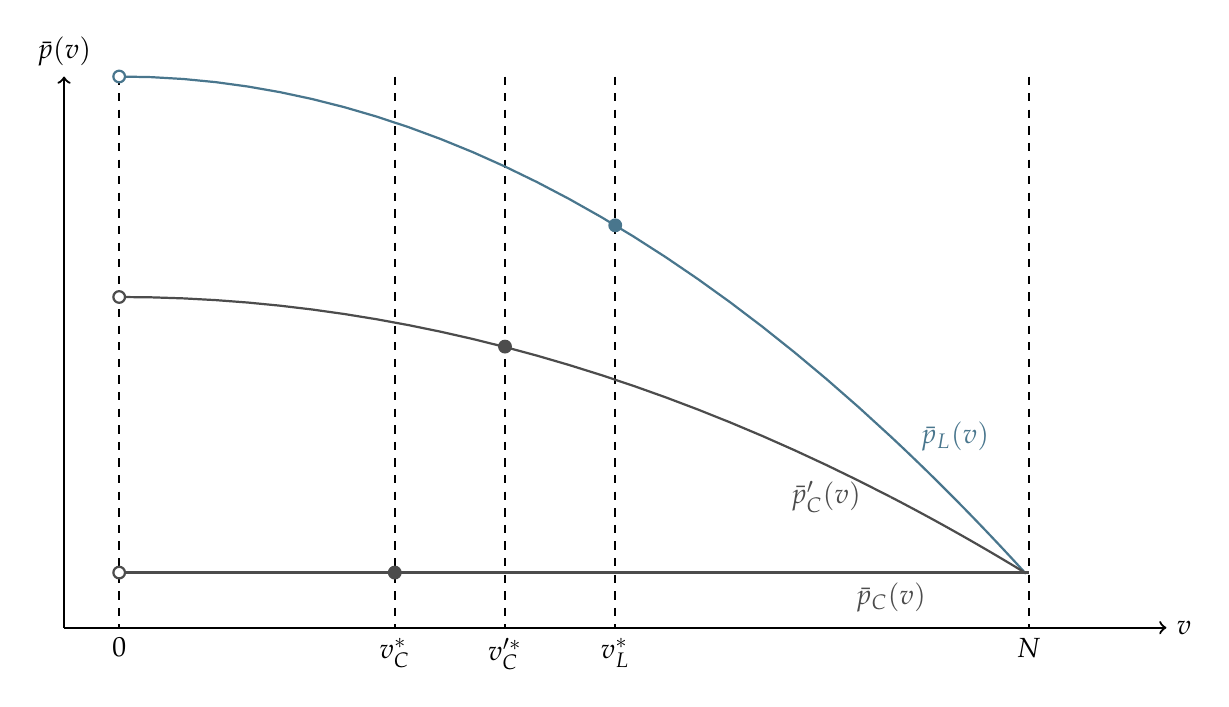
\begin{tikzpicture}[domain=0:100,range=0:200,scale=0.7,thick]
\usetikzlibrary{calc}

% Define linear parameters for supply and demand
\def\inc{10} %Enter total income
\def\pa{1} %Price of x1
\def\pb{1} %Price of x2
\def\panew {0.5} %New price for x1.

% Define coordinates
\coordinate (x2) at (10,10);
\coordinate (x1) at (10,0);
\coordinate (x3) at (0,5);
\coordinate (x4) at (20,5);
\coordinate (x5) at (17.5,10);
\coordinate (x6) at (17.5,0);
\coordinate (x7) at (1,10);
\coordinate (x8) at (1,0);
\coordinate (x9) at (8,10);
\coordinate (x10) at (8,0);
\coordinate (x11) at (6,10);
\coordinate (x12) at (6,0);
\coordinate (p1) at (1,1);
\coordinate (p2) at (1,6);
\coordinate (p3) at (1,10);
\coordinate (p4) at (10,10);

% Draw axes, and dotted equilibrium line
\draw[->] (0,0) -- (20,0) node[right] {$v$};
\draw[->] (0,0) -- (0,10) node[above] {$\bar{p}(v)$};
\draw[thick, dashed] (x2) -- (x1) node[below] {$v^*_L$};
\draw[thick, dashed] (x9) -- (x10) node[below] {$v'^*_C$};
\draw[thick, dashed] (x11) -- (x12) node[below] {$v^*_C$};
\draw[thick, dashed] (x5) -- (x6) node[below] {$N$};
\draw[thick, dashed] (x7) -- (x8) node[below] {$0$};

% Draw indifference curves
\draw[thick,color=cyan!50!black,domain=1:15] plot (\x,{(-(\x-1)^2)/30+10}) node[right] {$\hspace{1.5ex}\bar{p}_L(v)$};
\draw[thick,color=gray!60!black,domain=1:15] plot(\x,{1}) node[below] {$\bar{p}_C(v)$};
\draw[thick,color=gray!60!black,domain=1:15] plot (\x,{(-(\x-1)^2)/54+6}) node[left] {$\bar{p}_C'(v)\hspace{1.5ex}$};
\draw[thick,color=cyan!50!black,domain=15:17.45] plot (\x,{(-(\x-1)^2)/30+10});
\draw[thick,color=gray!60!black,domain=15:17.5] plot(\x,{1}) ;
\draw[thick,color=gray!60!black,domain=15:17.45] plot (\x,{(-(\x-1)^2)/54+6});


% Create points where IC tangentially intersects the budget constraint
\filldraw[color=gray!60!black,fill=white] (p1) circle (3 pt);
\filldraw[color=gray!60!black,fill=white] (p2) circle (3 pt);
\filldraw[color=cyan!50!black,fill=white] (p3) circle (3 pt);

\filldraw[color=gray!60!black,fill=gray!60!black] (6,1) circle (3 pt);
\filldraw[color=gray!60!black,fill=gray!60!black] (8,5.1) circle (3 pt);
\filldraw[color=cyan!50!black,fill=cyan!50!black] (10,7.3) circle (3 pt);
\end{tikzpicture}}
\usebox{\tablebox}\\[1ex]
\parbox{6in}{\footnotesize \textit{Notes:} Curves $\bar{p}_L(v)$, $\bar{p}_C(v)$, and $\bar{p}_C'(v)$ are the average probability of payment among visited property owners by collector type and informedness.  $v^*_k$ are the optimal number of visits selected by collectors, $N$ is the total number of property owners.  This figure displays the case where $E[\lambda_L]=E[\lambda_C]$ and $\rho_L=\rho_C$: the only difference across collector types in average payment probability derives from the level of information about $\lambda_i$'s of property owners and number of properties visited. We discuss this figure in Section \ref{info_adv} and \ref{model_setup}.}
\end{figure}

\clearpage
 
\subsection{Combined Team --- Central X Local}\label{cxl_discussion}

Might combined teams --- pairing chiefs and state agents together --- have promise for raising revenues? This question touches on issues of team production and peer effects, which are beyond the scope of this paper. In our reading, the theoretical literature offers no clear prediction. On the one hand, free-riding issues could be severe \citep{alchian1972}; on the other hand, peer effects and productivity spillovers could outweigh free-riding \citep{kandel1992}. However, \cite{bandiera2010} show that heterogeneity in social ties moderate peer effects, and chiefs and provincial collectors clearly had quite disparate social networks (and other characteristics). We therefore approach this question in a reduced-form way to shed light on whether pairing one chief and one ministry agent together could provide a policy-relevant package. Reasoning that the chief would contribute local information to the team, while the ministry agent would contribute a more credible threat of enforcement, we had expected that ``Central X Local'' (CXL) would outperform Central and Local.\footnote{CXL is also likely easier to implement than CLI, for instance, which reinforces our interest in this arm from a policy perspective.}

However, CXL neighborhoods had tax compliance in between that of Central and Local --- and overall quite similar to CLI. Figure \ref{all_tmts_overtime_bubbles_withCXL} documents a compliance trend over time that approximates a linear combination of that for Central and Local. Table \ref{Table_CvCXL} summarizes these results. On average, CXL had higher compliance than Central, though the effect on revenues is less robust. Local still outperforms CXL.\footnote{As noted when discussing CLI and Local, the change in coefficients for CXL in Columns 1 and 6 derives from the change in the definition of the time period fixed effects described in Section \ref{estimation}, which are defined based on the start and end date of the treatments being compared. Thus, when Local is included in the comparison, the time period definition changes to account for trends in compliance over the full period under examination.} 

We observe no complementarities or positive peer effects between the chief and state collector. As to why the expected complementarities did not materialize, anecdotally, both types of collectors reported coordination issues in this treatment arm. For instance, chiefs and state agents complained of having problems meeting one another at the time specified, and disagreements over who should be in charge of the receipt printer and tax funds. These coordination problems are reminiscent of the challenges encountered in the hybrid subsidy targeting strategy examined in \cite{alatas2012targeting}. However, the trends in compliance (Figure \ref{all_tmts_overtime_bubbles_withCXL})  provide suggestive evidence that the collectors in CXL were perhaps learning how to solve these coordination problems as the campaign went on: they in fact appear better able to counter the secular decline in compliance registered across all other arms. Toward the last period, CXL nearly rivaled Local in compliance. 

In sum, on average, the CXL treatment arm achieved lower revenues than Local, yet it had higher costs (because of greater transport costs for state agents). In this setting, delegating tax collection to chiefs appears preferable on most measurable dimensions compared to a hybrid collection model involving collectors of each type.


\begin{figure}[H]
\textbf{\caption{Decreasing compliance over time --- Central, Local, CXL \label{all_tmts_overtime_bubbles_withCXL}}}
\centering
\scalebox{0.95}{
\includegraphics[scale=0.75]{\folder"/PaperFigure_Compliance_SmoothPlusBubbles_CvLvCXL_2moFE".pdf}
}
\caption*{\footnotesize{\upshape{\textnormal{\textit{Notes}: This figure shows the decrease in compliance for Central, Local, and CLI over the tax campaign. Blue squares represent Local observations, gray circles represent Central observations, and orange diamonds represent CXL observations, with size indicating number of observations.  Lines --- dashed blue for Local, dotted gray for Central, and dashed orange for CXL --- are local linear polynomials estimated separately by treatment.}}}}
\end{figure}

\begin{table}[H]
%\vspace*{-1cm}
\textbf{\caption{\label{Table_CvCXL} Central v. Central X Local}}
\centering
\begin{lrbox}{\tablebox}

\resizebox{15cm}{!}{
\input{output/"Table_CvCXL_MainEffects_HouseFE_edit"}
% OLD: \input{output/"Table_CvCLI_Final_edited"}
}
\end{lrbox}
\usebox{\tablebox}\\[1ex]
\parbox{6in}{\footnotesize \textit{Notes}: This table compares the Central X Local (CXL) arm to the Central arm, which is the excluded category. Columns 1, 5, and 6 report impacts on compliance. Column 2 reports impacts on revenues. Columns 3 and 4 report differences in tax visits by collectors after registration by the extensive and intensive margins, respectively. All regressions include fixed effects for house type, randomization strata, and time periods and cluster standard errors at the neighborhood level. All specifications include time fixed effects defined to maximize overlap between the treatments under comparison, as discussed in Section \ref{estimation}. Column 5 restricts to the subsample of properties that received any tax visits after registration. Column 6 includes a dummy for the Local treatment in the regression. The bottom row reports the $p$-value from a test for equality between the CXL and Local. We discuss these results in Section \ref{cxl_discussion}.}
\end{table}

\subsection{State Collector Team Composition and Performance}
\label{team_composition}

One alternative explanation for the higher compliance achieved in Local is that chiefs worked with assistance and thus benefitted from a naturally hierarchical relationship. In Central, collectors were matched with peers without clear hierarchy. If hierarchy led to more efficient team production \citep{alchian1972}, this team composition difference could account for the gap in tax outcomes between Local and Central. 

To investigate this hypothesis, we exploit the two-staged random assignment of collectors (\textit{i}) into teams, and (\textit{ii}) to neighborhoods to examine if matches of collectors with dissimilar traits corresponds with higher levels of tax compliance and revenue. Specifically, we define a variable \textit{Similarity} that is a dummy for the two randomly assigned collectors both lying either above or below the median for a given collector trait, such as age, education, or income. For instance, in Column 1 of Table \ref{c_cli_team_composition}, \textit{Similarity} equals 1 for all neighborhoods in which both assigned collectors are below the median age as well as for all neighborhoods in which both assigned collectors are above the median age. A negative coefficient would indicate that teams in which the two collectors fall on either side of the median collect more tax, conditional on the average age of the assigned collectors. In fact, we observe that if anything more homogeneous teams of collectors seem to collect more tax. Specifically, collector teams with members who fall on the same side of the median age achieve about 2.9 percentage points higher property tax compliance and 41 Congolese Francs more revenue per owner compared to collector teams that straddle the median age. 

Of course, some teams could straddle the median age but still be only a few years apart. Thus, we also consider the absolute value of the difference between the traits of the two collectors --- in years for age and level of education (Columns 1--2, 4--5, 7--8, and 10--11) and in dollars for income (Columns 3, 6, 9, and 12). We do not observe that a larger difference between the two collectors' traits is correlated with higher performance as a tax collector team. 

\begin{table}[H]
\vspace{.5cm}
\textbf{\caption{State Collector Performance by Team Composition \label{c_cli_team_composition}}}
\centering
\centerfloat
\scalebox{.6}{
\input{\folder"/RV_CvL_Teamwork_TeamComp_edit.tex"}
}
\usebox{\tablebox}\\[1ex]
\parbox{6in}{\footnotesize \textit{Notes}: This table examines the relationship between state collector team structure and tax compliance (Columns 1--6) or tax revenue (Columns 7--12) at the neighborhood level. The variable \textit{Similarity} is a dummy for the two randomly assigned collectors both lying either above or below the median in the collector trait noted in the column titles. \textit{Distance} is the absolute value of the difference between both collectors' traits, measured in years for age and level of education (Columns 1--2, 4--5, 7--8, and 10--11) and in dollars for income (Columns 3, 6, 9, and 12). All regressions include stratum fixed effects, and robust standard errors. In addition, we  control for the average level of the corresponding trait for the assigned collectors in each neighborhood. The sample includes all neighborhoods assigned to Central and CLI, i.e., where state collectors were randomly assigned.}
\end{table}


Thus, at least according to this evidence, we find evidence that heterogeneity in collector teams is not associated with higher performance. There is even some suggestive evidence that homogeneity may lead to higher ability among tax collector teams. In a companion paper \citep{bergeron2019e}, we show that positive assortative matching among tax collectors in the Central arm would increase revenue relative to randomly assigning collectors to each other, which is perhaps consistent with the evidence in Table \ref{c_cli_team_composition}. 

\FloatBarrier
\subsection{Collector Exhaustion and Demoralization}
\label{demoralization}
Another possible mechanism behind the results is that Central collectors become exhausted or demoralized collecting month after month, while chiefs do not because they typically only collect once. Of course, one would anticipate that Central collectors would also have opportunities to learn and improve as collectors over time. Thus, the prediction is theoretically ambiguous. But it is possible that an exhaustion or demoralization effect overpowers learning and this could explain the lower performance of state collectors compared to chiefs.

To investigate this hypothesis, we examine first if state collectors did fewer tax visits over time, and if so whether this decrease is more pronounced compared to the trend in visits in Local. We find evidence that while Central collectors start doing more visits than chiefs, they end doing fewer visits, and the differential trend is statistically significant (Table \ref{TimeInteraction}). 

\begin{table}[ht]
\textbf{\caption{Local v. Central: Visits over Time \label{TimeInteraction}}}
\centering
\scalebox{1}{
\input{\folder"/RV_CvL_Visits_TimeInteraction.tex"}
}
\parbox{\textwidth}{\footnotesize{\textit{Notes}: This table examines visits from tax collector on the extensive (Column 1) and intensive (Column 2) margin across treatments and over time. Specifically, we take deciles of the time distribution of the tax campaign, and interact these with the Local treatment dummy. All regressions include stratum and house type fixed effects, and cluster standard errors at the neighborhood level.}}
\end{table}

Does this decrease in visits over time explain the higher compliance observed in Local neighborhoods? We conduct several analyses to investigate this possibility, and ultimately we find limited evidence to suggest that this mechanism explains the compliance results. 

One test of this mechanism is whether controlling for visits reduces the magnitude of the treatment effect. If the decline in visits were mechanically suppressing tax payment, then controlling for this variable should fully account for the gap in tax compliance we observe between Central and Local. However, when we control for visits on the extensive and intensive margin, the treatment effect on tax compliance stays intact. This analysis involves conditioning on an outcome of treatment, and should thus be interpreted cautiously. We therefore consider several additional tests.

First, we examine compliance comparing Central to the subset of chiefs who collected in multiple neighborhoods. If there is a kind of exhaustion effect that kicks in when collectors work in more than one neighborhood, then these chiefs would have also been affected by this exhaustion effect. However, the gap in compliance between Central and Local restricted to these repeat neighborhood chiefs remains large and statistically significant (Table \ref{compliance_demoral_altsamp}, Column 1). Thus, it does not appear that chiefs collecting in multiple neighborhoods were less effective tax collectors, as might be predicted by a mechanism in which collecting in multiple neighborhoods leads to demoralization and exhaustion with the task. 

Second, we compare Central to a different subset of chiefs who collected in multiple waves of the campaign --- and we restrict Local to chiefs collecting for the second time. If the demoralization effect stems from working on the campaign in two consecutive months, rather than two separate neighborhoods, then one would not predict a difference between Central and ``Repeat Collector Chiefs.'' However, the gap in compliance between Central and Local remains substantial even when restricting to this set of chiefs who had already collected in at least one previous wave (Table \ref{compliance_demoral_altsamp}, Column 3). This analysis should be taken with a grain of salt due to the smaller sample size. However, those chiefs who did work month after month, like the Central collectors, still appear to have collected more tax than state agents.

\begin{table}[ht]
\vspace{.5cm}
\textbf{\caption{Investigating Collector Demoralization and Exhaustion \label{compliance_demoral_altsamp}}}
\centering
\scalebox{1}{
\input{\folder"/RV_CvL_Compliance_DemoralizationChecks_edit.tex"}
}
\parbox{\textwidth}{\footnotesize{\textit{Notes}: This table reports estimates from Equation 1, comparing property tax compliance in Local and CLI to Central (the excluded category). All regressions include fixed effects for randomization strata, house type, and time period fixed effects and cluster standard errors at the neighborhood level. Columns 1--2 restrict the Local sample to neighborhoods where chiefs in charge of collection worked in multiple neighborhoods. Columns 3--4 restrict the Local sample to neighborhoods with chiefs who worked in multiple months (in different neighborhoods), keeping only neighborhoods in their second collection period. Columns 5--6 restrict the Central sample to neighborhoods with state agents collecting for the first time.  The data include all properties registered by tax collectors merged with the government's property tax database.}}
\end{table}

Third, we subset Central to the collectors who were working for the first time. Most of these collectors were from the first wave. But there were 14 other new collectors who joined later in the campaign, too. Thus, ``First Time Central Collectors'' includes neighborhoods in which at least one assigned collector is working on the campaign for the first time. If demoralization kicks in after the first month --- either because of natural exhaustion with the work, or because the comparison with the chiefs becomes more salient --- then comparing this subset of Central collectors to chiefs should reveal no gap between collector types. However, the difference in compliance between treatment arms remains large and statistically significant (Table \ref{compliance_demoral_altsamp}, Column 5). This may be the strongest evidence that a demoralization effect does not appear to explain the gap in compliance and revenue that we observe between chief and state collectors.

Fourth, we use the fact that the same Central collectors at times worked alone and at times consulted with chiefs in CLI. Although the program was designed to minimize contact between chiefs and state collectors --- who were due to visit the tax ministry at different times of the day and of the week, for instance --- the experience of working in CLI might have made salient the fact that chiefs were also working on the tax campaign. If state collectors thought of chiefs as better collectors, this comparison might lead to demoralization after CLI. To test this possibility, we can compare the compliance of Central collectors in the month before CLI and in the month after CLI too see if there is something akin to a trend break --- as would be consistent with the new salience of chief collectors reducing effort or causing demoralization more generally. 

This analysis is made more complicated by the secular decline in compliance across all treatments. To deal with this, we first estimate the trend in compliance in Local neighborhoods only. Then we compare Central neighborhoods before and after CLI, controlling for the trend (in compliance or revenues) estimated in Local.\footnote{More formally, we estimate a parametric event study model around CLI exposure timing that allows for a linear Local trend in time, yielding the impact of exposure to CLI relative to the Local trend \citep{dobkin2018etal, shapiro2019etal}.} We summarize the results in Table \ref{CLIexposure}. While the trend is statistically significant (as expected), we do not observe a systematic additional drop in compliance or revenues in months after Central collectors were exposed to the CLI arm (and thus to chiefs working on the tax campaign). Columns 1 and 3 focus on only the first exposure to chiefs in CLI, which occurred in month 2; these regressions thus compare only compliance and revenue in months 1 and 3. Columns 2 and 4 then also consider if there is an additional drop between month 3 and 5, when Central collectors were again exposed to chiefs in CLI (in month 4). Ultimately, this analysis provides little evidence in support of a demoralization effect driving lower compliance after state collectors have exposure to chiefs in CLI.

\begin{table}[ht]
\textbf{\caption{Central: Exposure to Central + Local Information \label{CLIexposure}}}
\centering
\scalebox{1}{
\input{\folder"/RV_CvL_CLIExposure_edit"}
}
\parbox{\textwidth}{\footnotesize{\textit{Notes}: This table reports changes in compliance and revenues within the Central treatment arm, comparing outcomes before Central agents engaged in consultation with chiefs in the CLI arm with those after consultations took place, for the same set of Central agents. We examine two periods: changes in outcomes between months 1 and 3 (for collectors working in the CLI arm in month 2), and between months 3 and 5 (for collectors working in the CLI arm in month 4).  We exclude the period straddling the final month of CLI (months 5 and 7), as there are few neighborhoods assigned to the Local treatment arm in month 7.  In each period, we estimate the compliance trend in the Local treatment arm and control for it when comparing the pre- and post-periods in the Central treatment arm.  All regressions include house type fixed effects.  When considering multiple periods we include period fixed effects corresponding to the above-described periods.  We do not include fixed effects for stratum or collectors as collectors rotate (due to random assignment to neighborhoods) to different strata and collection partners and thus including these fixed effects would result in a severely restricted sample.}}
\end{table}

Finally, perhaps the most direct test of a pure demoralization explanation is to examine collectors' motivation in the survey we conducted with all collectors --- state and chief --- after the campaign had concluded. In this survey, drawing on the psychology literature \citep{tremblay2009} on motivation, we asked about the extent to which collectors were motivated during the campaign by (\textit{i}) extrinsic motivation (working because of the compensation), (\textit{ii}) intrinsic motivation (working because they found the work intrinsically rewarding), or (\textit{iii}) introjection (working because the job gave them a positive self-image), or (\textit{iv}) goal orientation (working because they thought the work was socially important / their duty). We also asked a module of questions concerning ``amotivation'' that address  demoralization concerns \citep{tremblay2009}. 

We use these questions to compute standardized indices for each motivation type and then compare the levels among chiefs and central collectors at endline. There are no statistically significant differences between collectors concerning the four aforementioned types of motivation (Table \ref{endline_collector_traits}, Rows 1--4). However, we see that chiefs report considerably higher (by 0.42 SDs) levels of amotivation at endline (Row 5). This higher level of demoralization among chiefs is also consistent with the negative point estimates for extrinsic, intrinsic, and goal-oriented motivation (though none of these are statistically significant). Exploring the sub-components of the amotivation index, the coefficient is positive for all three survey questions --- indicating that chiefs were more likely to agree with each of the statements. But the strongest association is a statement asserting that ``our bosses expected too much of us.'' While these results must be taken with a grain of salt because they are self-reported, nonetheless they provide further evidence that the state collectors do not appear to have been more demoralized than the chiefs --- and if anything the opposite may have been true.

\begin{table}[ht]
\textbf{\caption{Local v. Central: Endline Differences in Collector Characteristics \label{endline_collector_traits}}}
\centering
\scalebox{1}{
\input{\folder"/endline_collector_traits_small_edited"}
}
\parbox{\textwidth}{\footnotesize{\textit{Notes}: This table examines endline differences in collector motivation and personality traits using data from a survey conducted with all collectors after the tax campaign. Each row summarizes a regression of the variable noted on an indicator for chiefs who worked in Local (with the omitted category of state collectors who worked in Central). All dependent variables are standardized to facilitate interpretation of magnitudes. The motivation indices in Panel A come from the psychology literature \citep{tremblay2009}. The Big 5 indices come from \cite{borghans2008}. Locus of control questions come from the World Values Survey. The persistence measure is the total number of minutes the collector worked on an impossible maze. The dishonesty/cheating measure involves allocating money between oneself and a payoff to the government according to die rolls, as explained in detail in \cite{lowes2017}.}}
\end{table}


\begin{table}[ht]
\vspace{.5cm}
\textbf{\caption{Local v. Central: Endline Amotivation \label{amotivation}}}
\centering
\scalebox{01}{
\input{\folder"/collector_amotivation_updated"}
}
\parbox{\textwidth}{\footnotesize{\textit{Notes}: This table examines endline differences in collector amotivation using data from a survey conducted with all collectors after the tax campaign. The survey questions were drawn from \cite{tremblay2009}.}}
\vspace{.5cm}
\end{table}

Ultimately, we thus find little evidence to suggest that state collector demoralization or exhaustion led to lower compliance in Central compared to Local. However, it could explain the fact that the slope of the decline in compliance is somewhat more pronounced in Central compared to Local (Figure \ref{all_tmts_overtime_bubbles}).
 
Rather than becoming demotivated, it is also possible that state collectors increased the efficiency of their tax visits thanks to learning by doing --- e.g., by becoming better at targeting high-propensity households. This explanation would be consistent with the evidence in the paper that targeting of visits to households with higher payment propensities is an important mechanism explaining the higher compliance achieved by chiefs in this context. Similarly, the fact that CLI collectors did similar (or smaller) numbers of visits than Central collectors, and yet they collected more revenue, is further evidence that the composition of visits, rather than the number of total visits, is the key driver of collector efficacy in this setting.

Further evidence that Central collectors learned and became more ``efficient'' over time comes from a companion paper in which we examine collector peer effects in the Central arm \citep{bergeron2019e}. In this paper, we show that being matched with a high-type collector --- defined as a collector who achieves a high level of tax compliance across their set of randomly assigned neighborhoods --- in time $t$ causes their partner collector to have higher tax compliance in time $t+1$. Specifically, a 1 SD increase in cumulative exposure to high-type collectors increases tax compliance in subsequent periods by 5.1 percentage points ($p$ = 0.02). However, the partner collector does not exhibit higher effort in $t+1$ in the form of more tax visits. Rather, they seem to get more efficient at collecting taxes conditional on doing a given number of visits. 

\FloatBarrier
\subsection{Quantifying the Knowledge Gap between Chiefs and State Agents}

\label{knowledge_quiz}
The targeting mechanism assumes that chiefs have access to local information that enables them to better target their tax visits to households with higher payment propensities. To illustrate the knowledge levels of both types of collectors, we administered a quiz-type survey module after the tax campaign concluded. Both types of collectors were shown photos of a set of randomly selected property owners in the chief's neighborhood and asked to provide their (\textit{i}) names, (\textit{ii}) jobs, and (\textit{iii}) education levels. We know the correct answers to these questions from household surveys and can therefore estimate a knowledge index for each collector-neighborhood dyad.

Chiefs took the ``quiz'' for their neighborhood, while state collectors took it for neighborhoods where they had not worked to estimate the knowledge they would have had at the outset of the campaign. On average, 2.5 state collectors took the knowledge test for each neighborhood, for whom we compute the average accuracy and compare this to the local chief's score. In comparing collector types, we exclude chiefs in Local and CXL because they may have learned about their neighborhoods from collecting taxes. Thus, we restrict the sample of chiefs to all neighborhoods where chiefs did not work as tax collectors (i.e., Central, CLI, and pure control). According to this analysis, chiefs were indeed much better informed about the residents of their neighborhoods than state collectors, scoring about 70\% more accurately on this quiz (Figure \ref{C_L_knowledge}). 

\begin{figure}[H]
\textbf{\caption{Knowledge Quiz: State Collectors v. Non-Collector Chiefs  \label{C_L_knowledge}}}
\centering
%\centerfloat
\begin{tabular}{cc}
\\
\includegraphics[scale=1]{{\folder"/KnowsIndex_C_vs_L_NonCollectorChiefs"}.pdf} \\
\end{tabular}
\parbox{\textwidth}{\footnotesize{\upshape{\textnormal{\textit{Notes}: This figure shows the distributions of knowledge about citizens for chiefs compared to state collectors. Knowledge of the inhabitants of the neighborhood is measured by the percentage of correct answers regarding a random sample of property owners in a short quiz-type survey module conducted after tax collection. Questions included the owner's name, education level, and occupation. Chiefs took quizzes for their own neighborhoods, but we restrict the sample to chiefs who did not collect taxes (since the quiz was administered after the campaign); central agents took quizzes for randomly selected neighborhoods to simulate the knowledge they would have if assigned to a location before collecting taxes there. We discuss these results in Section \ref{info_adv}.}}}}
\end{figure}

\subsection{The Limits to Codifying Local Information} 
\label{codifiability}

Information is a pillar of state capacity. States must render society ``legible'' in order to raise revenue and pursue other state-building projects \citep{scott1998seeing}. The paper provides direct evidence of the value of local information possessed by city chiefs in raising tax compliance. When equipped with local information, state collectors raised 30.9\% more revenue. 

However, the results also highlight the limits of the state's ability to codify and harness local information. Some information possessed by chiefs and useful for tax collection appears to have been simply uncodifiable. This conclusion stems from the combination of two observations: (\textit{i}) Local realized higher tax compliance than CLI, and (\textit{ii}) chiefs did not exhibit greater persuasive power. The remaining gap likely reflects the uncodifiable information of the chief that is relevant for tax collection, including ``tacit knowledge'' about payment propensities of households \citep{polanyi1958}.\footnote{\cite{polanyi1958} coined the term tacit knowledge for abilities like facial recognition or language learning that cannot be easily expressed as the sum of explicit, codifiable facts. \cite{williamson1979} draws on this idea when discussing the appropriate governance structures in markets high in idiosyncratic transaction-specific human capital. \cite{ober2008} emphasizes the social value of political institutions capable of integrating technical and tacit knowledge.} 

What aspects of local information are uncodifiable? If such information were truly akin to tacit knowledge, then by definition we could not perfectly characterize it. However, we can compare characteristics of households who were visited after registration in Local and CLI and examine where they diverge. Overall, the characteristics of households visited in CLI are closer to those visited in Local than Central, on both visible and non-visible dimensions (Figure \ref{fig:main_targeting1}).\footnote{The similarity between the implied targeting functions of collectors in CLI and Local (rather than Central) provides further evidence about the compositional shift in targeting that led state collectors in CLI to achieve higher compliance than those in Central, as discussed in Section \ref{targeting}.} Comparing CLI to Local, the clearest difference concerns liquidity (Figure \ref{main_targeting_appendix_LvCLI}), with CLI collectors somewhat less likely to have visited above-median liquidity households ($p$ = 0.089). The uncodifiable component of chiefs' information may thus concern household liquidity. For instance, one possibility is that chiefs received signals about the \textit{timing} of households' liquidity constraints that enabled them to better target tax visits on the time dimension of payment propensity as well as on time-invariant dimensions (e.g., households' underlying tax morale). Such knowledge would have been difficult to convey in a one-off consultation with state collectors. We find suggestive evidence of this possibility by analyzing the time stamps on receipt data, which reveal similar distributions of tax collections occurring primarily in the morning with one crucial difference: chiefs also collected collected a small share of taxes in the evening (Figure \ref{time_collection_CvLvCLI}). This difference in evening collection could explain 40.1\% of the remaining revenue gap between Local and CLI. 

%time dimension
An alternative interpretation is that chiefs possessed other (codifiable) information that they simply chose not to share during consultations with state collectors in CLI. Although we cannot rule it out entirely, this interpretation appears unlikely given that the households recommended by chiefs in CLI resemble closely the households that chiefs themselves targeted in Local neighborhoods.\footnote{The co-movement of CLI and Local in terms of tax visits and their correlations with household characteristics is evident in Figure \ref{fig:main_targeting1} as well as Table \ref{validation_cli_control}.} Moreover, anecdotal evidence from state collectors and program supervisors confirms that chiefs were sincerely engaged during CLI consultations.\footnote{For instance, as noted above, chiefs suggested adding ``willingness to pay'' --- in addition to ``ability to pay'' --- as a field on the form state collectors' filled out during the consultations. They felt an important dimension about households' payment propensity was not reflected in the codification of their knowledge, and unprompted they suggested an amendment to the protocol.} All told, the results suggest that, in urban settings of low state capacity, the government can achieve better outcomes --- from the perspective of the state coffers as well as that of citizens --- by delegating collection responsibilities to local elites rather than by trying to integrate their local information into state collection.
%\footnote{This conclusion is consistent with recent work on hybrid institutions in settings of conflict and fragility \citep{boege2009, heald2007}.} - ADD BACK LATER


\begin{figure}[H]
%\vspace*{-1cm}
\centering{}\caption{Timing of Tax Collections by Treatment \label{time_collection_CvLvCLI}}
\includegraphics[scale=0.9]{\folder"/time_collection_CvLvCLI"}
\usebox{\tablebox}\\[1ex]
\parbox{6in}{\footnotesize \textit{Notes}: This figure shows the distribution of tax payments according to the receipt data. We discuss these findings in Section \ref{info_adv}.}
\end{figure}

\subsection{Cost-Effectiveness}
\label{cost_effectiveness}

To estimate the cost-effectiveness of state and chief tax collection, we examine campaign data on the marginal costs of tax administration, including transport costs and collector compensation.\footnote{Transportation costs, in particular, are emphasized in theoretical work on the tradeoffs between centralized collection and taxation by local elites \citep{azabou1988contractual, levi1989rule}.} State collectors were reimbursed for motorcycle taxis from the provincial tax ministry to their assigned neighborhoods. Chief collectors, by contrast, did not incur such costs because they worked near their homes. They were, however, reimbursed for weekly trips to the tax ministry to deposit their tax receipts and receive their bonus. The other key marginal cost was collectors' compensation, which was constant across treatments.

The marginal costs associated with Central and Local are summarized in Figure \ref{fig:costs_all} (Panel A). Chief tax collection has roughly 30\% lower administrative costs than state collection. Panel B shows back-of-the envelope estimates of the treatments' cost-effectiveness. The return on \$1 is 53\% higher in Local compared to Central due to the higher revenues achieved as well as the decreased administrative costs. Moreover, while Local was cost-effective, Central on average was not.\footnote{At the outset of the campaign, state collection was also cost-effective. But the secular decline in tax compliance over 2018 meant that over the course of the campaign, administration costs exceeded tax revenues.} Further, this analysis reveals heterogeneity that could guide future policy. State collectors were similar to chiefs in cost-effectiveness when working in the city center, whereas they were much less cost-effective in the city's peripheries (Figure \ref{cea_remoteness}). Depending on its assessment of the social cost of bribery (cf. Section \ref{bribe_multiplier_discussion}), governments could opt for collection strategies involving state agents in the city center and chiefs in the periphery.

Although the revenue returns to tax administration costs were low, this is a setting of near-zero prior citizen compliance in which the government is making initial investments in fiscal capacity that it hopes will lead to higher revenues over time. Tax officials often discuss their objective of gradually inculcating a ``fiscal culture'' in Kananga. In other words, the government expects positive inter-temporal spillovers that make the expected future return higher than our calculations. In Section \ref{external_validity_model}, we discuss how contextual differences and broader fiscal capacity investments could alter the choice of collector type. Yet even low-cost investments, such as mobile remittance of taxes by collectors (already on the tax ministry's agenda), could have large revenue impacts.\footnote{Mobile banking and money transfer services are already widely used in Kananga.} If chief collectors did not have to make weekly (or biweekly) trips to the government to deposit collections and receive their compensation, we estimate that \$1 spent on chief collection would generate \$2.1, as shown in Panel B of Figure \ref{fig:costs_all}.

\begin{figure}[H]
\centering{}\caption{Costs and cost-effectiveness across treatments \label{fig:costs_all}}
\begin{tabular}{c}
A: Costs of Tax Collection Methods \\
\includegraphics[scale=.8]{output/"costs_by_treatment"} \\
\\
B: Cost-Effectiveness of Tax Collection Methods  \\
\includegraphics[scale=.8]{output/"marginal_revenue_hypothetical"}\\
\end{tabular}
\parbox{6in}{\footnotesize \textit{Notes}: This figure reports estimated costs (Panel A) and cost-effectiveness (Panel B) for the Central and Local treatments. In Panel A, costs are broken down by transport and compensation. In Panel B, cost-effectiveness is the return of an additional \$1 spent on collection in particular treatment, and the hypothetical cost-effectiveness of Local with mobile payments is shown at far right. Estimates are the mean value of each measure averaging across neighborhoods.  Confidence intervals are shown by the vertical bars. We discuss these results in Section \ref{cost_effectiveness}.}
\end{figure}


\begin{figure}[H]
\centering{}\caption{Cost-effectiveness of Local and Central by Remoteness \label{cea_remoteness}}
\includegraphics[scale=.8]{output/"scatter_benefit_cost_dist_center_CvsL"}
\parbox{6in}{\footnotesize \textit{Notes}: This figure reports estimated cost-effectiveness for the Central and Local treatments as a function of the distance from downtown Kananga. We discuss these results in Section \ref{cost_effectiveness}.}
\end{figure}


\begin{table}[H]
%\vspace*{-1cm}
\textbf{\caption{\label{bribe_multiplier} Local v. Central: Bribe Multiplier}}
\centering
\begin{lrbox}{\tablebox}
\resizebox{15cm}{!}{
\input{output/AppdxPaperTable_BribeMultiplier_edit}
}
\end{lrbox}
\usebox{\tablebox}\\[1ex]
\parbox{6in}{\footnotesize \textit{Notes}: This table reports measures from the tax campaign of total revenues collected and costs incurred for the Central and Local treatment arms. Columns 1 and 4 report revenues collected by treatment arm. Columns 2 and 5 report costs, which include bonuses paid to tax collectors and compensation  for transportation.  The second row reports costs under a hypothetical system in which chief collectors were paid (and remit tax collections) via mobile money rather than visiting the tax ministry to receive bonuses (and deposit collections). Costs for Central under this alternative system would remain the same. Columns 3 and 6 show the amounts of bribes collecting according to the measure at endline, scaled by the number of individuals surveyed at endline relative to the neighborhood population of households.  All amounts are in Congolese Francs.  Column 7 reports the implied multiplier on bribe payments that would be required for the government to weakly prefer employing state collectors instead of chief collectors: $\Gamma=((R_L-R_C)-(C_L-C_C))/(B_L-B_C)$. This formula is discussed in more detail in Section \ref{model_setup}. We discuss these results in Section \ref{cost_effectiveness}.}
\end{table}

\clearpage
\pagebreak


\section{Ethical Considerations}

The design of this study involved careful consideration of the potential risks to participants. In the following sections, we provide details on these risks and how we endeavored to minimize them, as well as the ethics review process we undertook.

\medskip

\textbf{IRB Approval.} We obtained approval from Harvard University (protocol IRB17-0724) in 2017, before commencing field research. Our submission outlined the experimental design and included all survey instruments, consent forms, and other material needed to judge the potential risks and benefits to research participants. Although the D.R. Congo does not have a national ethics board, we sought out local ethical approval from the oldest and most highly regarded university in Kananga, the University of Notre-Dame du Kasa\"i. We submitted the same set of materials and our Harvard IRB protocol to the academic dean of the university. We received a formal approval letter in 2017. 

\medskip

\textbf{Compensation.} Randomly sampled participants in the surveys we administe\-red received compensation to thank them for their time. They were informed of the compensation during the consent, and then received the compensation at the end of the survey. Participants received approximately USD\$2 per hour of survey. Thus, the baseline survey took roughly 1 hour, and individuals received USD\$2. The midline survey took 20--30 minutes, and individuals received USD\$1. The endline survey took 90--120 minutes, and individuals received USD\$4. We have used a similar survey respondent compensation amount in Kananga since 2013. We chose this amount based on how other international organizations had comp\-ensated survey respondents in the city in the past. 

\medskip

\textbf{Risks and benefits.} In designing the study, we judged the risks to participants to be minimal, in other words, no greater than those they would encounter in the study's absence. Concerning benefits, the data we collected from human subjects enabled us to write an evaluation that may help the government to reduce the incidence of bribe taking and to increase its revenues. We discuss each of these in turn.

\medskip

The principal risk facing our participants, a random sample of the city populat\-ion of Kananga, concerned potentially sensitive and identifiable data falling into the hands of other actors, such as the government. There were two primary sensitive topics broached in the surveys. 

First, in our surveys, we asked questions about tax payment, bribe payment, as well as attitudes about the government. Since the topics of taxation and corrup\-tion concern behavior deemed illegal by Congolese Law, these data were highly sensi\-tive. We were particularly concerned about the government gaining access to survey data and using these data to pursue sanctions against non-compliant (or bribe-paying) households. This was one important risk faced by survey parti\-cipants. 

Second, we also asked questions about the local city chief: their behavior during the tax campaign, their solicitation of bribes, their enforcement of other informal sanctions in the neighborhood among non-compliant households, as well as respondents' views of and trust in city chiefs. We were similarly concerned that these data could fall into the hands of the neighborhood chief and that there could thus be negative consequences among our survey participants. 

After consulting with the Harvard IRB and the University of Notre-Dame du Kasa\"i academic dean, we undertook a number of steps to mitigate these risks as much as possible. We collected all data on password-protected tablets, and we wiped the memory of these tablets on a regular basis. The survey program we use (ODK) also stores responses in XML format and in a folder on the tablet that is difficult to access and interpret unless an individual has prior training. If a government official or the chief gained access to a tablet, they would have had a difficult time accessing the data. We then stored the identifiable data in our research office on password-protected computers. The office is in a walled compound that is guarded 24-7. 

In light of these measures, we believe that participation in the study would not represent greater risk than respondents might encounter in their daily lives. Fortunately, there were no instances of lost or stolen tablets during the study, nor reports of theft from the research office.

The benefits of participating in this study --- in a research ethics sense distinct from compensation --- would primarily accrue at the societal level. Although we did not share identifiable or disaggregated survey data with the government, we did provide a report of our analysis of the impacts of the tax campaign on tax compliance, revenues, and bribe payment. The survey data was an essential component of this report, and it will help the government to improve its tax collection policies in the future. 

Such improvements could lead to benefits to citizens in both direct and indi\-rect ways. In terms of more direct social benefits, our evaluation should help the government in its efforts to reduce corruption and bribes collected by tax collect\-ors by providing information about the level and nature of bribe-taking. To the extent that our evaluation helps the government learn how to collect more tax, this could enable the government to provide more public goods in Kananga. Indeed, revenues are sorely needed by the provincial government, which coll\-ected on average USD\$0.30 per person in the province in 2015. As we note in the paper, low tax capacity is widely regarded as a key development challenge in low-income countries like the DRC \citep{besley2009origins}. 

Regarding indirect benefits, there is evidence that taxation can help promote a social contract between citizens and the government. Indeed, past evidence from the 2016 tax campaign in Kananga suggested that property tax collection raised citizen engagement with the provincial government \citep{weigel2019}. We therefore view evaluations of policies used by the provincial government to expand its fiscal capacity as helping to usher in a range of governance benefits related to the tax-based social contract.

\medskip

\textbf{Discussion.} In light of the potential risks, our measures to mitigate them, and the potential societal benefits from evaluating government tax policies, we firmly believe that this research meets widely accepted ethical standards for social sci\-ence research. As indicated by the IRB approvals we received from Harvard University and the University of Notre-Dame du Kasa\"i, the risk-benefit ratio was also judged to be favorable by two different independent bodies with expertise in research ethics.

In addition to the specific risks and benefits to survey participants enumerated above, we discuss here several other ways in which we were involved in the taxation campaign and the possibility that by evaluating this tax campaign imple\-mented by the government our mere presence as international researchers could influence its outcomes in more subtle ways. We also noted these points in our IRB submi\-ssions.

First, the government had planned to collect property taxes and to involve the same types of tax collectors regardless of whether we conducted an evaluation of the campaign. However, the assignment of collectors to different neighborhoods would have not likely been randomized absent the involvement of researchers. As noted in the paper, we conducted the randomization that was ultimately used for the implementation of the tax campaign of 2018. Relatedly, we consulted with the government regarding other elements of the policy experiment design, including (\textit{i}) the number of neighborhoods allocated to each treatment arm, (\textit{ii}) the timing of different waves of the campaign across treatments, (\textit{iii}) the randomi\-zation of messages on tax letters, and (\textit{iv}) the mechanics of the Central + Local Information treatment arm. 

To inform the allocation of neighborhoods to treatments, we conducted power calculations using data from the logistical pilot of the different types (and combi\-nations) of tax collectors in early 2018. The final allocation included the largest number of neighborhoods in the Central and Local treatment arms, the primary comparison of the policy experiment. Central + Local Information (CLI) had somewhat fewer neighborhoods as a secondary comparison. During the logistics pilot, the Central X Local (one chief and one state collector) teams achieved the highest compliance, so we anticipated it would require relatively less sample to distinguish compliance in this treatment relative to the other treatments. 

Given that there was considerable uncertainty ex ante about the outcomes of the different tax collection treatments examined in the context of the 2018 campaign, our position is that randomization was the most equitable way to assign tax collection responsibilities, and likewise for the use of randomization in allocating neighborhoods to different waves of the campaign and assigning message treatments on tax letters. We were pleased to assist the government to do this using our technical background in power calculations and randomized controlled trials more generally. 

Regarding the design of the CLI arm, we helped the government during the logistics pilot to evaluate different approaches of transferring knowledge of the neighborhood chief to state collectors. To do this, we interviewed a number of collectors and city chiefs from the pilot neighborhoods. We then synthesized the findings from this process as well as quantitative data from the pilot for the government. As with our role in evaluating the impact of the overall campaign on government revenue, these inputs in the pilot stage of CLI were necessary to learn as much as possible from the campaign about the emergence of tax capacity in weak-state settings.

Second, we conducted technical trainings for tax ministry staff who worked on the tax campaign regarding the receipt printers used by tax collectors. Altho\-ugh these technologies had been purchased by the government in 2015 from an Indian company (KS Infosystems), outside of a handful of tax collectors working at the city's tolls and airport, few tax ministry staff were familiar with the receipt printers and the management of the database associated with them. We therefore helped adapt these devices for collection of the property tax and conducted a series of trainings on the use of these technologies (and the management of data).\footnote{In fact, we suggested the government consider an alternative receipt printing technology, but the tax ministry leadership chose to continue using the KS machines for the 2018 campaign.} None of this involvement relates to experimental variation we study in the rese\-arch. We view these trainings as important investments in the technical capacity of the provincial government. The goal of the government in using the handheld receipt printers was to create a paper trail for tax collectors in order to enhance monitoring capacity and reduce the payment of bribes. We were pleased to help the government with this goal. 

Third, it is possible that the very fact of our conducting an evaluation of this campaign may have changed the behavior of tax collectors or other government officials, akin to a more macro-level ``Hawthorne Effect.'' We of course cannot rule out this possibility because we do not observe the counterfactual campaign (in which we did not conduct an evaluation). However, we suspect any such influences would likely be benign from a research ethics point of view.\footnote{From an internal validity perspective, we took steps to ensure that any information about our evaluation was kept constant across treatment groups. For instance, all tax collector trainings were identical.} For instance, if tax collectors learned of the surveys our enumerators were conducting in the city to evaluate the campaign, it would have most likely led them to behave in a more professional manner and to collect fewer illicit payments. We do not think there are plausible scenarios in which awareness of the evaluation could have created incentives for collectors to act in ways that would reduce the welfare of average citizens in Kananga. This is all of course quite speculative, and we do not wish to overestimate our ability to predict the direction of such big-picture ``Hawthorne Effects.'' However, we wanted to note that these were factors we took into consideration when deciding whether and how to conduct this research.

\medskip


\end{document}
